\documentclass[11pt,a4paper]{article}

% --- Layout: A4 quer + 2 Seiten auf 1 Blatt ---
% --- Layout: 2 Seiten auf 1 Blatt (A4 quer) ---
\usepackage[a4paper,left=10mm,right=10mm,top=10mm,bottom=10mm]{geometry}
\usepackage{pgfpages}
\pgfpagesuselayout{2 on 1}[a4paper,landscape,border shrink=3mm]

% --- Sprache / Text ---
\usepackage[T1]{fontenc}
\usepackage[utf8]{inputenc}
\usepackage[ngerman]{babel}

% --- Mathe / Listen ---
\usepackage{amsmath,amssymb}
\usepackage{enumitem}
\setlist[itemize]{noitemsep,topsep=2pt}
% --- Code Styling ---
\usepackage{xcolor}
\usepackage{listings}

% Farben
\definecolor{codebg}{RGB}{248,248,248}
\definecolor{codeframe}{RGB}{220,220,220}
\definecolor{codekw}{RGB}{0,92,185}
\definecolor{codestr}{RGB}{180,60,20}
\definecolor{codecom}{RGB}{90,110,90}
\definecolor{codeid}{RGB}{70,70,70}
\definecolor{codeemph}{RGB}{155,0,90}

% Inline-Highlight (für wichtige Wörter im Text)
\newcommand{\hilite}[1]{\colorbox{yellow!25}{#1}}
\newcommand{\imp}[1]{\textbf{\textcolor{codeemph}{#1}}}
\newcommand{\kw}[1]{\textbf{\textcolor{codekw}{#1}}}

% Listings: Grundstil
\lstdefinestyle{vhdl}{
  backgroundcolor=\color{codebg},
  frame=single,
  rulecolor=\color{codeframe},
  frameround=tttt,
  basicstyle=\ttfamily\footnotesize,
  keywordstyle=\bfseries\color{codekw},
  commentstyle=\itshape\color{codecom},
  stringstyle=\color{codestr},
  identifierstyle=\color{codeid},
  numbers=left,
  numberstyle=\tiny\color{codeid},
  numbersep=6pt,
  tabsize=2,
  showstringspaces=false,
  breaklines=true,
  upquote=true
}

% VHDL Sprache definieren (listings hat VHDL meist, aber so bist du safe)
\lstdefinelanguage{VHDL}{
  morekeywords={
    library,use,all,entity,is,port,generic,begin,end,architecture,of,signal,
    constant,type,record,array,process,if,then,elsif,else,when,case,others,
    loop,for,to,downto,generate,return,function,procedure,variable,shared,
    rising_edge,assert,report,severity
  },
  sensitive=true,
  morecomment=[l]--,
  morestring=[b]"
}

% Default für deine Codeblöcke
\lstset{style=vhdl,language=VHDL}

% Optional: XDC/Tcl als zweite Sprache (für Constraints)
\lstdefinestyle{xdc}{
  backgroundcolor=\color{codebg},
  frame=single,
  rulecolor=\color{codeframe},
  frameround=tttt,
  basicstyle=\ttfamily\footnotesize,
  keywordstyle=\bfseries\color{codekw},
  commentstyle=\itshape\color{codecom},
  stringstyle=\color{codestr},
  numbers=left,
  numberstyle=\tiny\color{codeid},
  numbersep=6pt,
  tabsize=2,
  showstringspaces=false,
  breaklines=true
}

% --- Grafiken ---
\usepackage{graphicx}
\usepackage{subcaption}

% --- Typografie kompakt ---
\usepackage{microtype}
\usepackage{parskip}
\setlength{\parskip}{2pt}
\setlength{\parindent}{0pt}
\renewcommand{\baselinestretch}{0.95}
\small

\title{Digital Microelectronics}
\author{Näf Gian Marco}
\date{\today}
\usepackage{hyperref}
\begin{document}
\maketitle



% ============================================================
\section{How to Design a System on Chip}

\subsection{Motivation und Einordnung}
Moderne digitale Systeme sind durch steigende Komplexität, hohe Heterogenität und starken Zeitdruck geprägt. Klassische FPGA- oder HDL-basierte Schaltungsentwicklung skaliert nicht mehr. Aktuelle Designs sind vollständige Systeme mit Prozessoren, Speicherhierarchien, Peripherie und applikationsspezifischer Logik auf einem einzigen Chip.

\subsection{Begriff und Eigenschaften eines SoC}
Ein System on Chip integriert Mikroprozessor(en), Speicher, Standardperipherie und anwendungsspezifische IP-Blöcke auf einem Silizium-Die. Ziel ist eine hohe Integrationsdichte bei reduzierten Entwicklungs- und Systemkosten sowie erhöhter Flexibilität durch Software-Updates und rekonfigurierbare Hardware.

FPGA-basierte SoCs kombinieren feste Hard-IP (Processing System) mit rekonfigurierbarer Logik (Programmable Logic). Dies erlaubt Hardware/Software-Co-Design und iterative Systementwicklung.

\subsection{Zynq-7000 Architekturüberblick}
Die Zynq-7000 Plattform besteht aus zwei Hauptdomänen:
\begin{itemize}
  \item \textbf{Processing System (PS):} Dual ARM Cortex-A9, Caches, Speichercontroller, feste Peripherie, Hard-IP.
  \item \textbf{Programmable Logic (PL):} 7-Series FPGA-Logik mit CLBs, Block RAM, DSP48E1-Slices, I/O-Blöcken und Clock-Ressourcen.
\end{itemize}

PS und PL sind eng gekoppelt und kommunizieren über dedizierte AXI-Interfaces. Ergänzt wird das System durch analoge Funktionen wie XADC (ADC, Sensorik).

\begin{figure}[t]
  \centering
  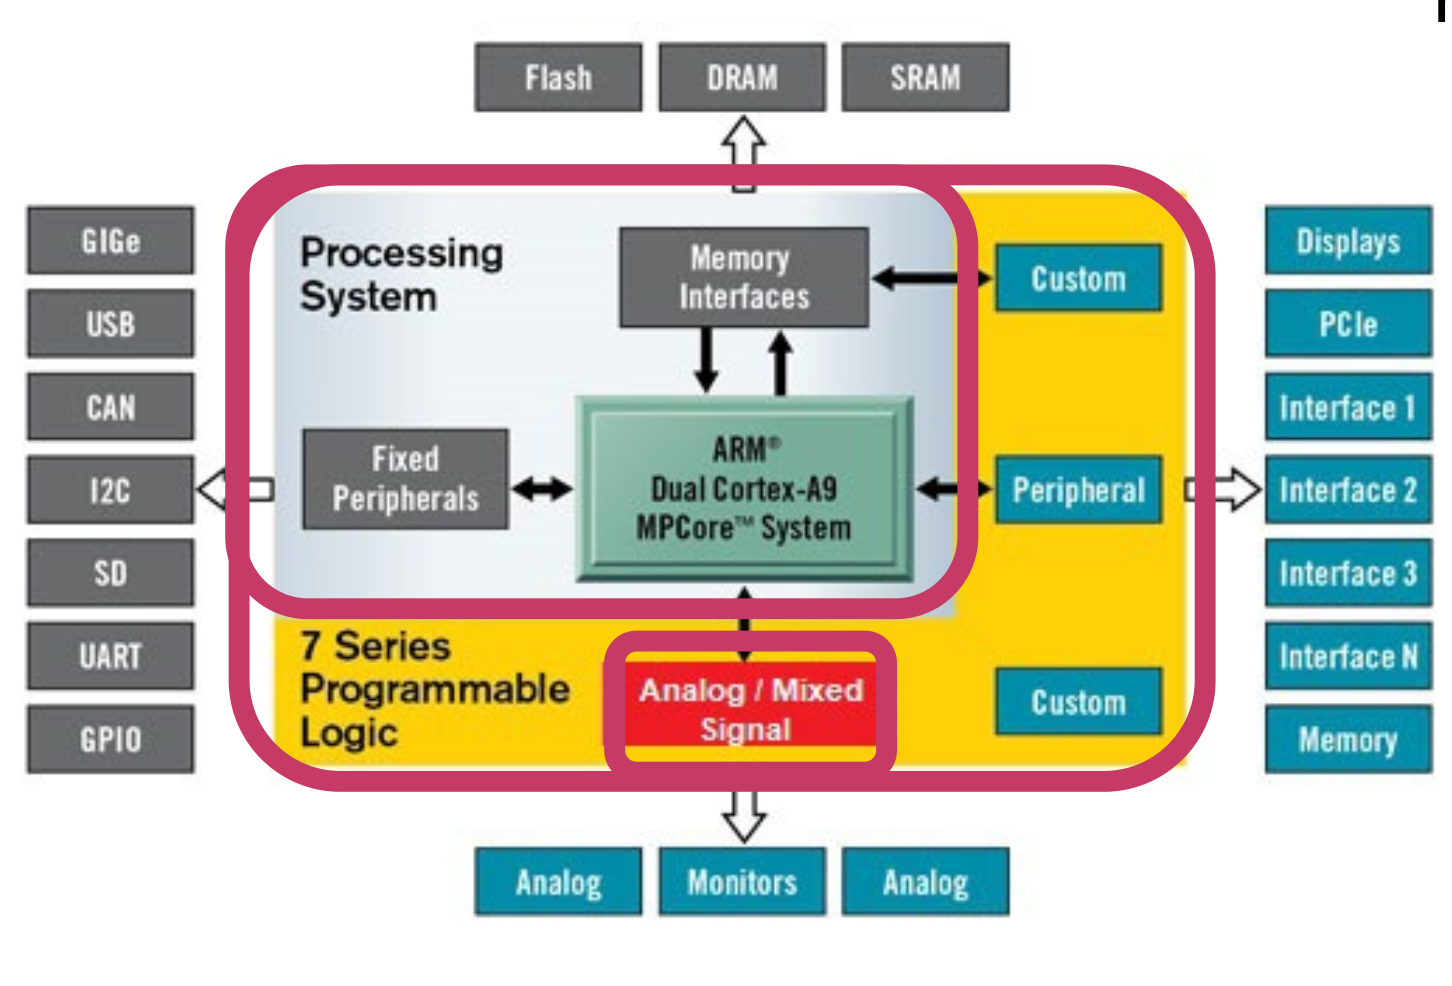
\includegraphics[width=\linewidth,height=0.28\textheight,keepaspectratio]{fig/L1_zynq_arch.png}
  \caption{Zynq-7000 Gesamtarchitektur (PS/PL).}
\end{figure}

\subsection{Ressourcen der Programmable Logic}
Die PL basiert auf einer feingranularen Logikstruktur:
\begin{itemize}
  \item \textbf{CLB (Configurable Logic Block):} Besteht aus zwei Slices.
  \item \textbf{Slice:} Enthält LUTs, Flip-Flops, Carry-Chains und Multiplexer.
  \item \textbf{LUTs:} 6-Eingangs-LUTs mit Dual-Output, konfigurierbar als zwei 5-Eingangs-LUTs.
  \item \textbf{Block RAM:} Dual-Port, vollständig synchron, optional gepipelined.
  \item \textbf{DSP48E1:} Multiplizierer, Pre-Adder, Post-Adder, SIMD-fähig.
\end{itemize}

Diese Ressourcen ermöglichen hochparallele, datenpfadorientierte Implementierungen.

\begin{figure}[t]
  \centering
  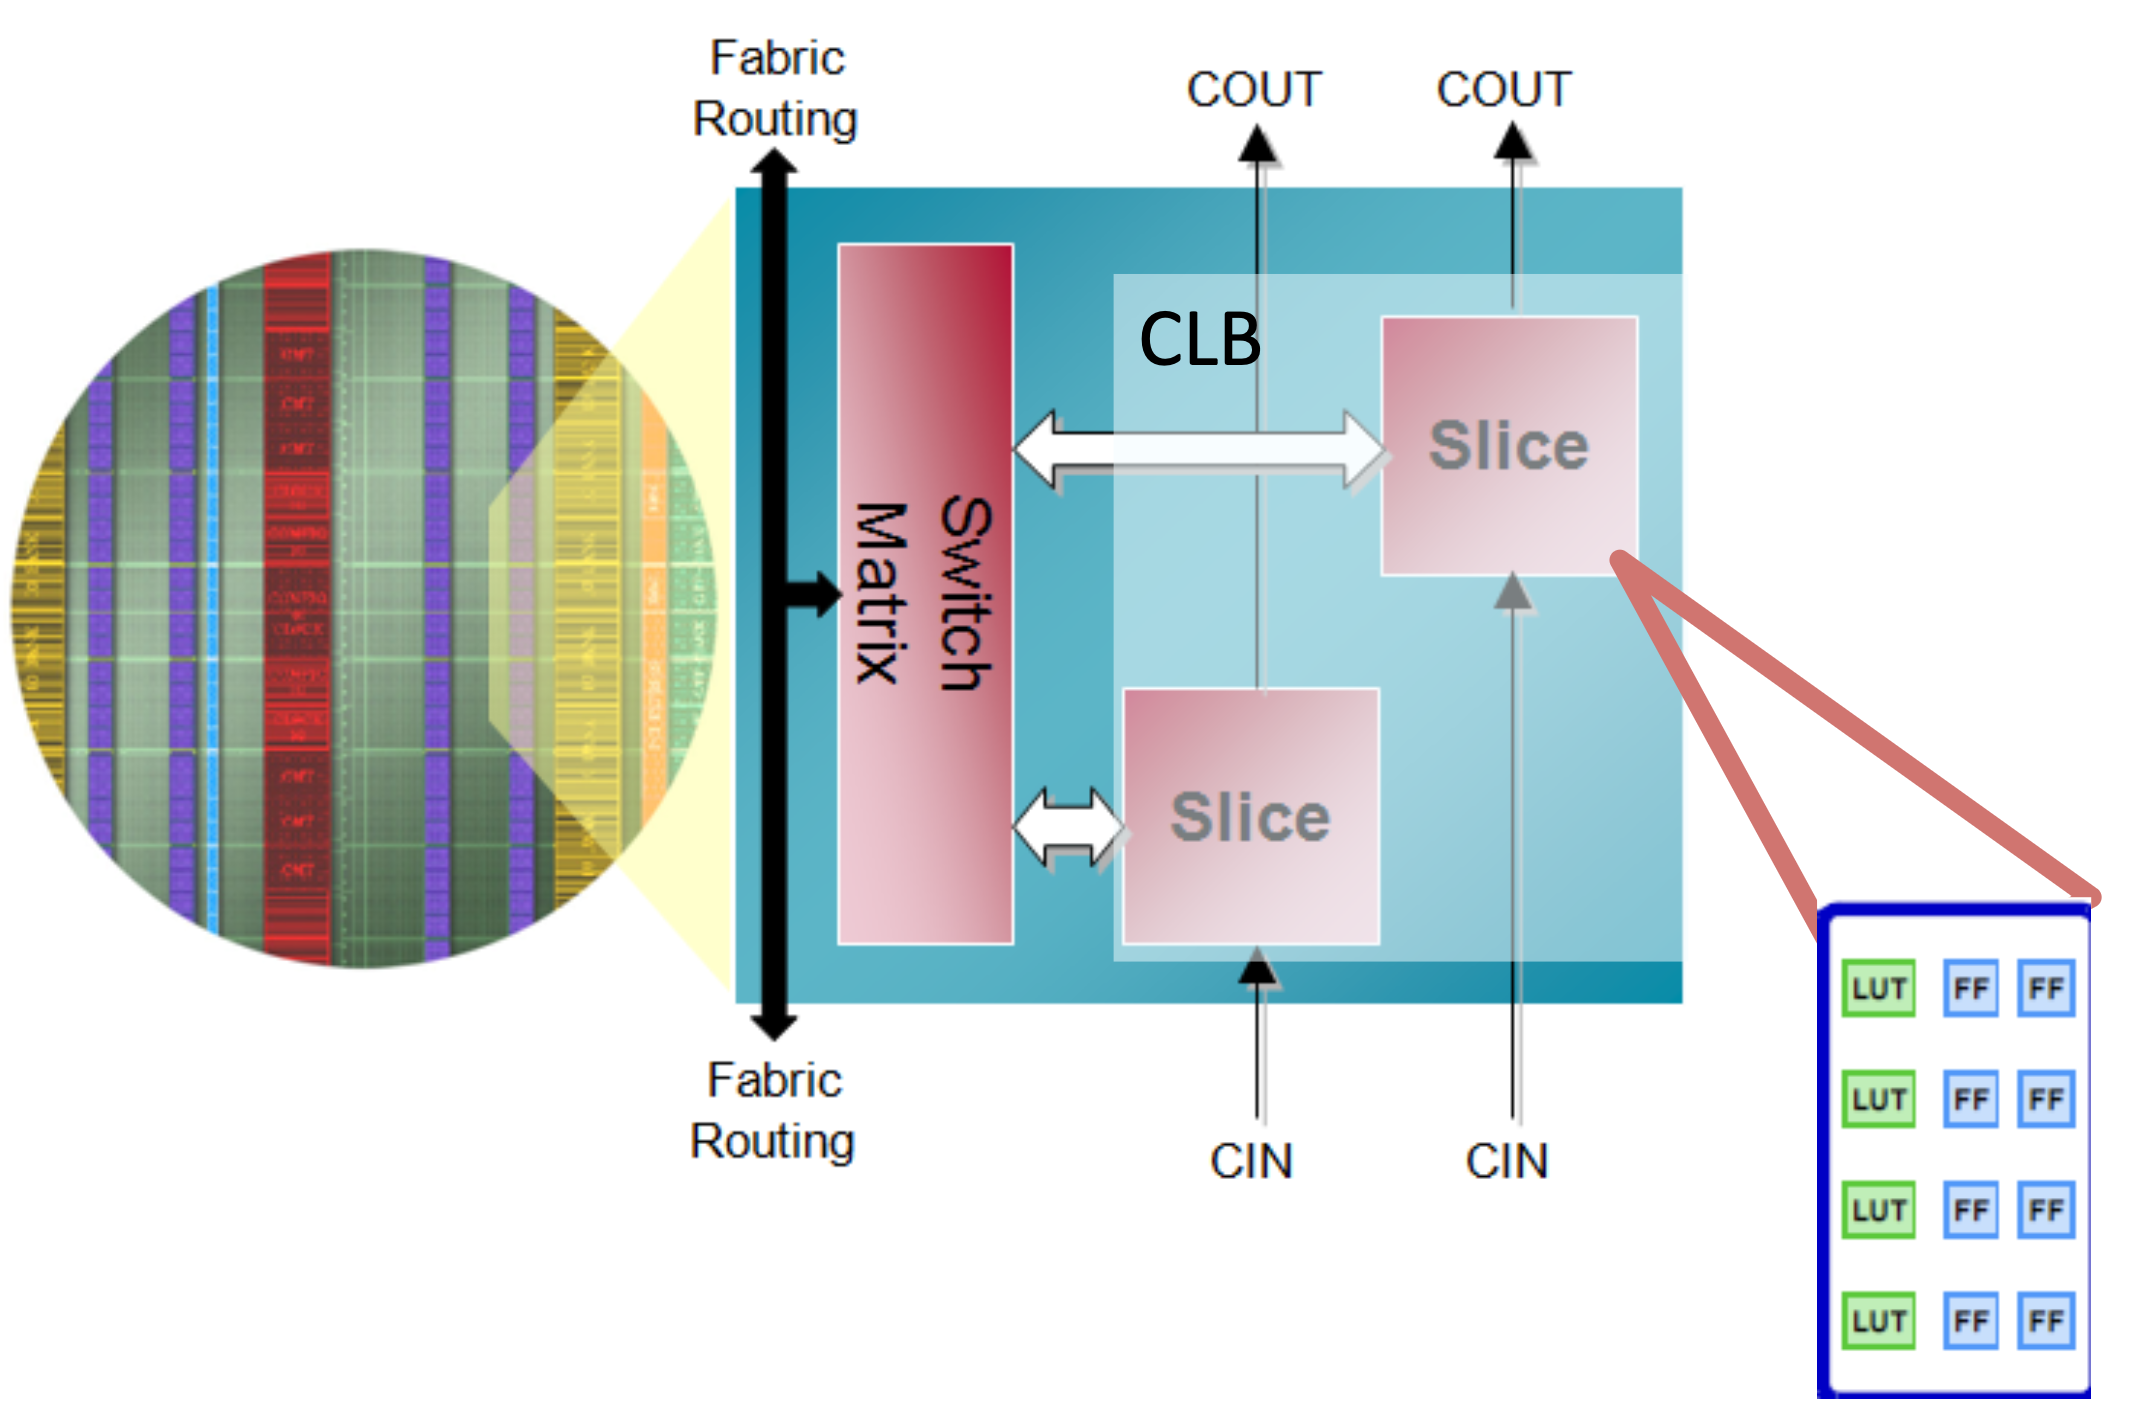
\includegraphics[width=\linewidth,height=0.28\textheight,keepaspectratio]{fig/L1_clb_slice.png}
  \caption{CLB- und Slice-Struktur der PL.}
\end{figure}

\subsection{I/O- und Analogressourcen}
Die 7-Series unterstützen High-Range- und High-Performance-I/Os mit LVDS, SERDES, Delay-Elementen und differenziellen Signalen. Ergänzend bietet das XADC-System integrierte ADCs und On-Chip-Sensorik für Mixed-Signal-Anwendungen.

\subsection{SoC-Design-Herausforderungen}
Zentrale Herausforderungen moderner SoC-Entwicklung:
\begin{itemize}
  \item Systemkomplexität und Parallelität
  \item Hardware/Software-Partitionierung
  \item Mehrere Clock-Domänen und Timing Closure
  \item IP-Integration und Wiederverwendbarkeit
  \item Team-basierte Entwicklungsflüsse
\end{itemize}

FPGA-Designs nähern sich methodisch ASIC-Plattformdesigns an.

\subsection{Design Flow und Tool-Unterstützung}
Der klassische RTL-zentrierte FPGA-Flow wird durch einen systemorientierten, IP-basierten Ansatz ergänzt. Kernelemente:
\begin{itemize}
  \item Abstraktionserhöhung
  \item HW/SW-Co-Design
  \item IP-Integration
  \item Einheitliches Constraint-System (XDC)
  \item Durchgängige Reports und Checkpoints
\end{itemize}

Vivado dient als zentrale Entwicklungsumgebung für Systemdesign, Implementierung, Analyse und Debugging.

\begin{figure}[t]
  \centering
  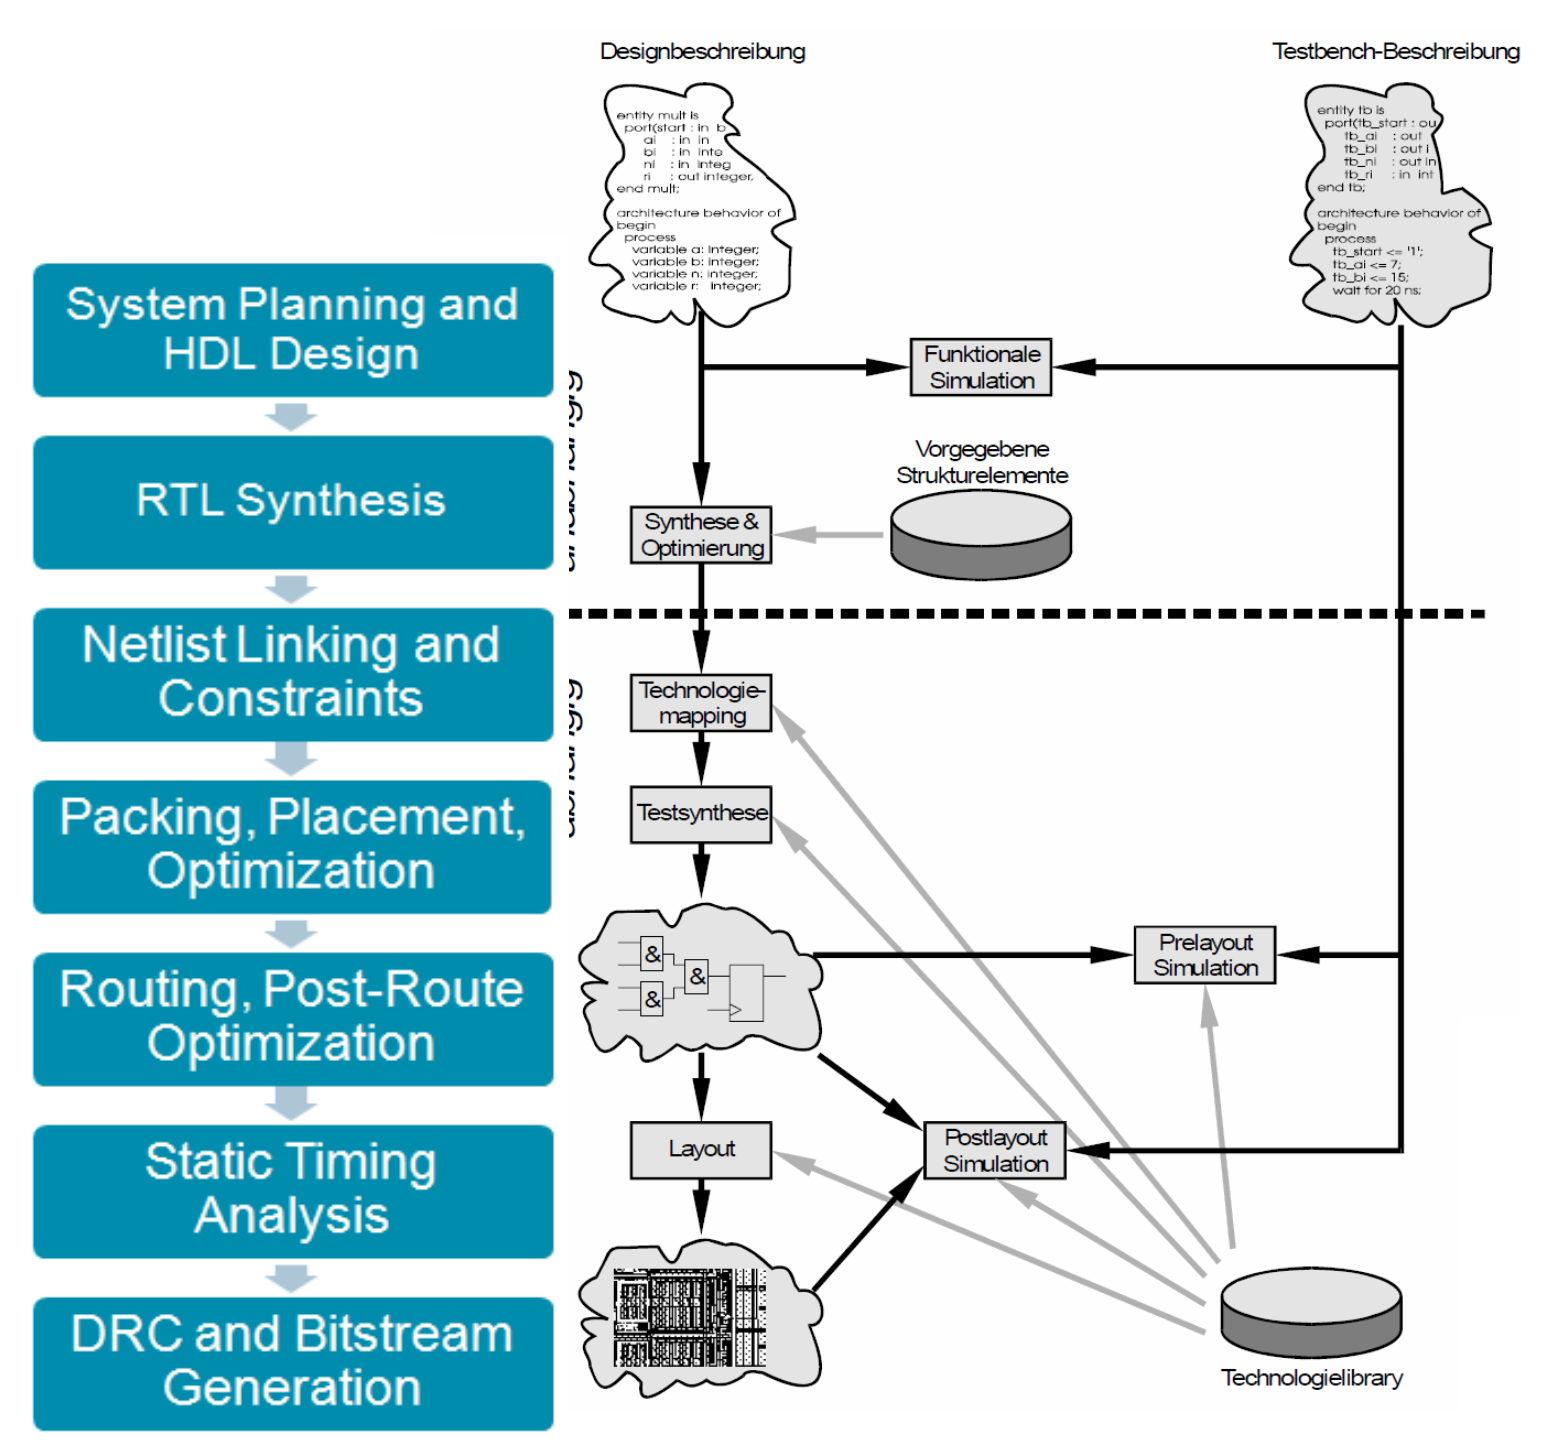
\includegraphics[width=\linewidth,height=0.28\textheight,keepaspectratio]{fig/L1_flow_rtl_vs_system.png}
  \caption{Traditioneller RTL/FPGA-Flow vs. System-Level/IP-Flow.}
\end{figure}

\begin{figure}[t]
  \centering
  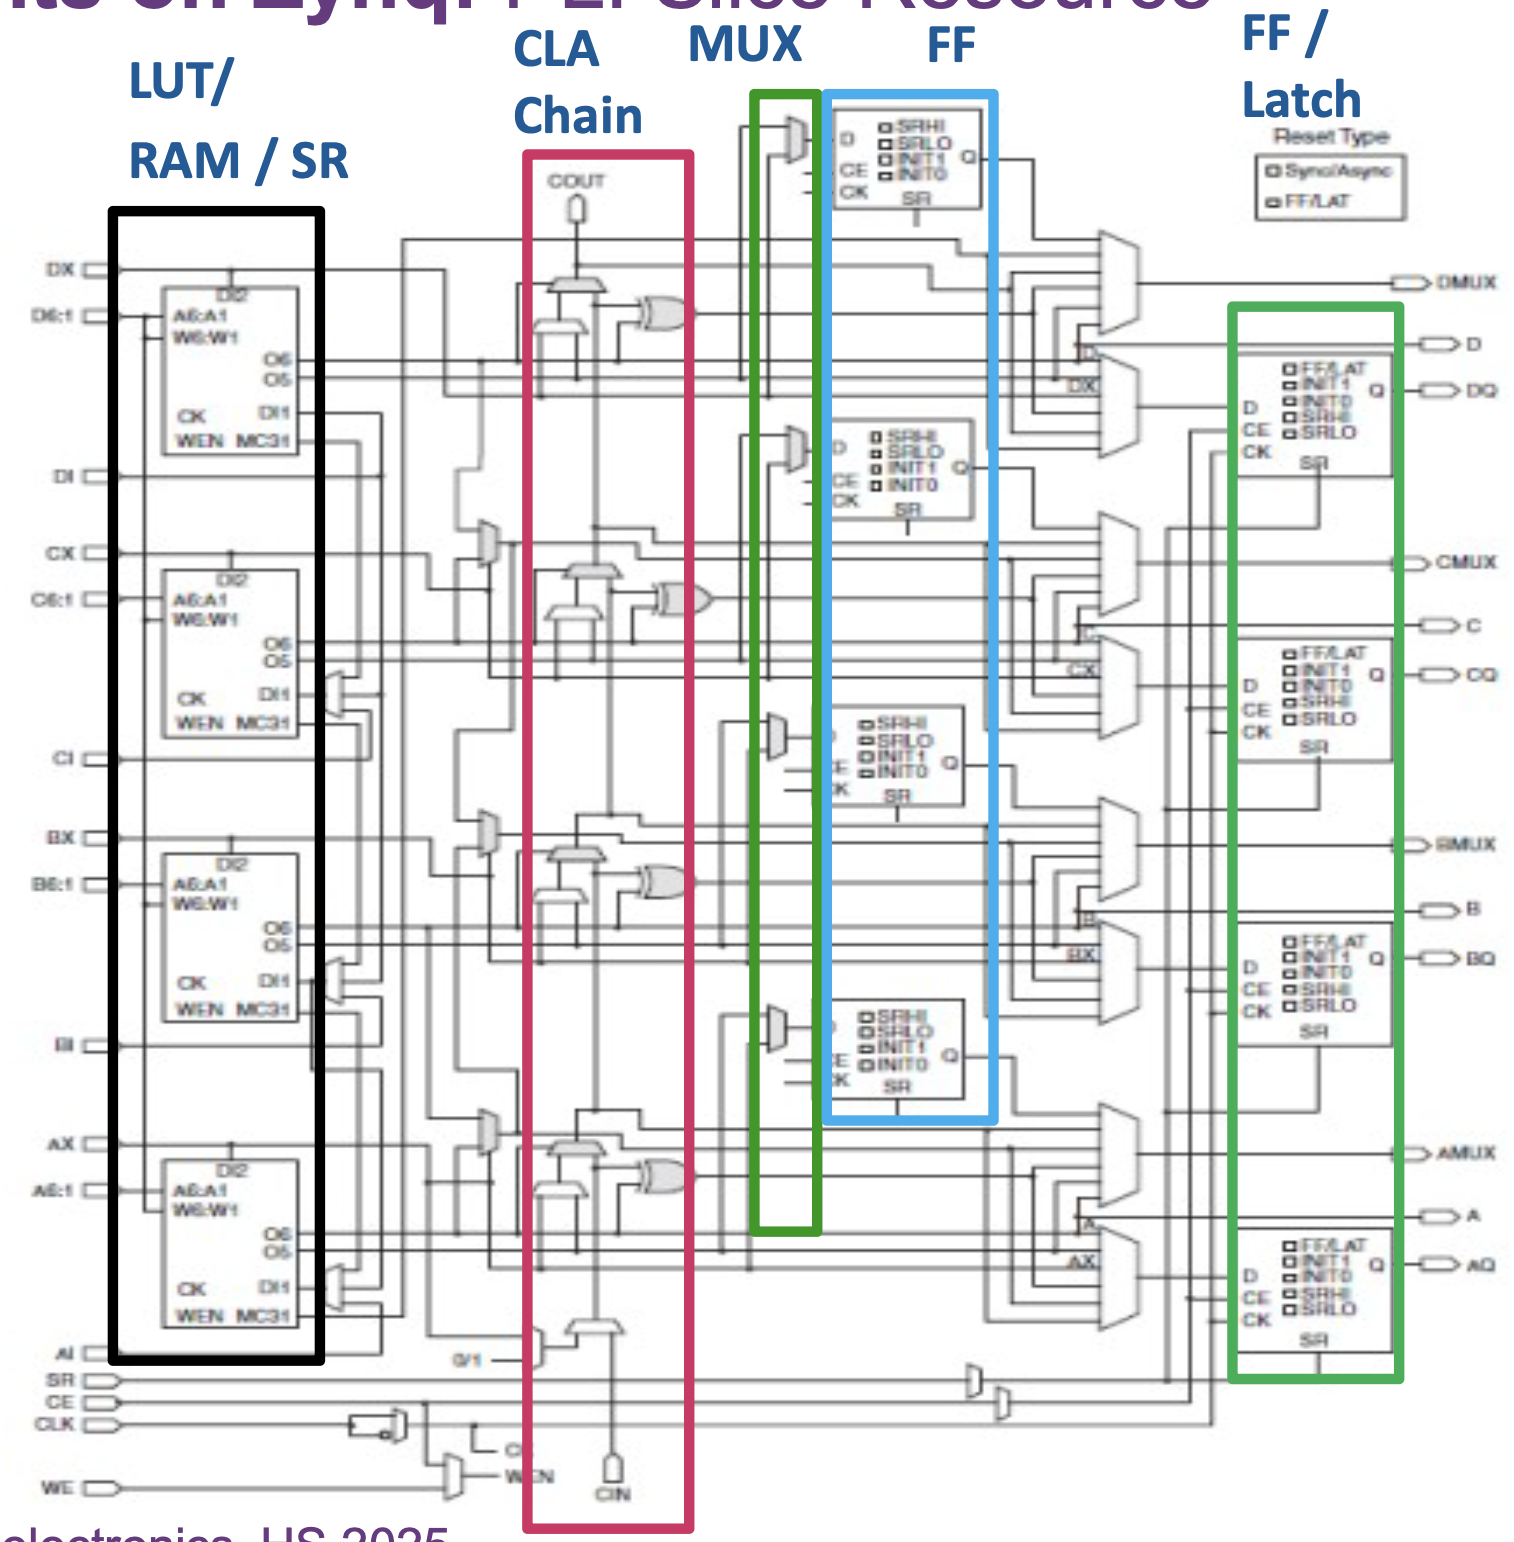
\includegraphics[width=\linewidth,height=0.24\textheight,keepaspectratio]{fig/L1_pld_fpga_soc.png}
  \caption{Entwicklung von PLD über FPGA zu SoC.}
\end{figure}



% ============================================================
\section{SoC Constraints}

\subsection{Rolle von Constraints im SoC-Design}
HDL beschreibt primär Funktionalität, nicht physikalische oder zeitliche Eigenschaften der Hardware.  
Moderne SoC-Designs sind ohne explizite Constraints nicht korrekt implementierbar.

\imp{Merksatz (Prüfung):}  
\hilite{Constraints} liefern dem Tool alle Informationen zu \textbf{Pins, \hilite{Spannungen} und \hilite{Zeiten}}, die im HDL fehlen.

Constraints steuern Synthese, Platzierung, Routing und Timing-Optimierung.

\subsection{Arten von Constraints}
Constraints lassen sich in drei Hauptkategorien einteilen:
\begin{itemize}
  \item \textbf{Physikalische Constraints:} Pin-Zuordnung, I/O-Standards, Nutzung spezifischer FPGA-Ressourcen, Platzierung von Zellen
  \item \textbf{Timing Constraints:} Clock-Definition, Input- und Output-Delays, Timing-Ausnahmen
  \item \textbf{Konfigurations-Constraints:} Bitstream-Optionen, Konfigurationsmodi
\end{itemize}

\imp{Prüfungsregel:}  
\hilite{Timing}-\hilite{Constraints} \hilite{wirken} bereits in der Synthese, physikalische Constraints primär in der Implementierung.

\subsection{XDC-Format und Constraint-Organisation}
Vivado verwendet XDC-Dateien auf Basis von Synopsys Design Constraints (SDC).  
Constraints folgen Tcl-Syntax und werden \textbf{sequentiell} interpretiert.

Empfohlene Struktur:
\begin{itemize}
  \item Timing Assertions (Clocks, I/O-Delays)
  \item Timing Exceptions (False Paths, Multicycle Paths)
  \item Physikalische Constraints (Pins, I/O-Standards)
\end{itemize}

\textbf{Merksatz:}  
\hilite{Timing zuerst, Pins zuletzt.}

\subsection{Physikalische Constraints}
Physikalische Constraints definieren die Abbildung logischer Ports auf physische Pins sowie elektrische Eigenschaften:
\begin{itemize}
  \item Pin-Zuweisung (\texttt{PACKAGE\_PIN})
  \item I/O-Standard (\texttt{IOSTANDARD})
  \item Pull-Ups, Pull-Downs
\end{itemize}

\subsubsection*{\textcolor{codeemph}{Vorgehensschema (Prüfung)}}
\begin{enumerate}
  \item Signalrichtung bestimmen
  \item Spannung bestimmen $\rightarrow$ \texttt{IOSTANDARD}
  \item Pin zuordnen $\rightarrow$ \texttt{PACKAGE\_PIN}
  \item Reset? $\rightarrow$ \texttt{PULLUP true}
\end{enumerate}

\subsubsection*{XDC-Code-Schablone}
\begin{lstlisting}[style=xdc,emph={set_property,get_ports,PACKAGE_PIN,IOSTANDARD,PULLUP},emphstyle=\bfseries\color{codeemph}]
set_property IOSTANDARD LVCMOS33 [get_ports rst]
set_property PULLUP true [get_ports rst]
set_property PACKAGE_PIN V13 [get_ports rst]
\end{lstlisting}

In Sonderfällen können explizite Platzierungsconstraints (\texttt{LOC}, \texttt{BEL}) verwendet werden.

\subsection{Timing-Grundlagen und Begriffe}
Timing-Verifikation erfolgt mittels Static Timing Analysis (STA).

Zentrale Begriffe:
\begin{itemize}
  \item \textbf{Clock Latency}
  \item \textbf{Clock Skew}
  \item \textbf{Clock Jitter}
  \item \textbf{Slack}
\end{itemize}

\imp{Prüfungsregel:}  
\hilite{Timing} ist korrekt, wenn \hilite{Setup}- und Hold-Bedingungen erfüllt sind und der \hilite{Slack $\ge 0$} ist.

\begin{figure}[t]
  \centering
  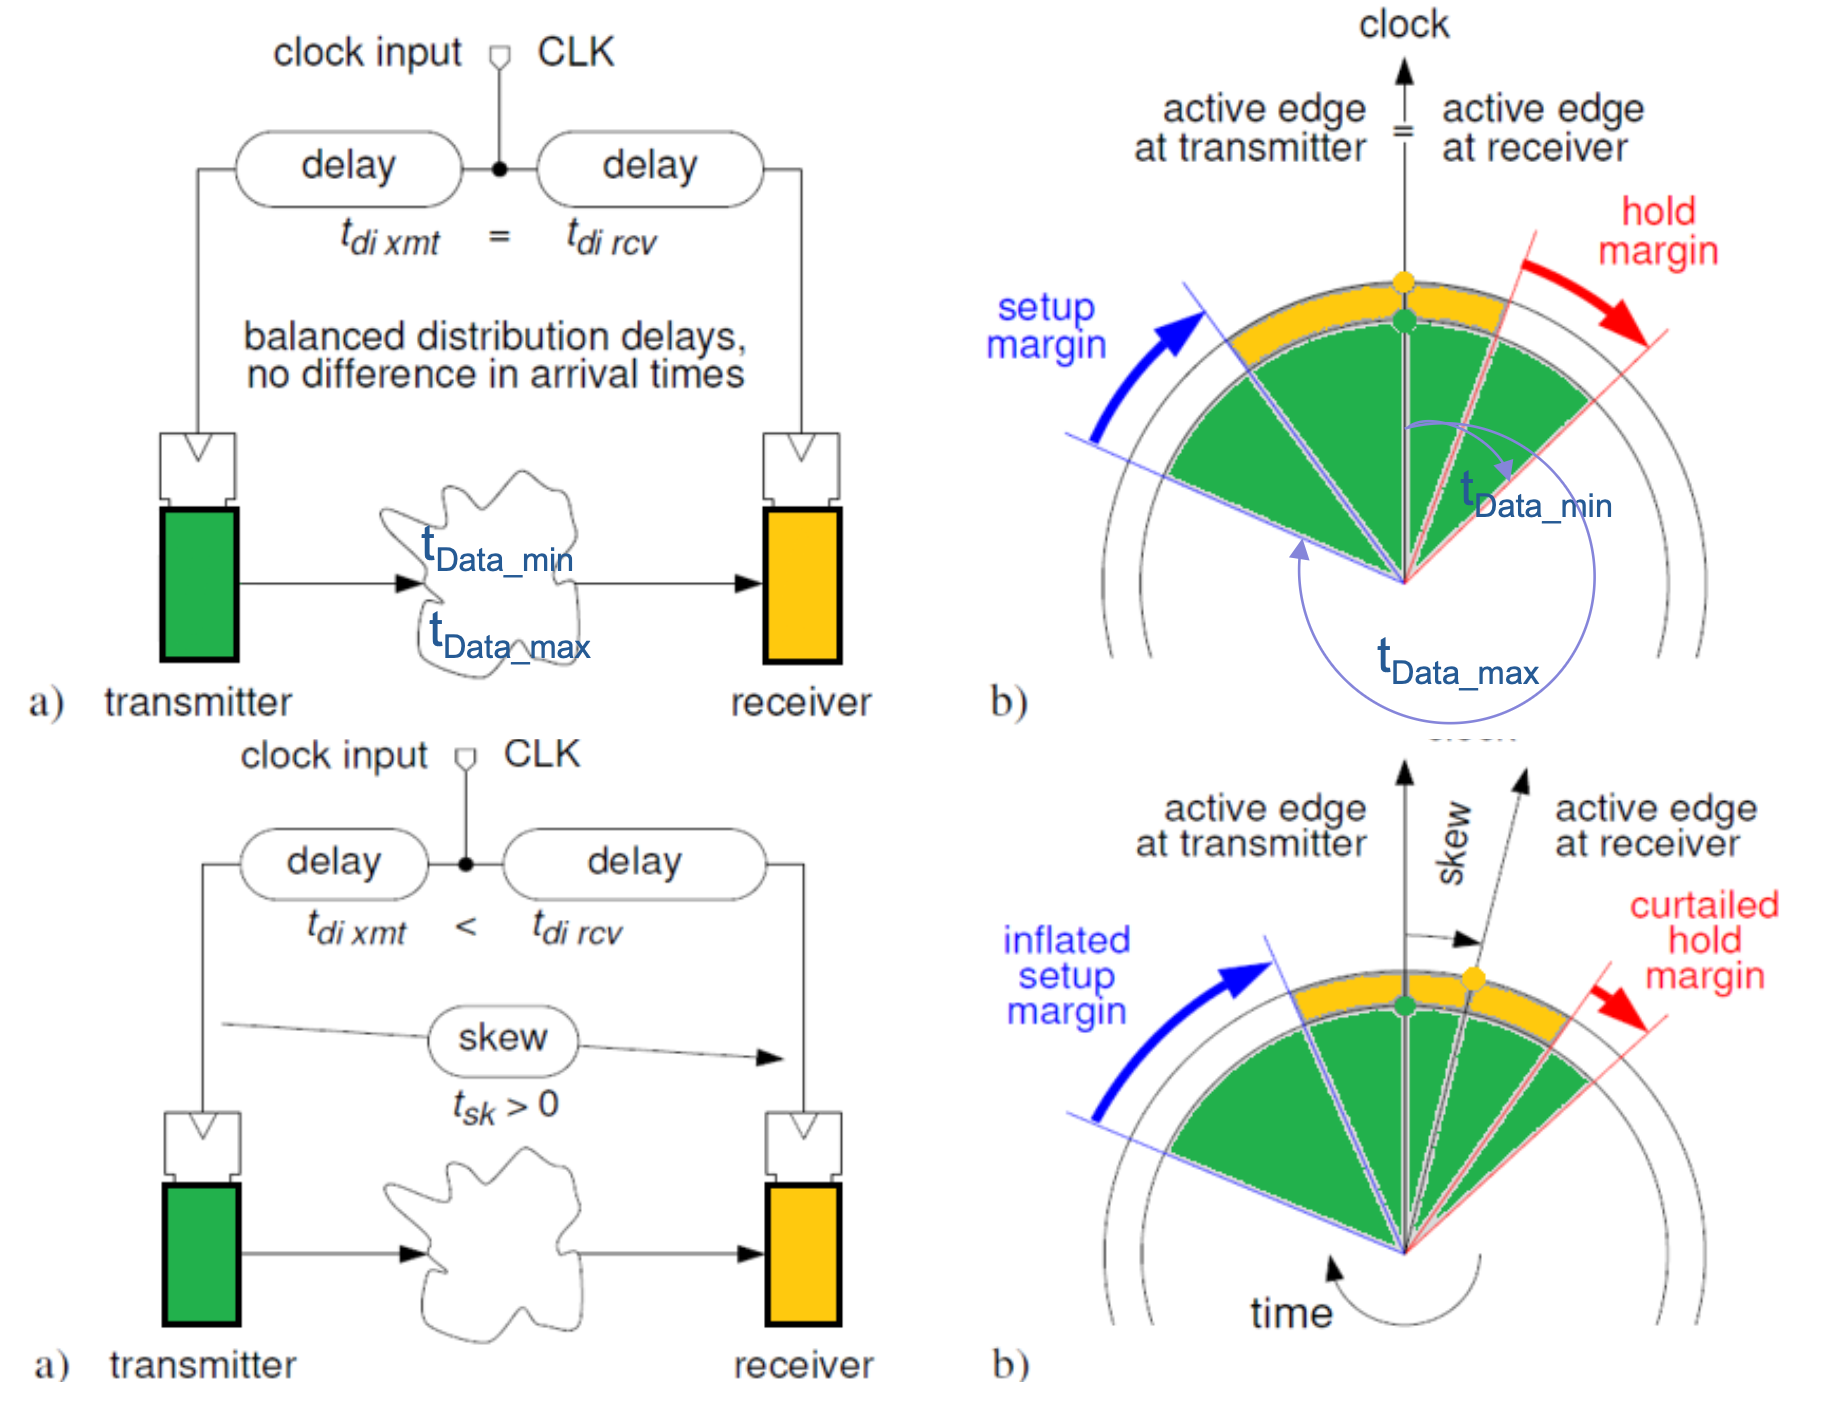
\includegraphics[width=\linewidth,height=0.26\textheight,keepaspectratio]{fig/L2_clock_skew.png}
  \caption{Timing-Nichtidealitäten: Latency, Skew und Jitter.}
\end{figure}

\subsection{Static Timing Analysis (STA)}
STA analysiert alle relevanten Minimal- und Maximalpfade ohne Simulation:
\begin{itemize}
  \item Clock-to-Clock-Pfade
  \item Setup-, Hold- und Pulse-Width-Bedingungen
\end{itemize}

Wichtige Kennzahlen:
\begin{itemize}
  \item Worst Negative Slack (WNS)
  \item Total Negative Slack (TNS)
\end{itemize}

\subsection{Clock-Definition}
Jede relevante Clock muss explizit definiert werden.

\subsubsection*{Formel}
\[
T_{clk} = \frac{1}{f}
\]

\subsubsection*{Code-Schablone}
\begin{lstlisting}[emph={entity,architecture,process,rising_edge,signal,constant,generic,port},emphstyle=\bfseries\color{codeemph}][emph={entity,architecture,process,rising_edge,signal,constant,generic,port},emphstyle=\bfseries\color{codeemph}]
create_clock -name clk -period 10 [get_ports clk]
\end{lstlisting}

\subsection{Input-Delay-Constraints}
Externe Signalankunftszeiten müssen spezifiziert werden.

\subsubsection*{\textcolor{codeemph}{Prüfungsformel}}
\[
t_{input\_delay} = t_{data} - t_{clk}
\]

\subsubsection*{Code-Schablone}
\begin{lstlisting}[emph={entity,architecture,process,rising_edge,signal,constant,generic,port},emphstyle=\bfseries\color{codeemph}]
set_input_delay -clock clk 3 [get_ports data_in]
\end{lstlisting}

\subsection{Output-Delay-Constraints}
Output-Delays definieren erforderliche externe Setup- und Hold-Zeiten.

\subsubsection*{Code-Schablone}
\begin{lstlisting}[emph={entity,architecture,process,rising_edge,signal,constant,generic,port},emphstyle=\bfseries\color{codeemph}][emph={entity,architecture,process,rising_edge,signal,constant,generic,port},emphstyle=\bfseries\color{codeemph}]
set_output_delay -clock clk 5 [get_ports data_out]
\end{lstlisting}

\begin{figure}[t]
  \centering
  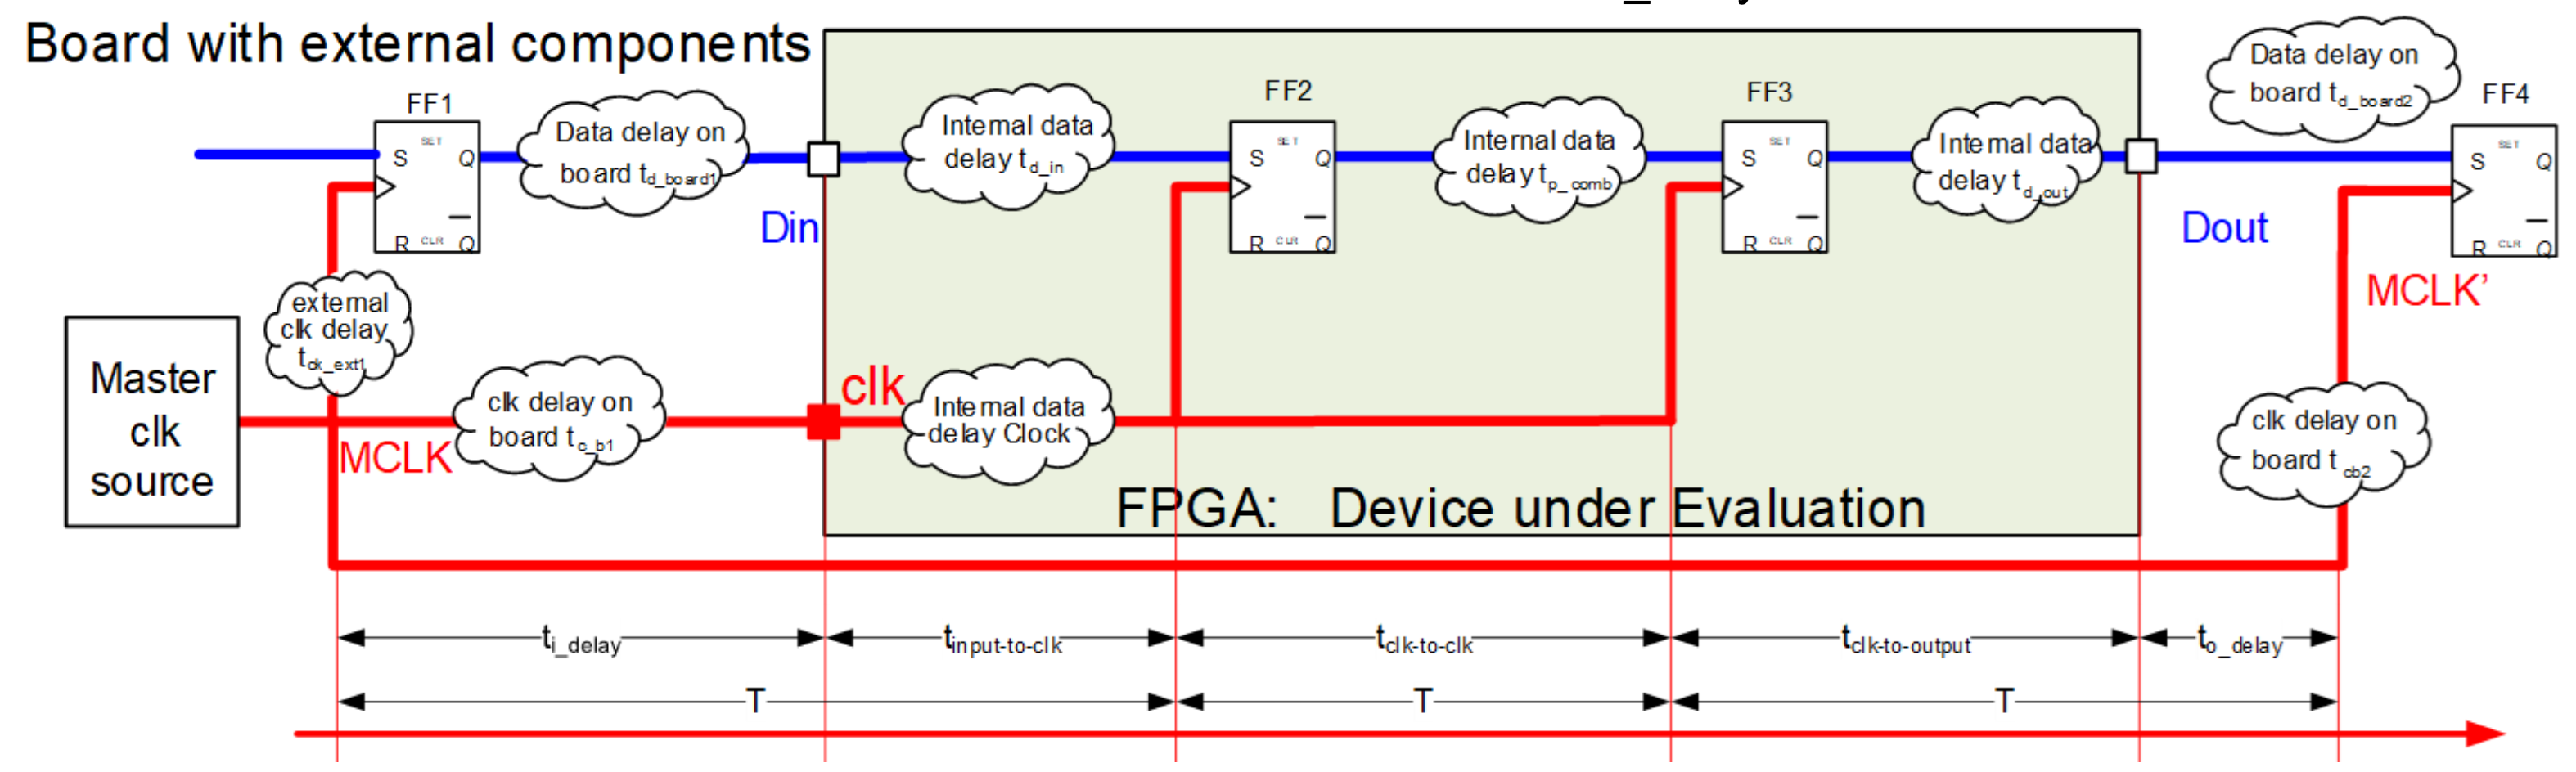
\includegraphics[width=\linewidth,height=0.26\textheight,keepaspectratio]{fig/L2_io_delays.png}
  \caption{Input- und Output-Delay-Pfade mit externen Komponenten.}
\end{figure}

\subsection{Wirkung von Constraints}
Constraints beeinflussen Platzierung, Routing und Optimierung direkt.

\imp{Abschluss-Merksatz (Prüfung):}  
Ohne korrekte \hilite{Constraints} kein valides Timing und kein reproduzierbares Design.

% ============================================================
\section{\hilite{System Level VHDL} und IP-\hilite{Wiederverwendung}}

\subsection{Zielsetzung von System Level VHDL}
Moderne SoC-Entwicklung erfordert skalierbare, parametrisierbare und wiederverwendbare Hardwarebeschreibungen. System Level VHDL adressiert Komplexität, Heterogenität und Time-to-Market durch Hierarchie, Modularisierung und Abstraktion.

\imp{Merksatz (Prüfung):}  
\hilite{System Level VHDL} zielt auf \textbf{\hilite{Wiederverwendung} und \hilite{Skalierung}}, nicht auf Gate-Optimierung.

Ziel ist die Wiederverwendung bewährter IP-Blöcke statt monolithischer, hardcodierter Designs.

\subsection{Grundprinzipien der Wiederverwendung}
Wiederverwendbarer VHDL-Code folgt klaren Regeln:
\begin{itemize}
  \item Keine fest kodierten Parameter
  \item Klare Schnittstellen
  \item Parametrisierung über Generics
  \item Zentrale Definition von Konstanten und Typen
  \item Saubere Dokumentation und Kommentare
\end{itemize}

\imp{Prüfungsregel:}  
\hilite{Projektweit} konstant $\Rightarrow$ \hilite{Package}. Variabel pro Instanz $\Rightarrow$ \hilite{Generic}.

Code wird typischerweise von anderen Entwicklern genutzt als vom ursprünglichen Autor. Lesbarkeit ist ein funktionales Kriterium.

\subsection{Alias, Konstanten und Generics}
Aliases verbessern die Lesbarkeit, insbesondere bei Vektorslices.

\subsubsection*{Alias – Code-Schablone}
\begin{lstlisting}[emph={entity,architecture,process,rising_edge,signal,constant,generic,port},emphstyle=\bfseries\color{codeemph}]
alias opcode : std_logic_vector(3 downto 0) is instr(15 downto 12);
\end{lstlisting}

Konstanten definieren unveränderliche Entwurfsparameter und erhöhen Konsistenz.

\subsubsection*{Konstante – Code-Schablone}
\begin{lstlisting}[emph={entity,architecture,process,rising_edge,signal,constant,generic,port},emphstyle=\bfseries\color{codeemph}][emph={entity,architecture,process,rising_edge,signal,constant,generic,port},emphstyle=\bfseries\color{codeemph}]
constant DATA_WIDTH : integer := 16;
\end{lstlisting}

Generics ermöglichen die Übergabe statischer Parameter von außen in eine Entity.

\subsubsection*{Generic – Code-Schablone}
\begin{lstlisting}[emph={entity,architecture,process,rising_edge,signal,constant,generic,port},emphstyle=\bfseries\color{codeemph}]
entity alu is
  generic ( WIDTH : integer := 16 );
  port (
    a, b : in  std_logic_vector(WIDTH-1 downto 0);
    y    : out std_logic_vector(WIDTH-1 downto 0)
  );
end entity;
\end{lstlisting}

\textbf{Merksatz:}  
\hilite{Generics} werden bei der \hilite{Instanziierung} \hilite{festgelegt} und sind zur Laufzeit konstant.

\subsection{Generate-Konstrukte}
Generate-Anweisungen erlauben die strukturierte Erzeugung mehrfacher Instanzen. In Kombination mit Generics entstehen skalierbare Hardwarestrukturen.

Typische Einsatzfälle:
\begin{itemize}
  \item Replikation identischer Verarbeitungseinheiten
  \item Parametrisierbare Breiten und Tiefen
  \item Strukturierte Arrays von Modulen
\end{itemize}

\imp{Prüfungsregel:}  
\hilite{Generate} ist \hilite{elaborationszeitlich} \hilite{wirksam} und erzeugt \textbf{echte Hardware}.

\subsubsection*{Generate – Code-Schablone}
\begin{lstlisting}[emph={entity,architecture,process,rising_edge,signal,constant,generic,port},emphstyle=\bfseries\color{codeemph}][emph={entity,architecture,process,rising_edge,signal,constant,generic,port},emphstyle=\bfseries\color{codeemph}]
gen_loop : for i in 0 to N-1 generate
  u : entity work.reg
    port map (clk => clk, d => din(i), q => dout(i));
end generate;
\end{lstlisting}

\begin{figure}[t]
  \centering
  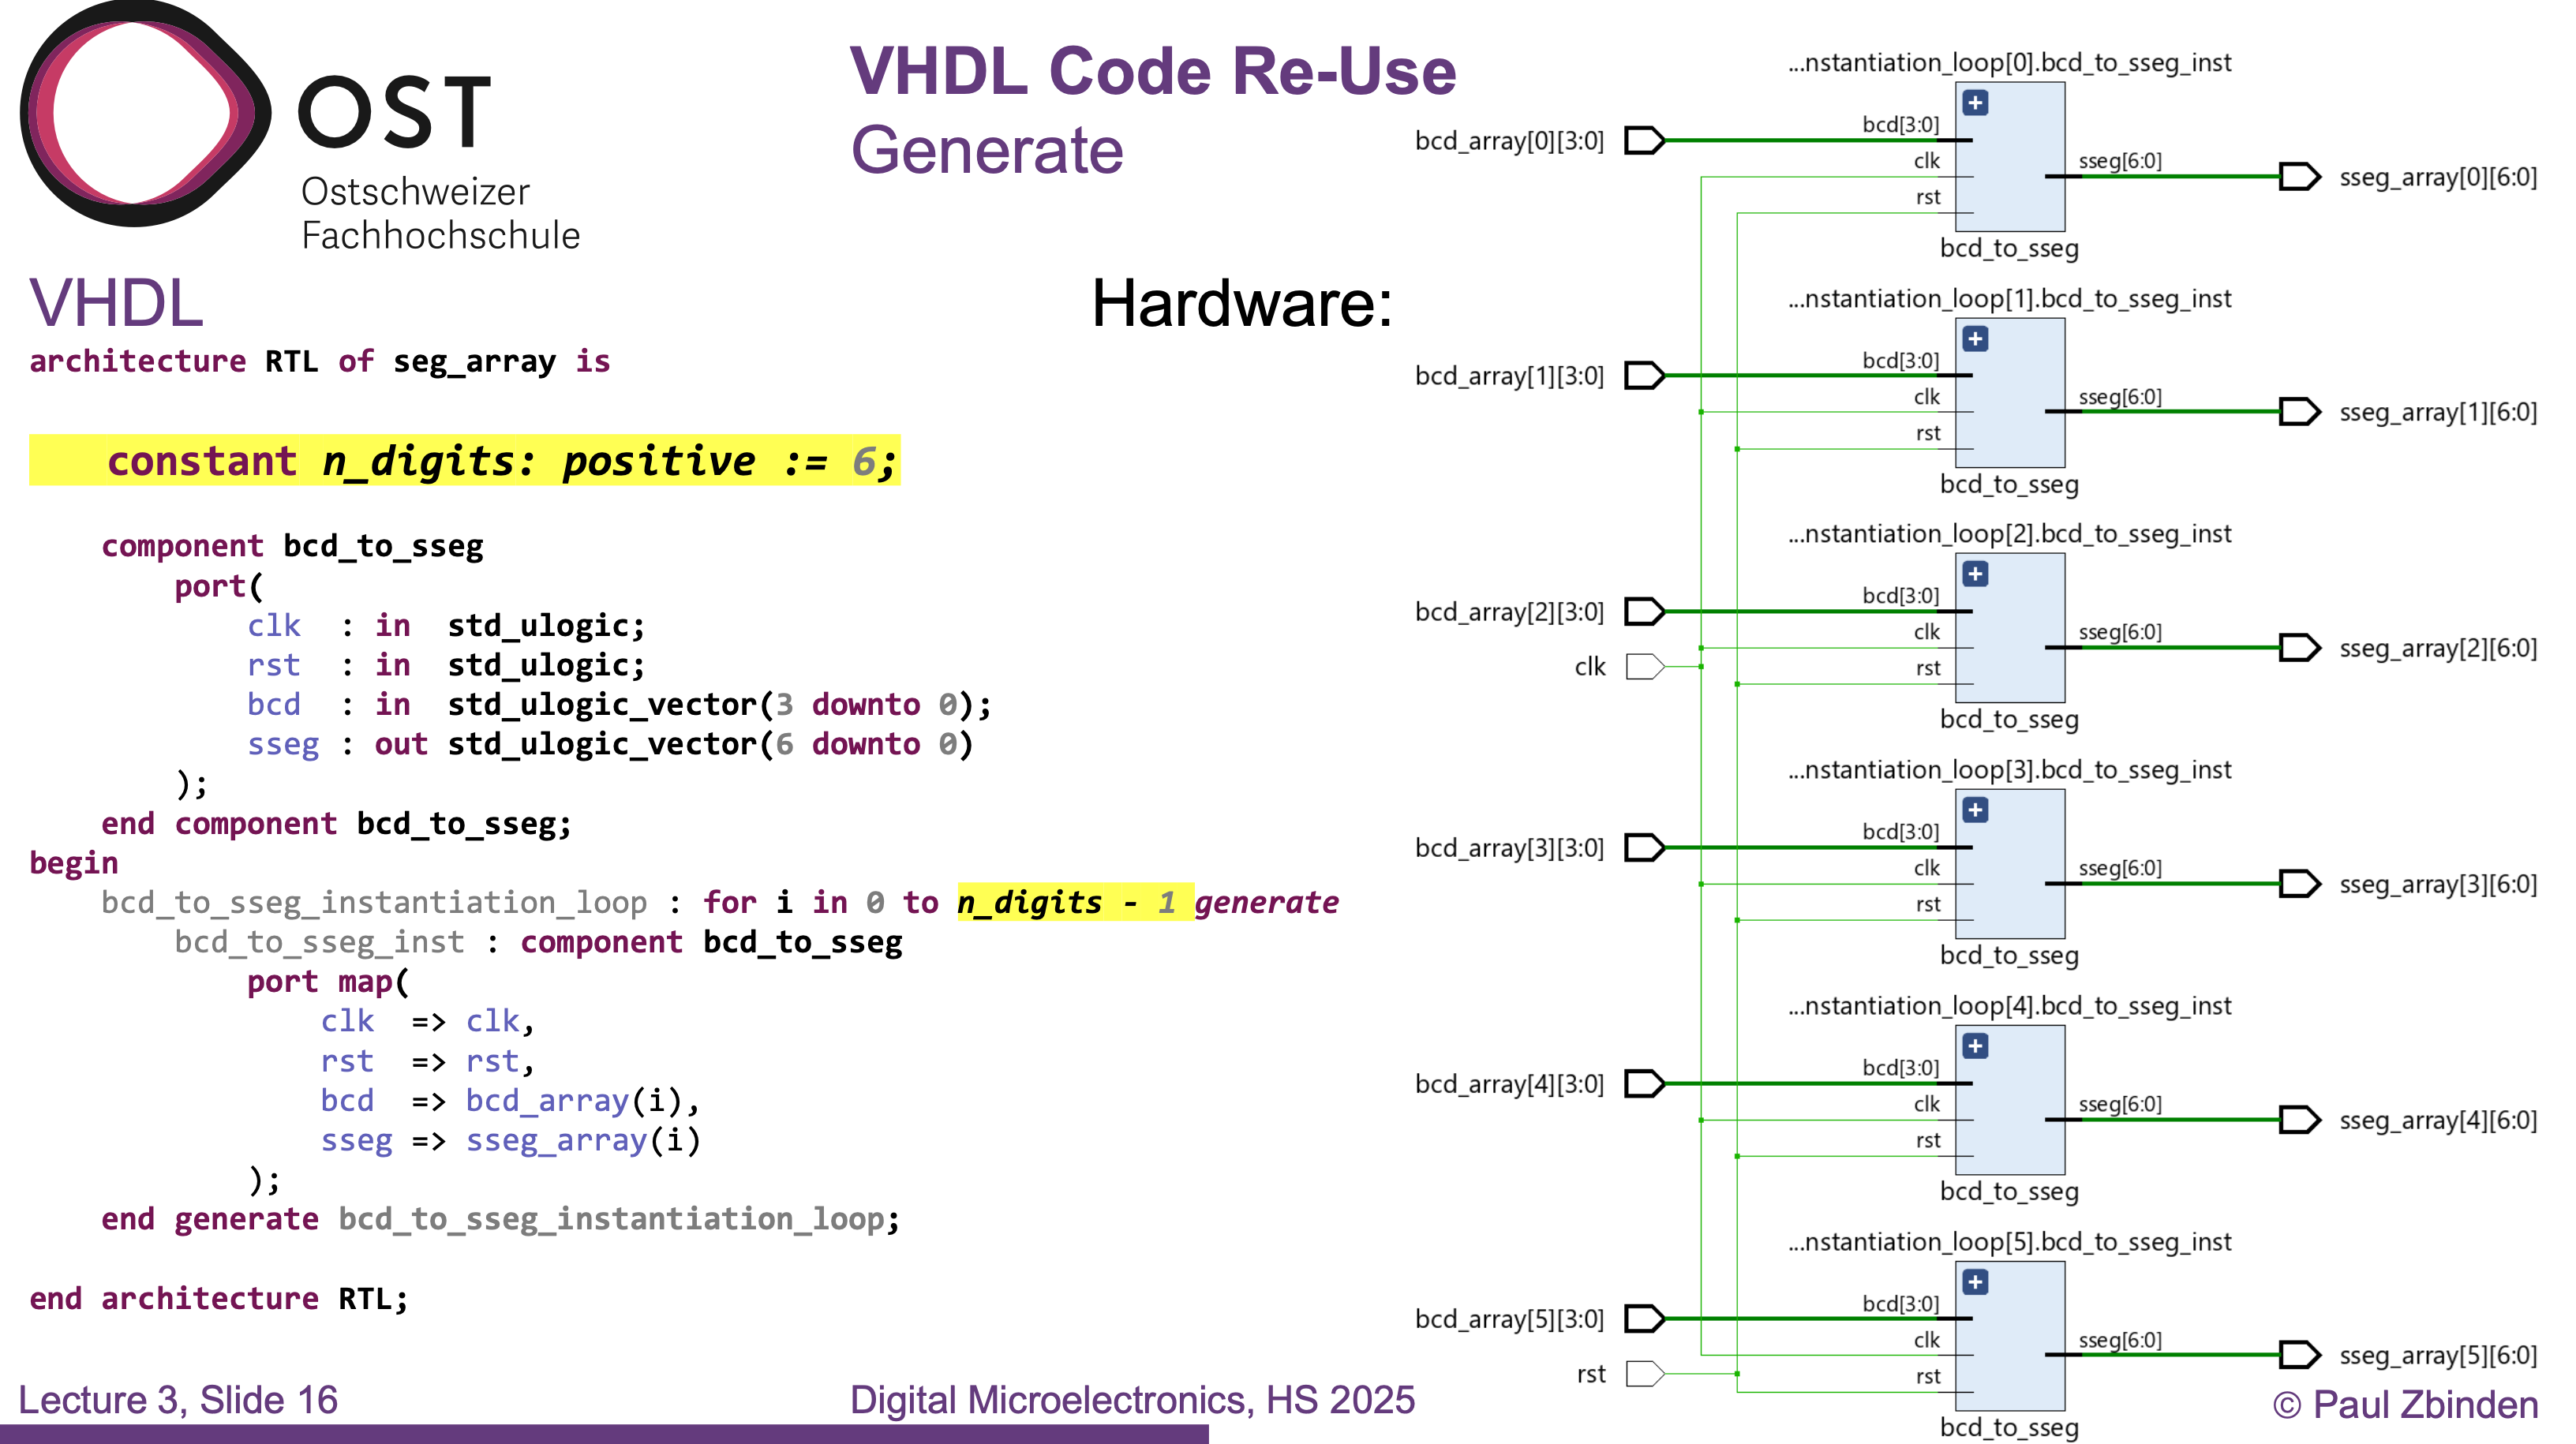
\includegraphics[width=\linewidth,height=0.26\textheight,keepaspectratio]{fig/L3_generate_structure.png}
  \caption{Generate-Struktur und resultierende Hardware.}
\end{figure}

\subsection{Funktionen in VHDL}
Funktionen sind nebenläufig nutzbare Unterprogramme mit ausschließlich Eingangsparametern und genau einem Rückgabewert. Sie werden wie Ausdrücke verwendet und dienen der strukturellen Abstraktion.

Eigenschaften:
\begin{itemize}
  \item Keine Signalzuweisungen
  \item Keine Wait-Statements
  \item Verwendung von Variablen
  \item Rekursion erlaubt
\end{itemize}

\subsubsection*{Funktion – Code-Schablone}
\begin{lstlisting}[emph={entity,architecture,process,rising_edge,signal,constant,generic,port},emphstyle=\bfseries\color{codeemph}]
function max(a,b : integer) return integer is
begin
  if a > b then return a; else return b; end if;
end function;
\end{lstlisting}

Funktionen eignen sich besonders für kombinatorische Logik und arithmetische Operationen.

\subsection{Prozeduren in VHDL}
Prozeduren können mehrere Ein- und Ausgänge besitzen. Sie sind mächtiger als Funktionen, jedoch eingeschränkt synthesefähig. Hauptanwendungsgebiet sind Testbenches und Verhaltensmodelle.

\imp{Prüfungsregel:}  
\hilite{Prozeduren} in \hilite{Synthese} sind \hilite{toolabhängig} und kritisch zu prüfen.

\subsection{Arrays und Records}
Arrays modellieren Sammlungen gleichartiger Elemente. Sie können eindimensional oder mehrdimensional sein und sowohl natürliche als auch enumerierte Indizes verwenden.

\subsubsection*{Array – Code-Schablone}
\begin{lstlisting}[emph={entity,architecture,process,rising_edge,signal,constant,generic,port},emphstyle=\bfseries\color{codeemph}][emph={entity,architecture,process,rising_edge,signal,constant,generic,port},emphstyle=\bfseries\color{codeemph}]
type vec_t is array (0 to 7) of std_logic_vector(15 downto 0);
signal v : vec_t;
\end{lstlisting}

Records gruppieren Elemente unterschiedlicher Typen zu logischen Strukturen. Sie eignen sich für Busse, Transaktionen und strukturierte Datensätze im Systementwurf.

\subsubsection*{Record – Code-Schablone}
\begin{lstlisting}[emph={entity,architecture,process,rising_edge,signal,constant,generic,port},emphstyle=\bfseries\color{codeemph}]
type bus_t is record
  addr : std_logic_vector(15 downto 0);
  data : std_logic_vector(31 downto 0);
  we   : std_logic;
end record;
\end{lstlisting}

\begin{figure}[t]
  \centering
  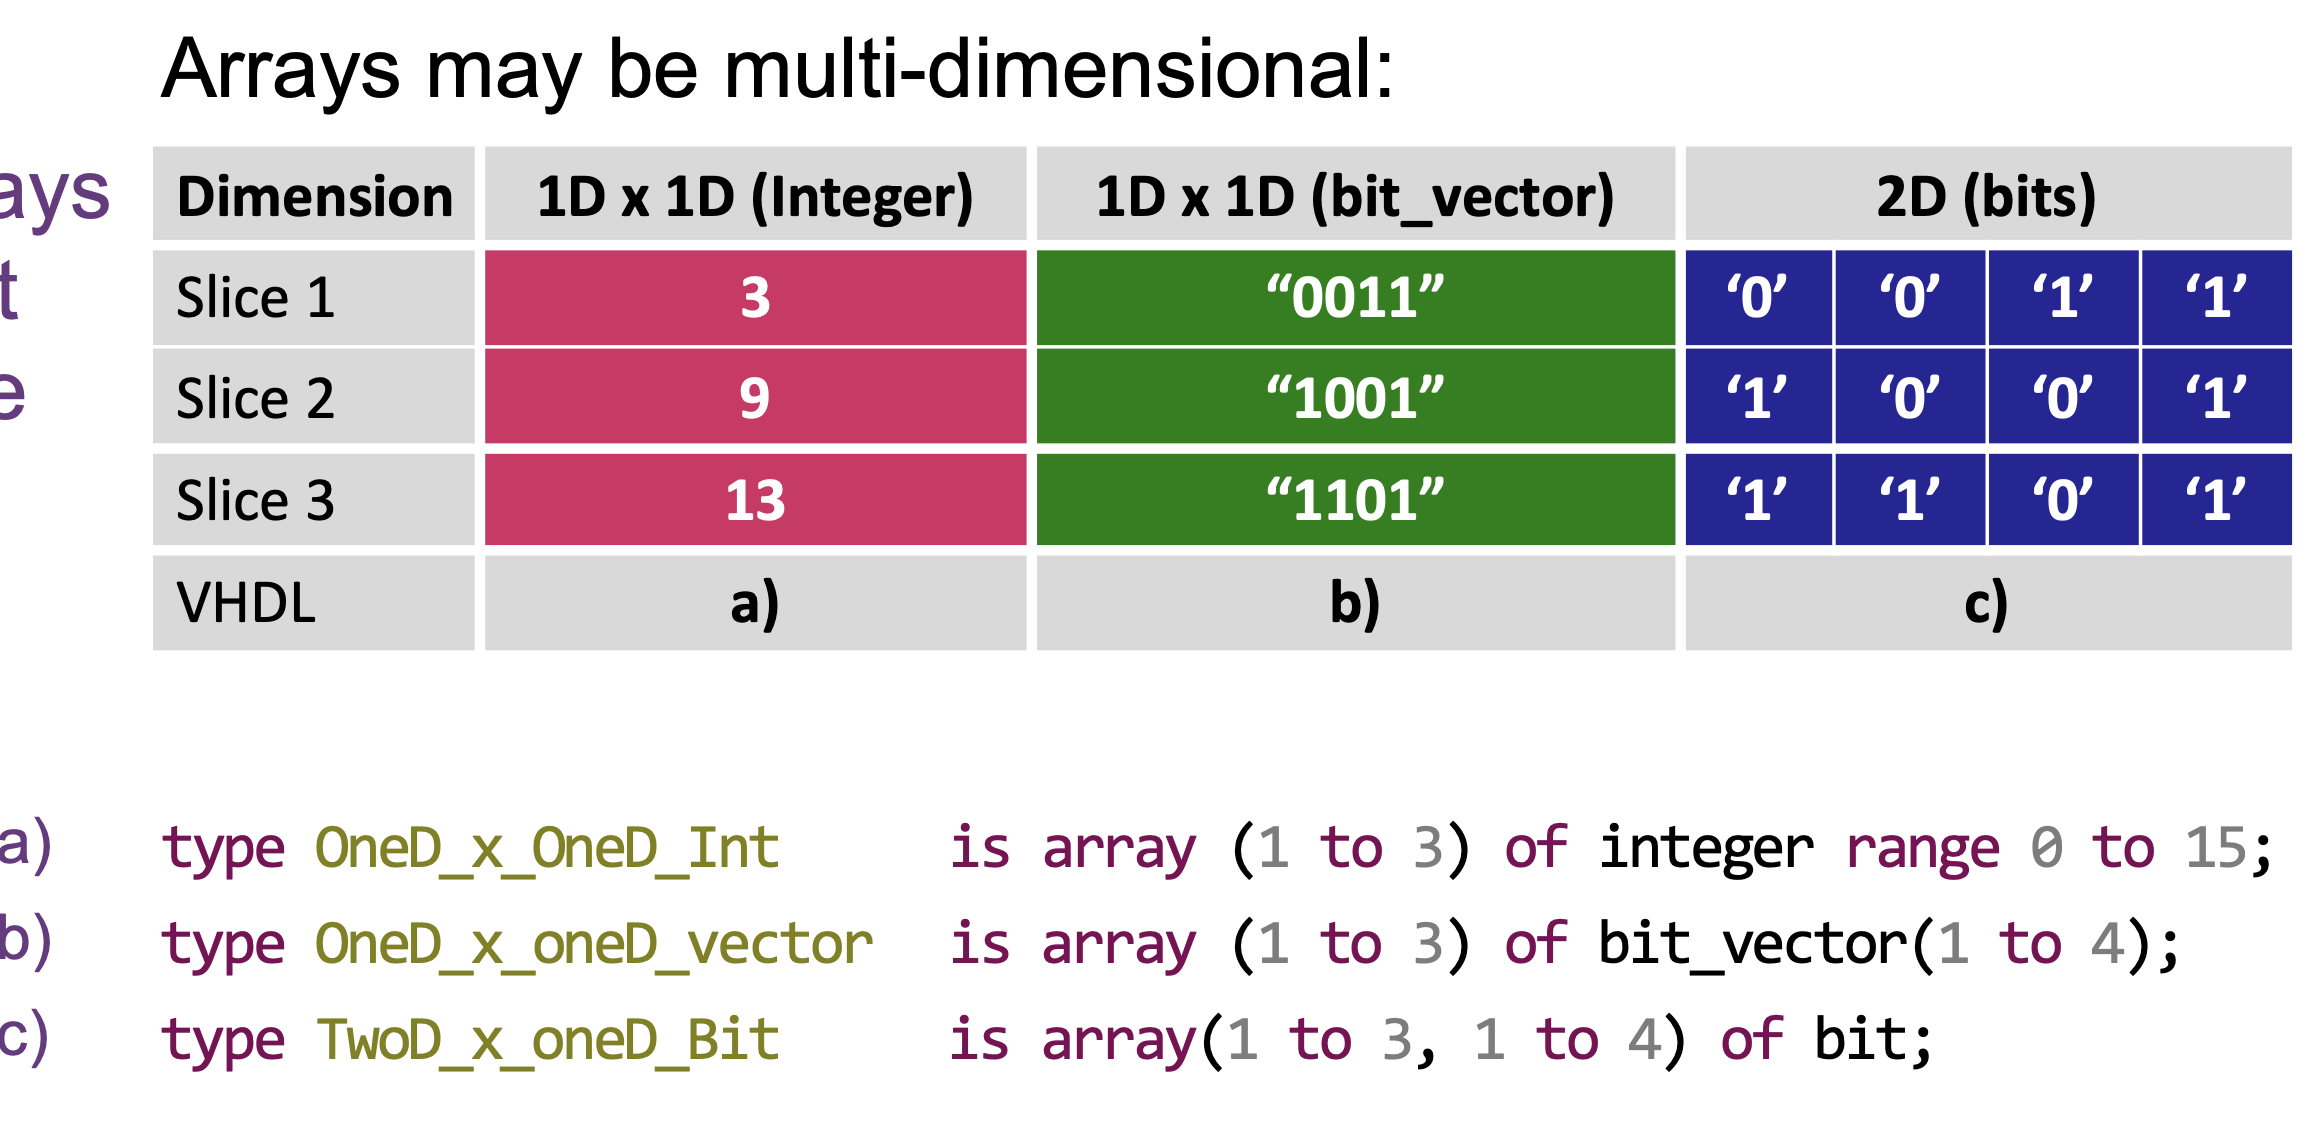
\includegraphics[width=\linewidth,height=0.26\textheight,keepaspectratio]{fig/L3_array_record.png}
  \caption{Array- und Record-Beispiele mit Hardwareabbildung.}
\end{figure}

\subsection{Packages}
Packages sind zentrale Container für projektweite Definitionen:
\begin{itemize}
  \item Konstanten
  \item Typen
  \item Komponenten
  \item Funktionen und Prozeduren
\end{itemize}

Sie fördern Konsistenz, Wiederverwendung und Wartbarkeit. Packages werden kompiliert in Libraries abgelegt und über \texttt{use}-Anweisungen eingebunden.

\subsubsection*{Package – Minimal-Schablone}
\begin{lstlisting}[emph={entity,architecture,process,rising_edge,signal,constant,generic,port},emphstyle=\bfseries\color{codeemph}][emph={entity,architecture,process,rising_edge,signal,constant,generic,port},emphstyle=\bfseries\color{codeemph}]
package defs is
  constant WIDTH : integer := 16;
  function inc(x : integer) return integer;
end package;

package body defs is
  function inc(x : integer) return integer is
  begin
    return x + 1;
  end function;
end package body;
\end{lstlisting}

\subsubsection*{Package verwenden}
\begin{lstlisting}[emph={entity,architecture,process,rising_edge,signal,constant,generic,port},emphstyle=\bfseries\color{codeemph}]
use work.defs.all;
\end{lstlisting}

Typische Anwendung: Projekt-Settings, mathematische Hilfsfunktionen, Protokollparameter.

\subsection{System-Level-Designwirkung}
System Level VHDL verschiebt den Fokus von signalorientierter Beschreibung hin zu strukturierter Systemarchitektur. Es bildet die Grundlage für IP-basierte SoC-Designs und saubere HW/SW-Partitionierung.

\imp{Abschluss-Merksatz:}  
Gute \hilite{Wiederverwendung} entsteht durch klare Schnittstellen, Generics und \hilite{Packages}.

% ============================================================
\section{\hilite{Fixed Point} Arithmetic}

\subsection{Motivation und Problemstellung}
Reale Zahlen treten in digitalen Systemen häufig auf, können jedoch in Hardware nicht direkt verarbeitet werden.  
Fixed-Point-Arithmetik ermöglicht eine effiziente Approximation reeller Werte mit endlicher Wortlänge.

\imp{Merksatz (Prüfung):}  
Bei \hilite{Fixed Point} ist der Entwickler verantwortlich für \hilite{Skalierung}, \hilite{Wortlänge} und Überlauf.

\subsection{Ganzzahl- und Zweierkomplement-Darstellung}
Binäre Ganzzahlen werden als unsigned oder signed (Zweierkomplement) interpretiert.

Für $n$ Bit gilt:
\begin{itemize}
  \item Unsigned: $[0, 2^n - 1]$
  \item Signed: $[-2^{n-1}, 2^{n-1}-1]$
\end{itemize}

\imp{Prüfungsregel:}  
Das \hilite{Bitmuster} ist \hilite{identisch}, nur der Typ \hilite{bestimmt} die Interpretation.

\subsection{Fixed-Point-Zahlendarstellung (Qn.m)}
Fixed-Point-Zahlen besitzen einen impliziten Dezimalpunkt.  
$n$ Bits repräsentieren den ganzzahligen Anteil, $m$ Bits den fractional Anteil.

Notation:
\begin{itemize}
  \item \textbf{uQn.m}: unsigned
  \item \textbf{sQn.m}: signed
\end{itemize}

\subsubsection*{Auflösung und Wertebereich}
\[
\Delta = 2^{-m}
\]

\begin{itemize}
  \item $uQn.m = [0, 2^n - 2^{-m}]$
  \item $sQn.m = [-2^{n-1}, 2^{n-1} - 2^{-m}]$
\end{itemize}

\begin{figure}[t]
  \centering
  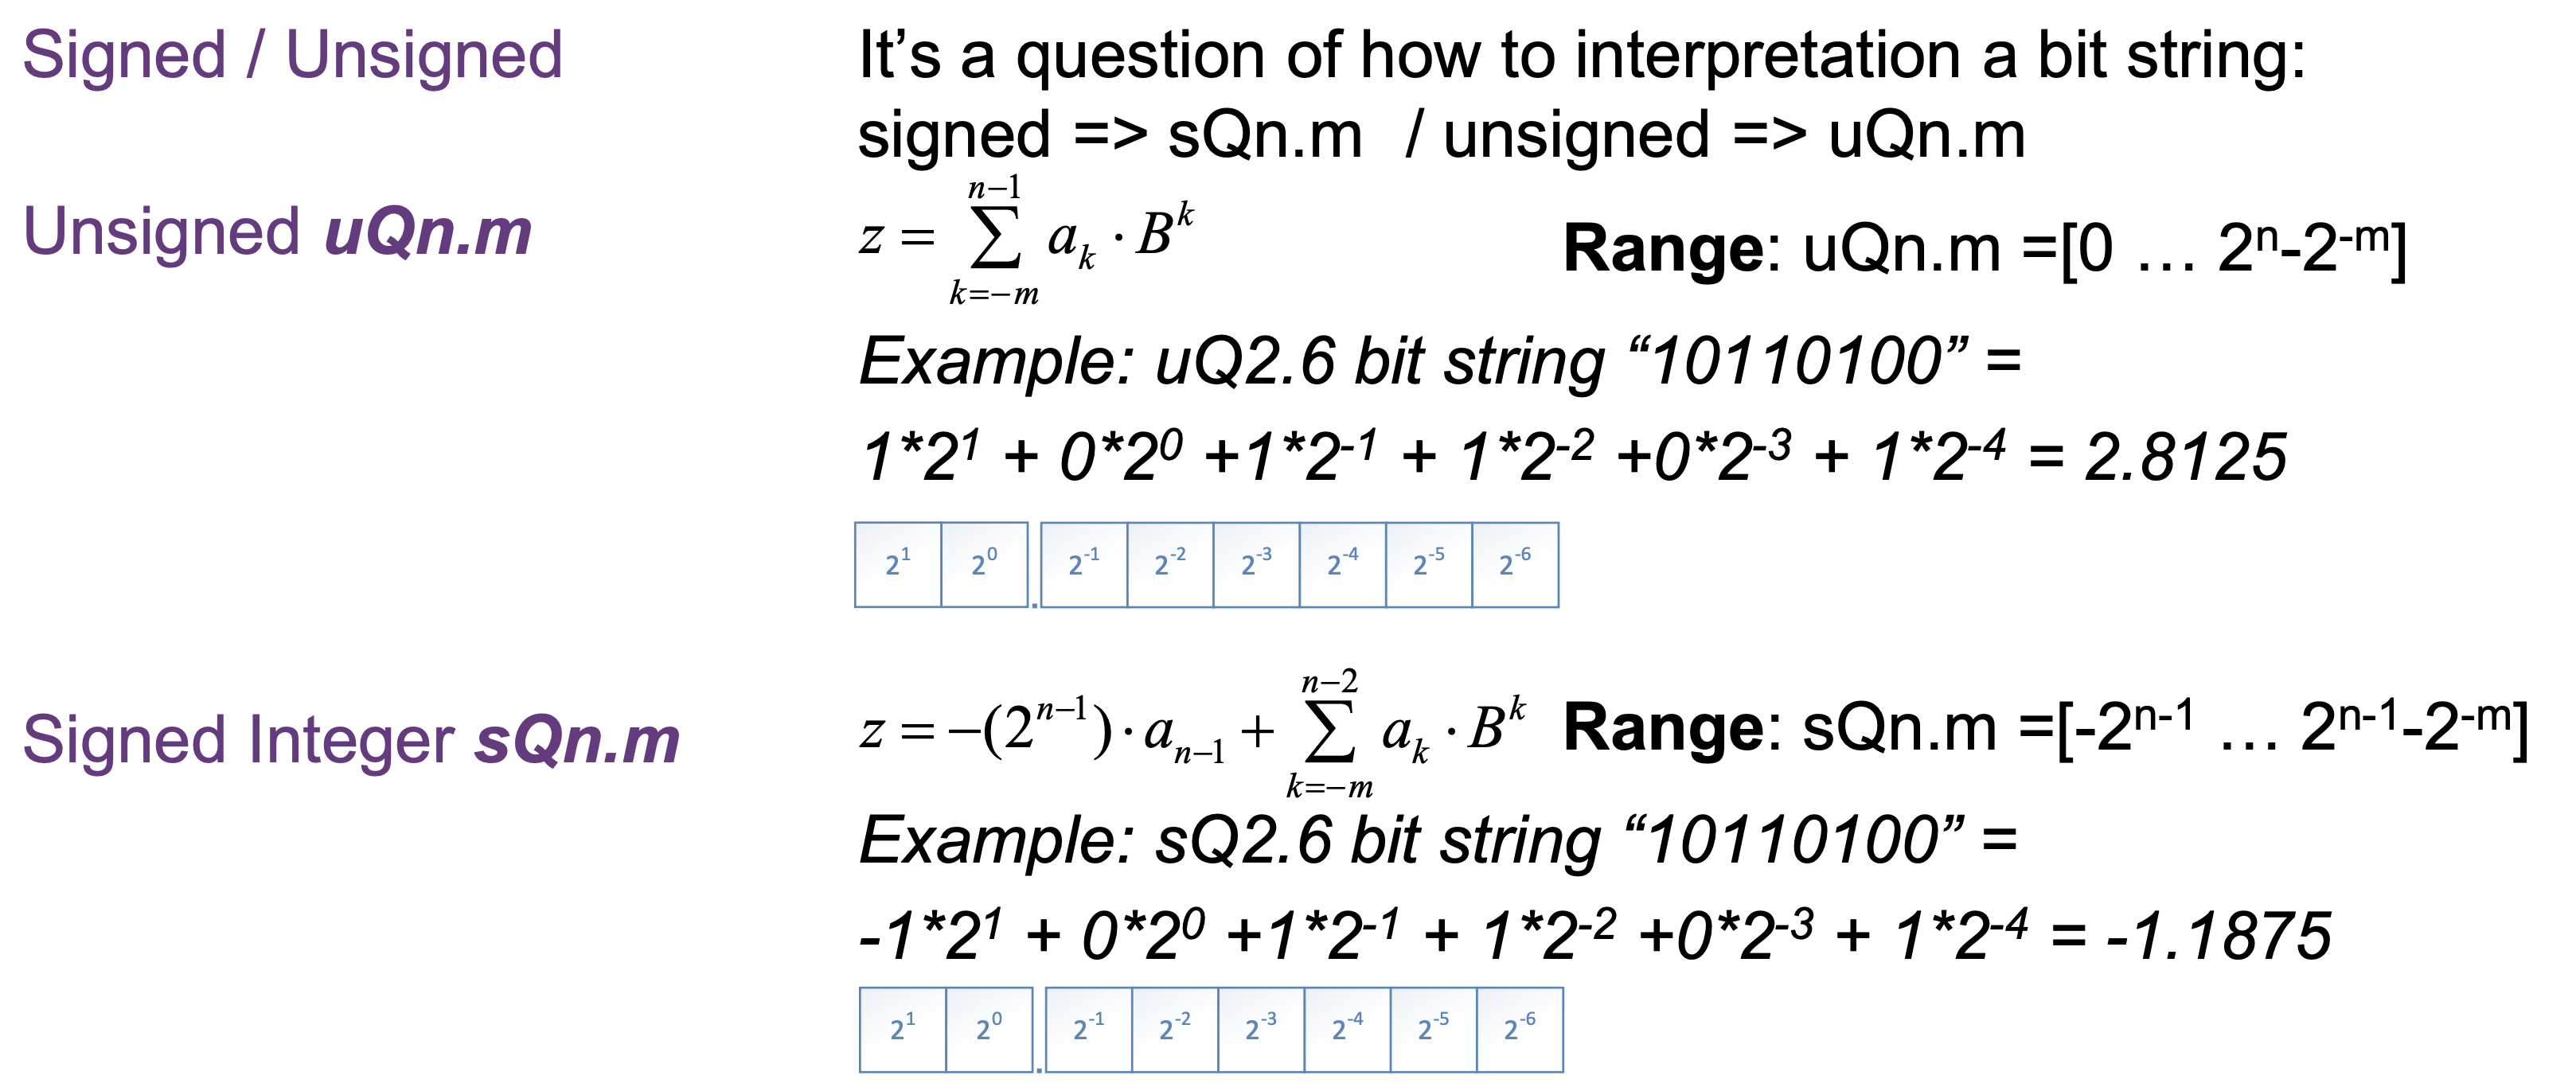
\includegraphics[width=\linewidth,height=0.24\textheight,keepaspectratio]{fig/L4_qnm_signed_unsigned.png}
  \caption{Qn.m-Darstellung: signed vs. unsigned, Wertebereich und Auflösung.}
\end{figure}

\subsection{Skalierung und Typkonvertierung}
Reale Zahlen werden durch Skalierung in Fixed Point überführt.

\subsubsection*{\textcolor{codeemph}{Prüfungsformeln}}
\[
\text{Fixed} = \lfloor \text{Real} \cdot 2^m \rfloor
\]
\[
\text{Real} = \text{Fixed} \cdot 2^{-m}
\]

\imp{Prüfungsregel:}  
Ohne \hilite{explizite} \hilite{Typkonvertierung} keine \hilite{Arithmetik} in VHDL.

\subsection{fixed\_pkg vs. klassische Umsetzung}
Die Bibliothek \texttt{fixed\_pkg} (VHDL-2008) bietet:
\begin{itemize}
  \item Automatisches Alignment
  \item Guard Bits
  \item Kontrollierte Rundung und Sättigung
\end{itemize}

\imp{Prüfungsfokus:}  
\hilite{Prüfungen} \hilite{verlangen} \hilite{meist} die klassische Umsetzung ohne \texttt{fixed\_pkg}.

\subsection{Addition und Subtraktion}

\subsubsection*{\textcolor{codeemph}{Formatregel (Prüfung)}}
\[
Q(n_1.m_1) + Q(n_2.m_2)
= Q(\max(n_1,n_2)+1).\max(m_1,m_2)
\]

Das zusätzliche Bit ist ein \textbf{Guard Bit}.

\subsubsection*{Vorgehen ohne fixed\_pkg}
\begin{enumerate}
  \item Fractional Bits angleichen
  \item Vorzeichenerweiterung
  \item Addition
  \item Optional: Abschneiden
\end{enumerate}

\begin{figure}[t]
  \centering
  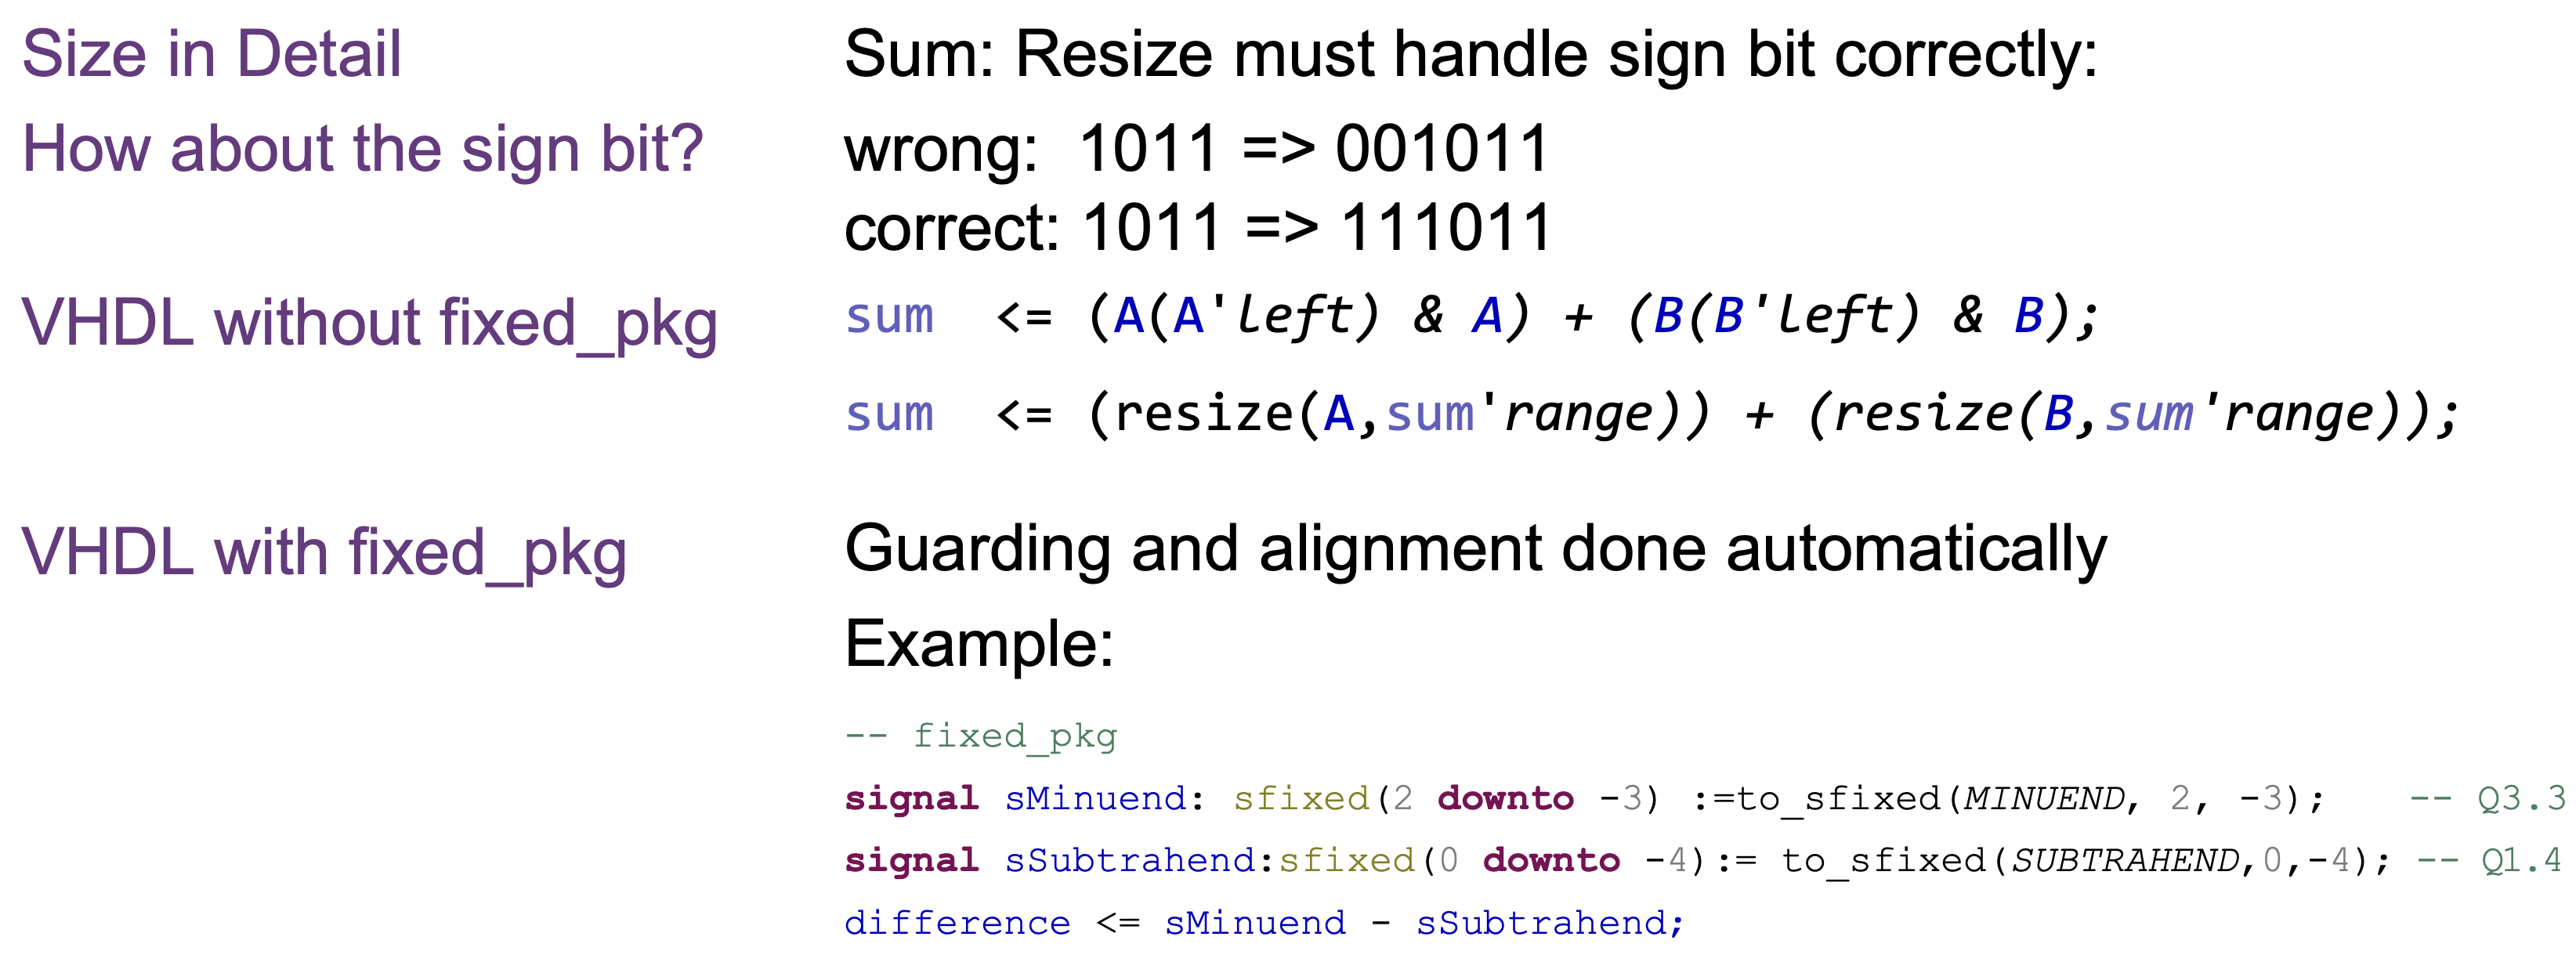
\includegraphics[width=\linewidth,height=0.24\textheight,keepaspectratio]{fig/L4_add_guardbit.png}
  \caption{Addition: Alignment und Guard Bit zur Überlaufabsicherung.}
\end{figure}

\subsubsection*{Additions-Code-Schablone}
\begin{lstlisting}[emph={entity,architecture,process,rising_edge,signal,constant,generic,port},emphstyle=\bfseries\color{codeemph}][emph={entity,architecture,process,rising_edge,signal,constant,generic,port},emphstyle=\bfseries\color{codeemph}]
A_ext <= signed(A) sll 1;
B_ext <= signed(B);
Y_ext <= A_ext + B_ext;
\end{lstlisting}

\imp{Prüfungsregel:}  
\hilite{Addition} \hilite{scheitert} meist an fehlendem \hilite{Guard Bit}.

\subsection{Multiplikation}

\subsubsection*{Formatregel}
\[
Q(n_1.m_1) \cdot Q(n_2.m_2)
= Q(n_1+n_2).(m_1+m_2)
\]

Bei signed $\times$ signed entsteht ein redundantes Vorzeichenbit:
\[
Q(n_1+n_2-1).(m_1+m_2)
\]

\begin{figure}[t]
  \centering
  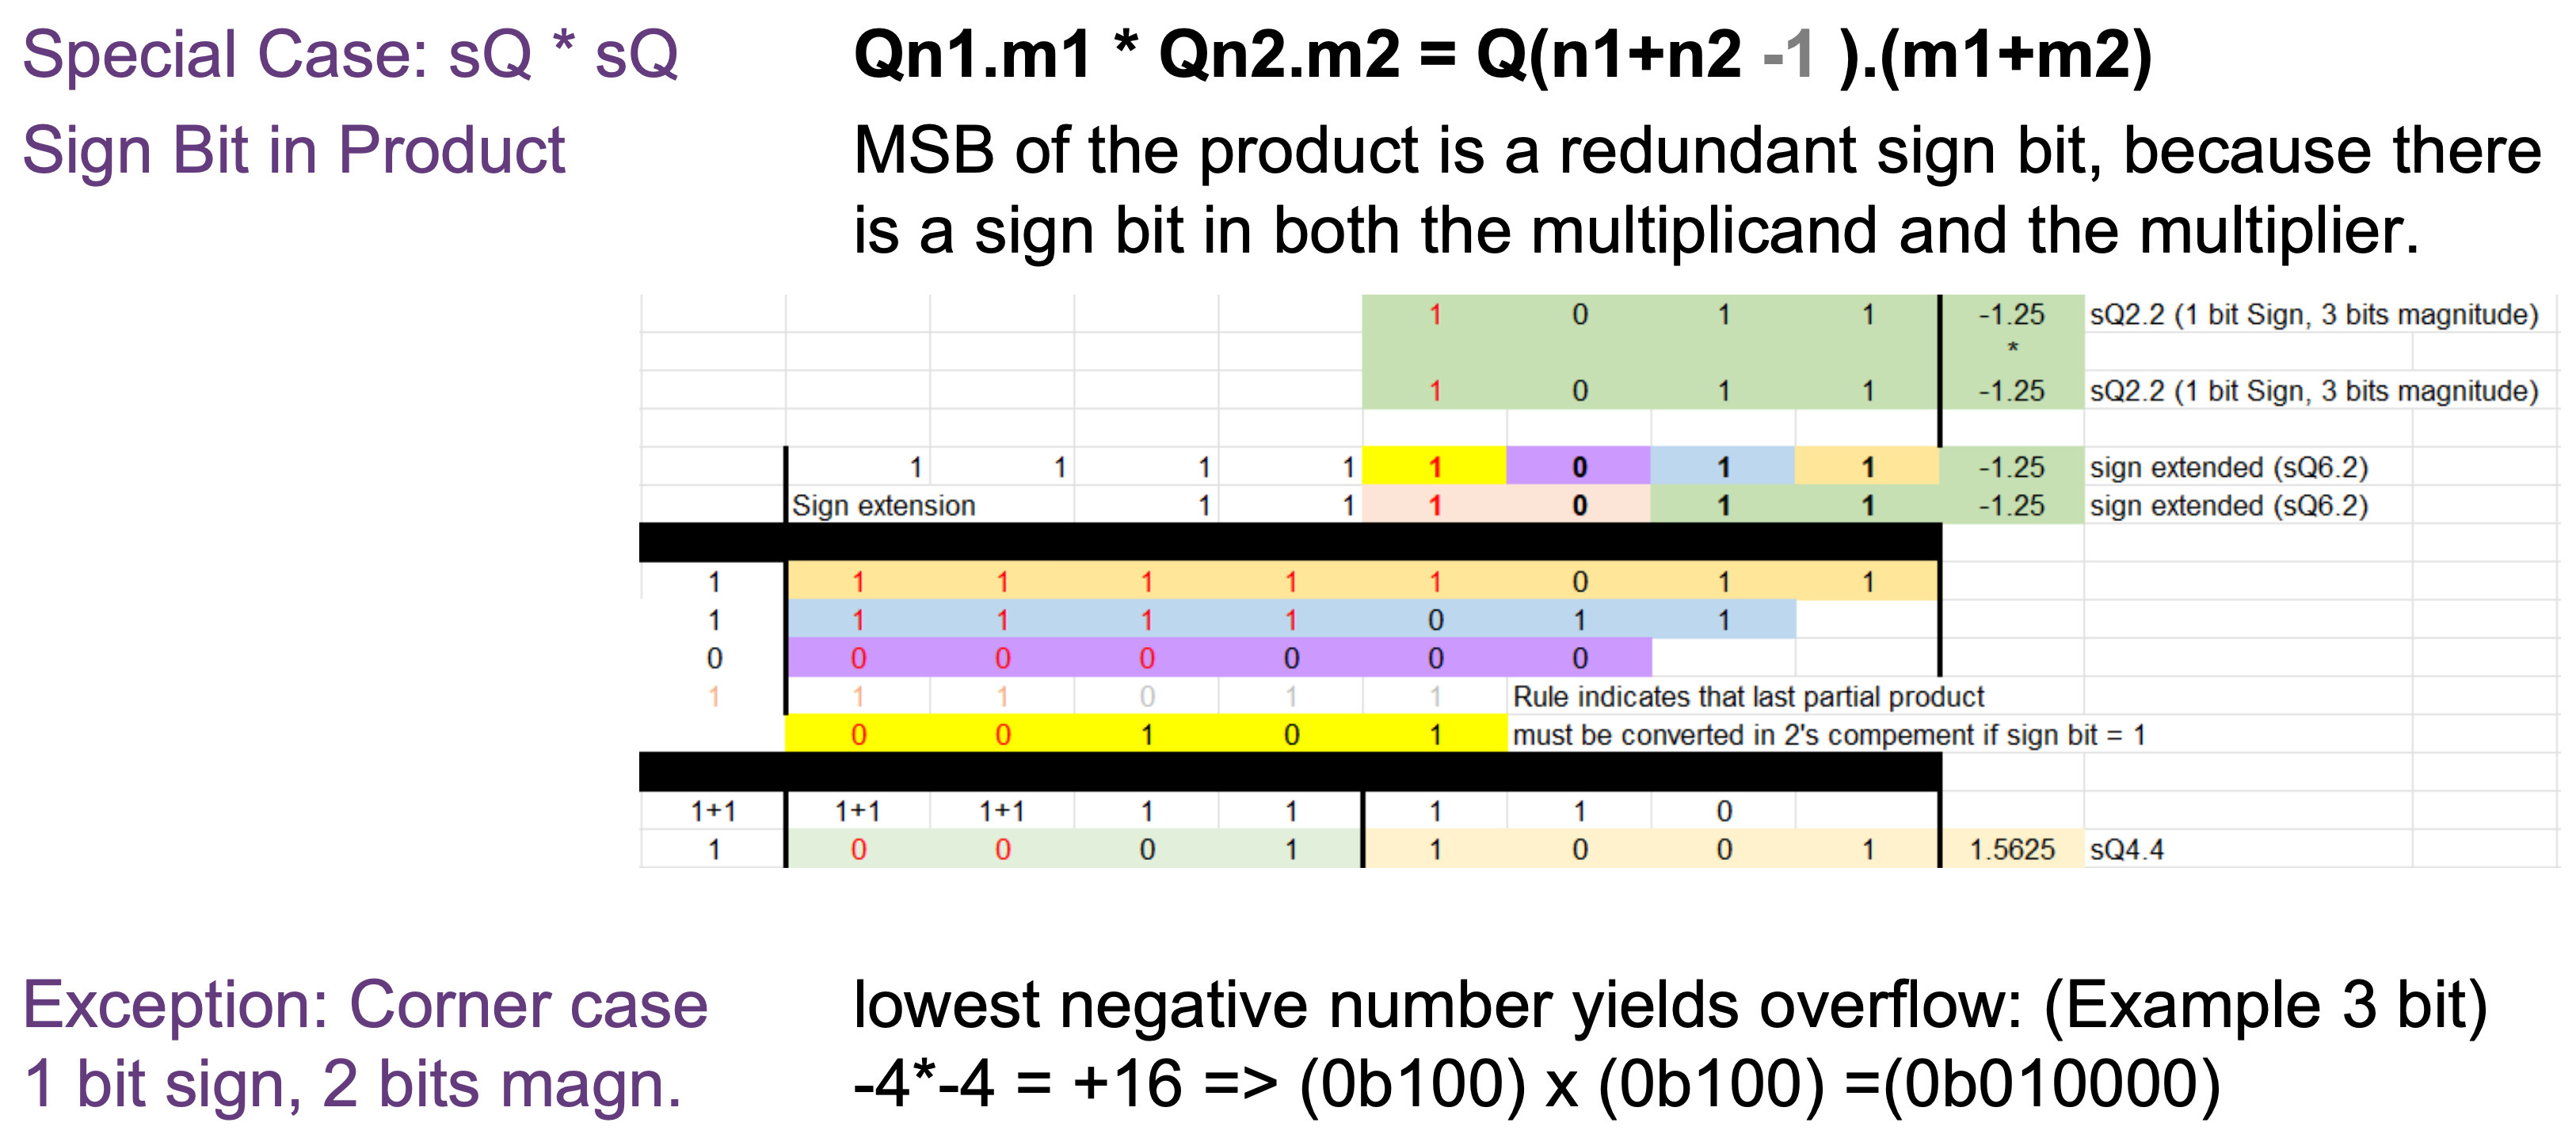
\includegraphics[width=\linewidth,height=0.22\textheight,keepaspectratio]{fig/L4_mult_redundant_sign.png}
  \caption{Multiplikation: resultierendes Format und redundantes Vorzeichenbit.}
\end{figure}

\subsubsection*{Multiplikations-Code-Schablone}
\begin{lstlisting}[emph={entity,architecture,process,rising_edge,signal,constant,generic,port},emphstyle=\bfseries\color{codeemph}]
P <= signed(A) * signed(B);
\end{lstlisting}

\imp{Prüfungsregel:}  
\hilite{Nach} der \hilite{Multiplikation} sind \hilite{fast} immer zu viele Bits vorhanden.

\subsection{Überlauf, Rundung und Sättigung}
Mögliche Effekte:
\begin{itemize}
  \item Wrap-Around (Überlauf)
  \item Sättigung
  \item Trunkierung
  \item Rundung
\end{itemize}

\imp{Prüfungsfokus:}  
\hilite{Trunkierung} und \hilite{Rundung} \hilite{unterscheiden} können.

\subsection{FIR-Filter als Anwendungsbeispiel}
Ein FIR-Filter besteht aus:
\begin{itemize}
  \item Verzögerungskette ($z^{-1}$)
  \item Multiplikationen
  \item Akkumulation
\end{itemize}

\textbf{Wortlängenstrategie (Prüfung):}
\begin{itemize}
  \item Produkt: redundantes Vorzeichenbit entfernen
  \item Zwischensumme: Guard Bits meist vernachlässigbar
  \item Endsumme: Guard Bit beibehalten
\end{itemize}

\begin{figure}[t]
  \centering
  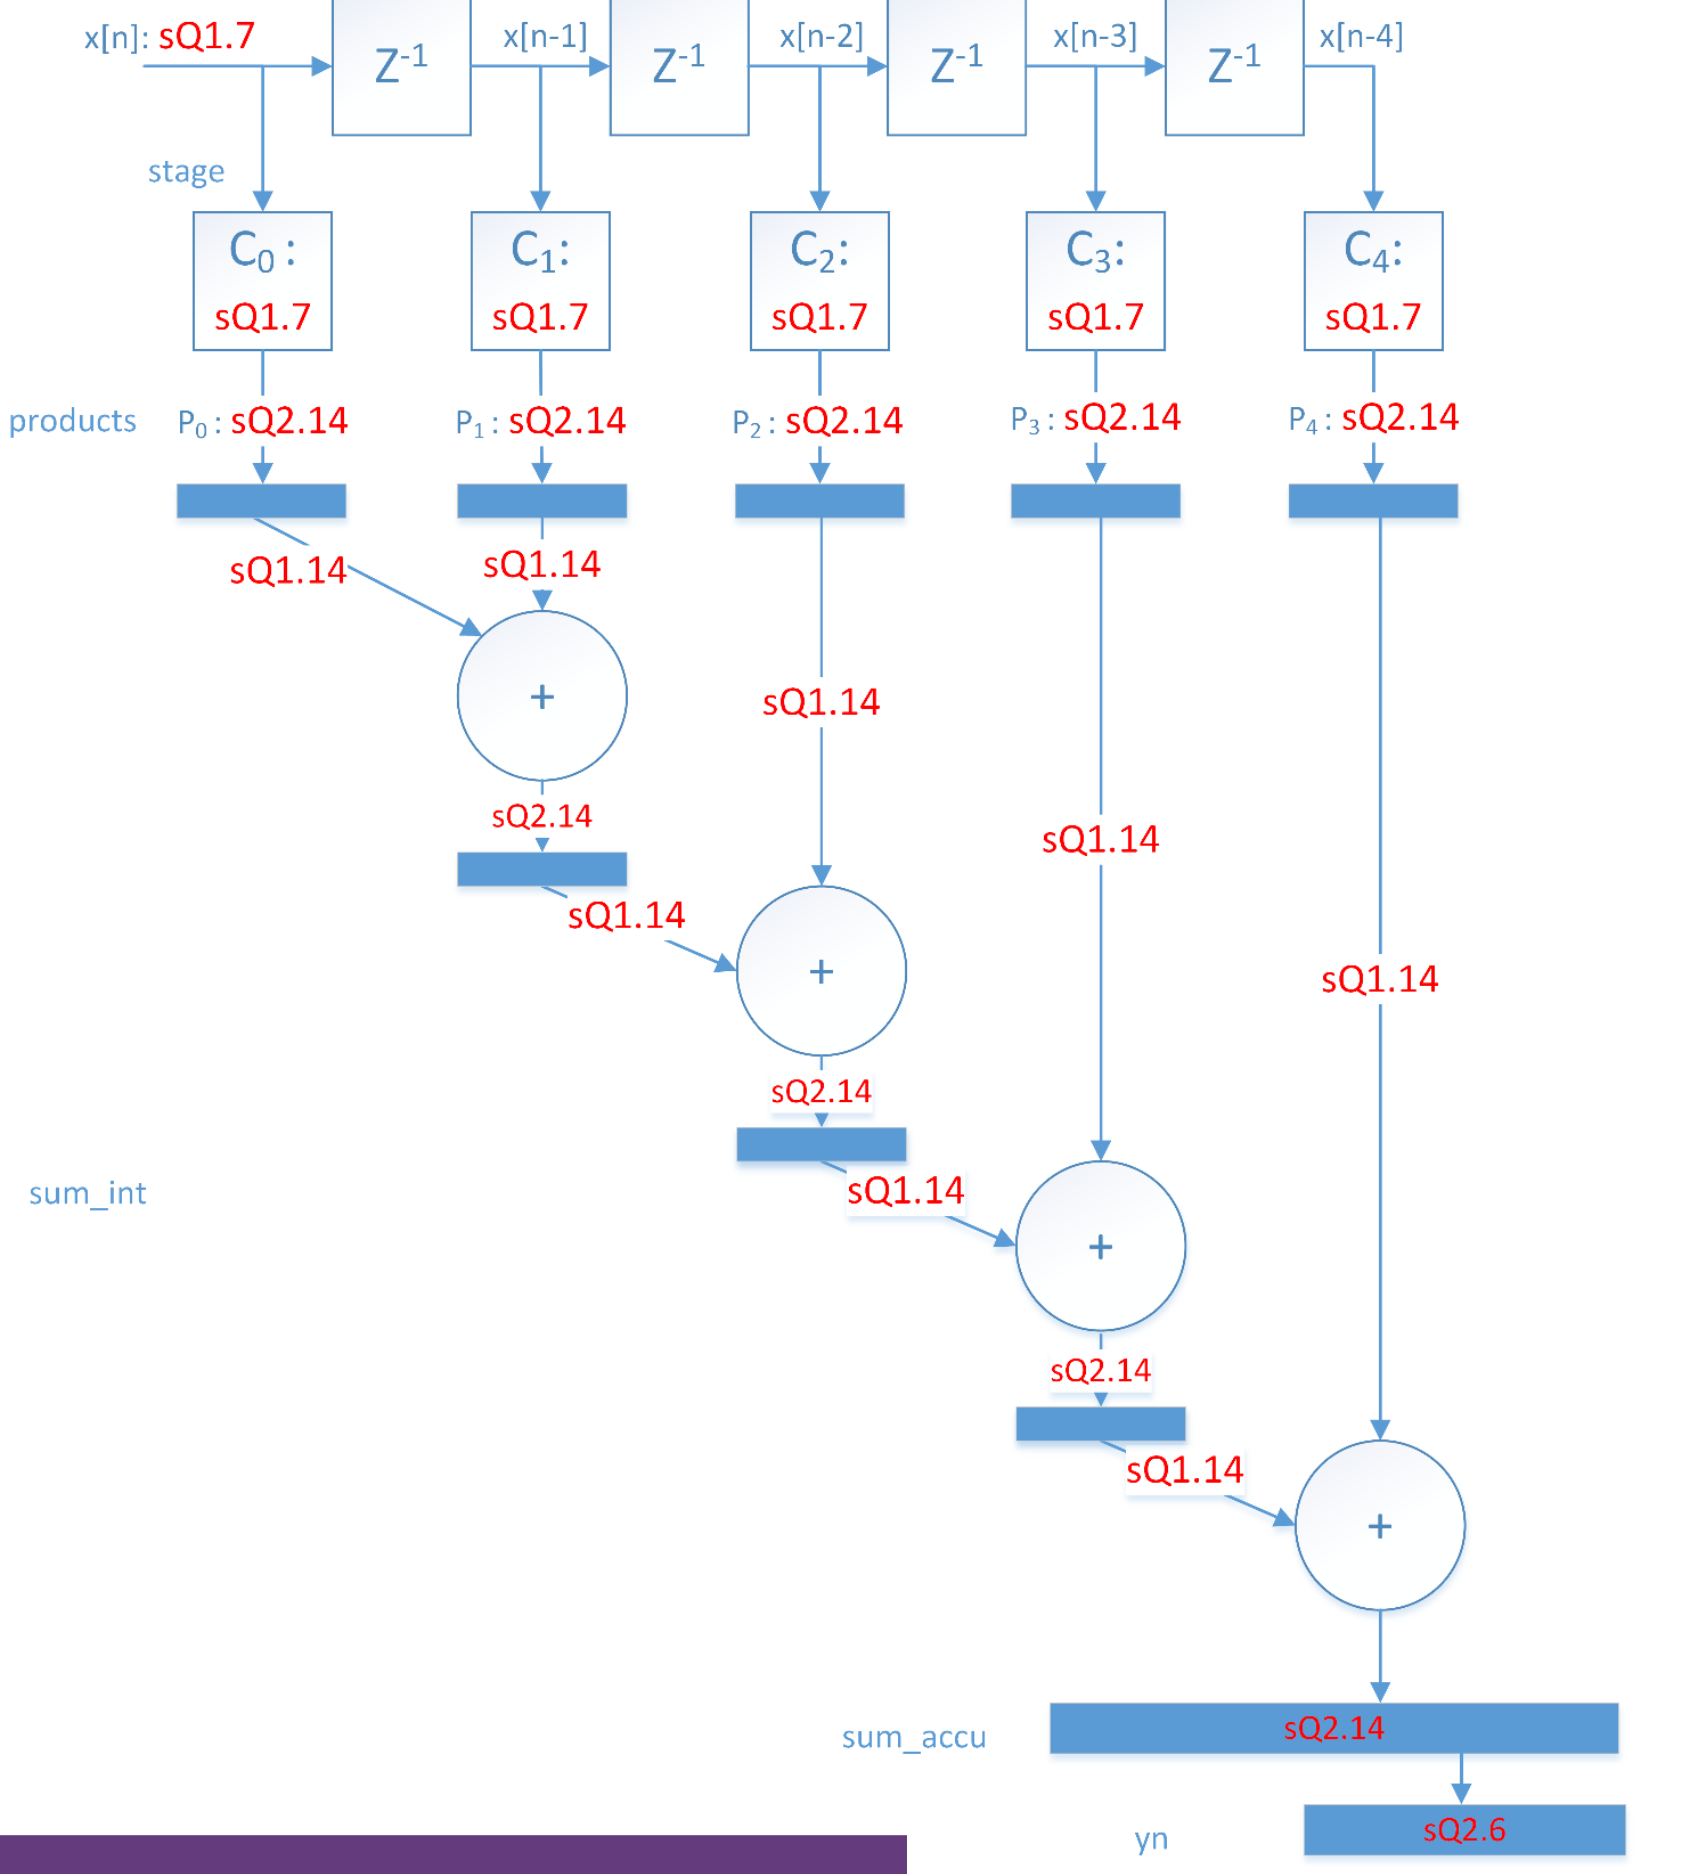
\includegraphics[width=\linewidth,height=0.26\textheight,keepaspectratio]{fig/L4_fir_qformats.png}
  \caption{FIR-Filter Blockdiagramm mit Q-Formaten für Produkte und Akkumulation.}
\end{figure}

\subsection{Systematische Wortlängenplanung}
Effiziente Fixed-Point-Systeme erfordern:
\begin{itemize}
  \item Analyse der Wertebereiche
  \item Konsistente Q-Formate
  \item Kontrollierte Guard Bits
\end{itemize}

\imp{Abschluss-Merksatz:}  
\hilite{Fixed Point} ist \hilite{kontrollierter} Fehler. Gute Planung schlägt hohe \hilite{Wortlänge}.


% ============================================================
\section{Custom IP Blocks: Memory}

\subsection{Einordnung und Ziel}
Speicher sind zentrale Bausteine digitaler Systeme und dominieren häufig Fläche, Energieverbrauch und Performance.  
Auf FPGAs existieren keine dedizierten ROM-Strukturen. RAM und ROM werden aus vorhandenen Hardware-Ressourcen abgebildet.

\imp{Merksatz (Prüfung):}  
\hilite{RAM} und \hilite{ROM} \hilite{unterscheiden} sich in VHDL primär durch das Zugriffsverhalten, nicht durch die Struktur.

Ziel ist die parametrisierbare Beschreibung, Initialisierung und Wiederverwendung von Speicherstrukturen als IP-Blöcke.

\subsection{Speichertypen}
Grundsätzlich wird zwischen RAM und ROM unterschieden:
\begin{itemize}
  \item \textbf{RAM}: Lesen und Schreiben zur Laufzeit
  \item \textbf{ROM}: Nur Lesen, konstante Inhalte
\end{itemize}

Technologisch:
\begin{itemize}
  \item \textbf{SRAM}: Statisch, kein Refresh
  \item \textbf{DRAM}: Dynamisch, Refresh erforderlich
\end{itemize}

FPGA-spezifisch:
\begin{itemize}
  \item \textbf{Distributed RAM} (LUT-basiert)
  \item \textbf{Block RAM} (dedizierte Hard-Macros)
\end{itemize}

\subsection{Speicherorganisation}
Logisch wird ein Speicher beschrieben durch:
\begin{itemize}
  \item \textbf{Breite}: Bits pro Wort
  \item \textbf{Tiefe}: Anzahl Wörter
\end{itemize}

\subsubsection*{\textcolor{codeemph}{Prüfungsformeln}}
\[
\text{Tiefe} = 2^{ADDR\_WIDTH}
\]
\[
\text{Gesamtbits} = \text{Breite} \cdot \text{Tiefe}
\]

\imp{Prüfungsregel:}  
\hilite{ADDR}\_\hilite{WIDTH} \hilite{bestimmt} die Anzahl Adressen, nicht die Wortbreite.

\subsection{Speicherports und Zugriffsarten}
Unterstützte Port-Typen:
\begin{itemize}
  \item \textbf{Single Port RAM}
  \item \textbf{Simple Dual Port RAM}
  \item \textbf{True Dual Port RAM}
\end{itemize}

\subsubsection*{\textcolor{codeemph}{Unterschiede (Prüfung)}}
\begin{itemize}
  \item Single Port: Lesen oder Schreiben
  \item Simple DP: ein Schreib-, ein Leseport
  \item True DP: zwei vollwertige Ports
\end{itemize}

\subsection{Zugriffsmodi bei Schreibkollisionen}
Bei gleichzeitigem Zugriff auf dieselbe Adresse:
\begin{itemize}
  \item \textbf{Write First}
  \item \textbf{Read First}
  \item \textbf{No Change}
\end{itemize}

\imp{Prüfungsregel:}  
Das \hilite{Verhalten} ist nicht \hilite{implizit}, \hilite{sondern} muss spezifiziert werden.

\subsection{Distributed RAM}
Distributed RAM nutzt LUTs (SLICEMs):
\begin{itemize}
  \item Schreiben synchron
  \item Lesen asynchron
  \item Kleine, schnelle Speicher
\end{itemize}

\imp{Prüfungsregel:}  
A\hilite{synchron}es \hilite{Lesen} $\rightarrow$ \hilite{Distributed RAM}.

\subsection{Block RAM}
Block RAM besteht aus dedizierten Hard-Macros:
\begin{itemize}
  \item 36\,kb physisch, ca. 32\,kb nutzbar
  \item Synchrones Lesen und Schreiben
  \item Unterstützt ECC und FIFO
\end{itemize}

\imp{Prüfungsregel:}  
\hilite{Synchrones} \hilite{Lesen} $\rightarrow$ \hilite{Block RAM}.

\begin{figure}[t]
  \centering
  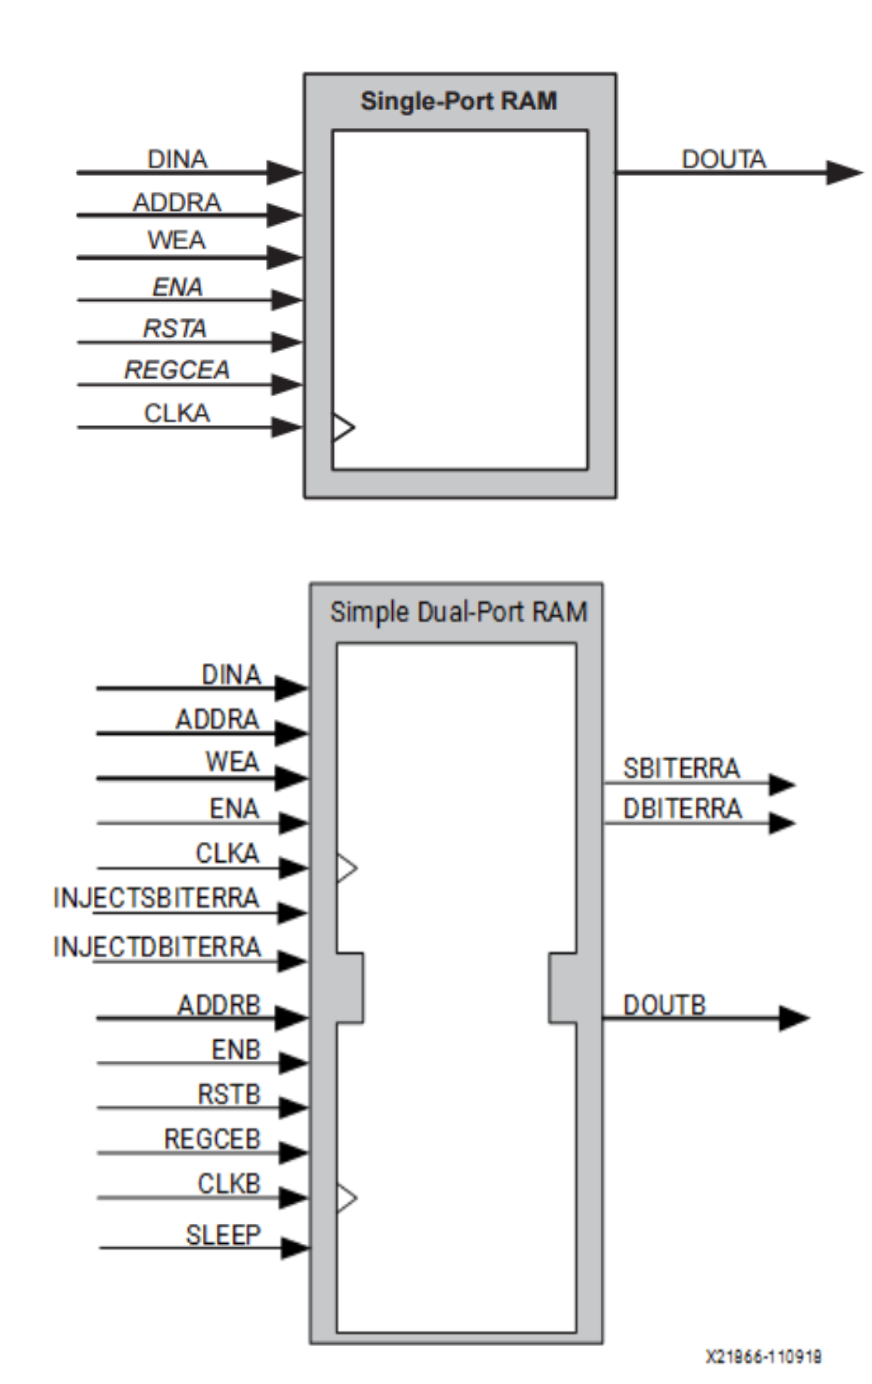
\includegraphics[width=\linewidth,height=0.26\textheight,keepaspectratio]{fig/L5_ram_overview.png}
  \caption{RAM-Organisation und Implementierung als Block RAM oder Distributed RAM.}
\end{figure}

\subsection{VHDL-Modellierung von RAM}

\subsubsection*{Grundregeln}
\begin{itemize}
  \item Breite und Tiefe über Generics
  \item Eindimensionales Array
  \item Ein Prozess pro Port
\end{itemize}

\subsubsection*{Single Port RAM – Code-Schablone}
\begin{lstlisting}[emph={entity,architecture,process,rising_edge,signal,constant,generic,port},emphstyle=\bfseries\color{codeemph}][emph={entity,architecture,process,rising_edge,signal,constant,generic,port},emphstyle=\bfseries\color{codeemph}]
type ram_t is array (0 to DEPTH-1) of std_logic_vector(W-1 downto 0);
signal ram : ram_t;

process(clk)
begin
  if rising_edge(clk) then
    if we='1' then
      ram(addr) <= din;
    end if;
    dout <= ram(addr);
  end if;
end process;
\end{lstlisting}

\subsubsection*{True Dual Port RAM – Hinweis}
True Dual Port RAM wird häufig besser über dedizierte Block-RAM-IP realisiert.  
Eine VHDL-Modellierung mit \texttt{shared variable} ist simulatorfreundlich, aber kritisch.

\subsection{Synthesis-Attribute}
Die Implementierung kann gezielt beeinflusst werden:

\begin{lstlisting}[emph={entity,architecture,process,rising_edge,signal,constant,generic,port},emphstyle=\bfseries\color{codeemph}][emph={entity,architecture,process,rising_edge,signal,constant,generic,port},emphstyle=\bfseries\color{codeemph}]
attribute ram_style : string;
attribute ram_style of ram : signal is "block";
\end{lstlisting}

Alternativ:
\begin{lstlisting}[emph={entity,architecture,process,rising_edge,signal,constant,generic,port},emphstyle=\bfseries\color{codeemph}][emph={entity,architecture,process,rising_edge,signal,constant,generic,port},emphstyle=\bfseries\color{codeemph}]
attribute ram_style of ram : signal is "distributed";
\end{lstlisting}

\imp{Merksatz (Prüfung):}  
\hilite{Attribute} sind \hilite{Hinweise} an das \hilite{Tool}, keine funktionalen Anweisungen.

\subsection{ROM-Implementierung}
ROM unterscheidet sich von RAM nur durch konstante Inhalte.

\subsubsection*{ROM – Code-Schablone}
\begin{lstlisting}[emph={entity,architecture,process,rising_edge,signal,constant,generic,port},emphstyle=\bfseries\color{codeemph}][emph={entity,architecture,process,rising_edge,signal,constant,generic,port},emphstyle=\bfseries\color{codeemph}]
type rom_t is array (0 to 15) of std_logic_vector(7 downto 0);
constant rom : rom_t := (
  0 => x"12",
  1 => x"34",
  others => x"00"
);
\end{lstlisting}

\subsection{Speicherinitialisierung}
Möglichkeiten:
\begin{itemize}
  \item Initialisierung bei Deklaration
  \item Datei-basierte Initialisierung (.coe, .mif)
\end{itemize}

\imp{Prüfungsregel:}  
\hilite{ROM} ohne \hilite{Initialisierung} ist \hilite{inhaltlich} wertlos.

\subsection{Memory Generator IP}
Xilinx stellt parametrische Speicher-IP bereit:
\begin{itemize}
  \item Frei wählbare Breite und Tiefe
  \item Konfigurierbare Zugriffsmodi
  \item Native oder AXI4-Schnittstelle
\end{itemize}

\subsection{IP-Wiederverwendung und Integration}
IP-Blöcke sind parametrisierte, wiederverwendbare Einheiten.

\begin{itemize}
  \item Hard IP
  \item Firm IP
  \item Soft IP
\end{itemize}

Integration:
\begin{itemize}
  \item IP Integrator
  \item RTL-Instantiation
\end{itemize}

\begin{figure}[t]
  \centering
  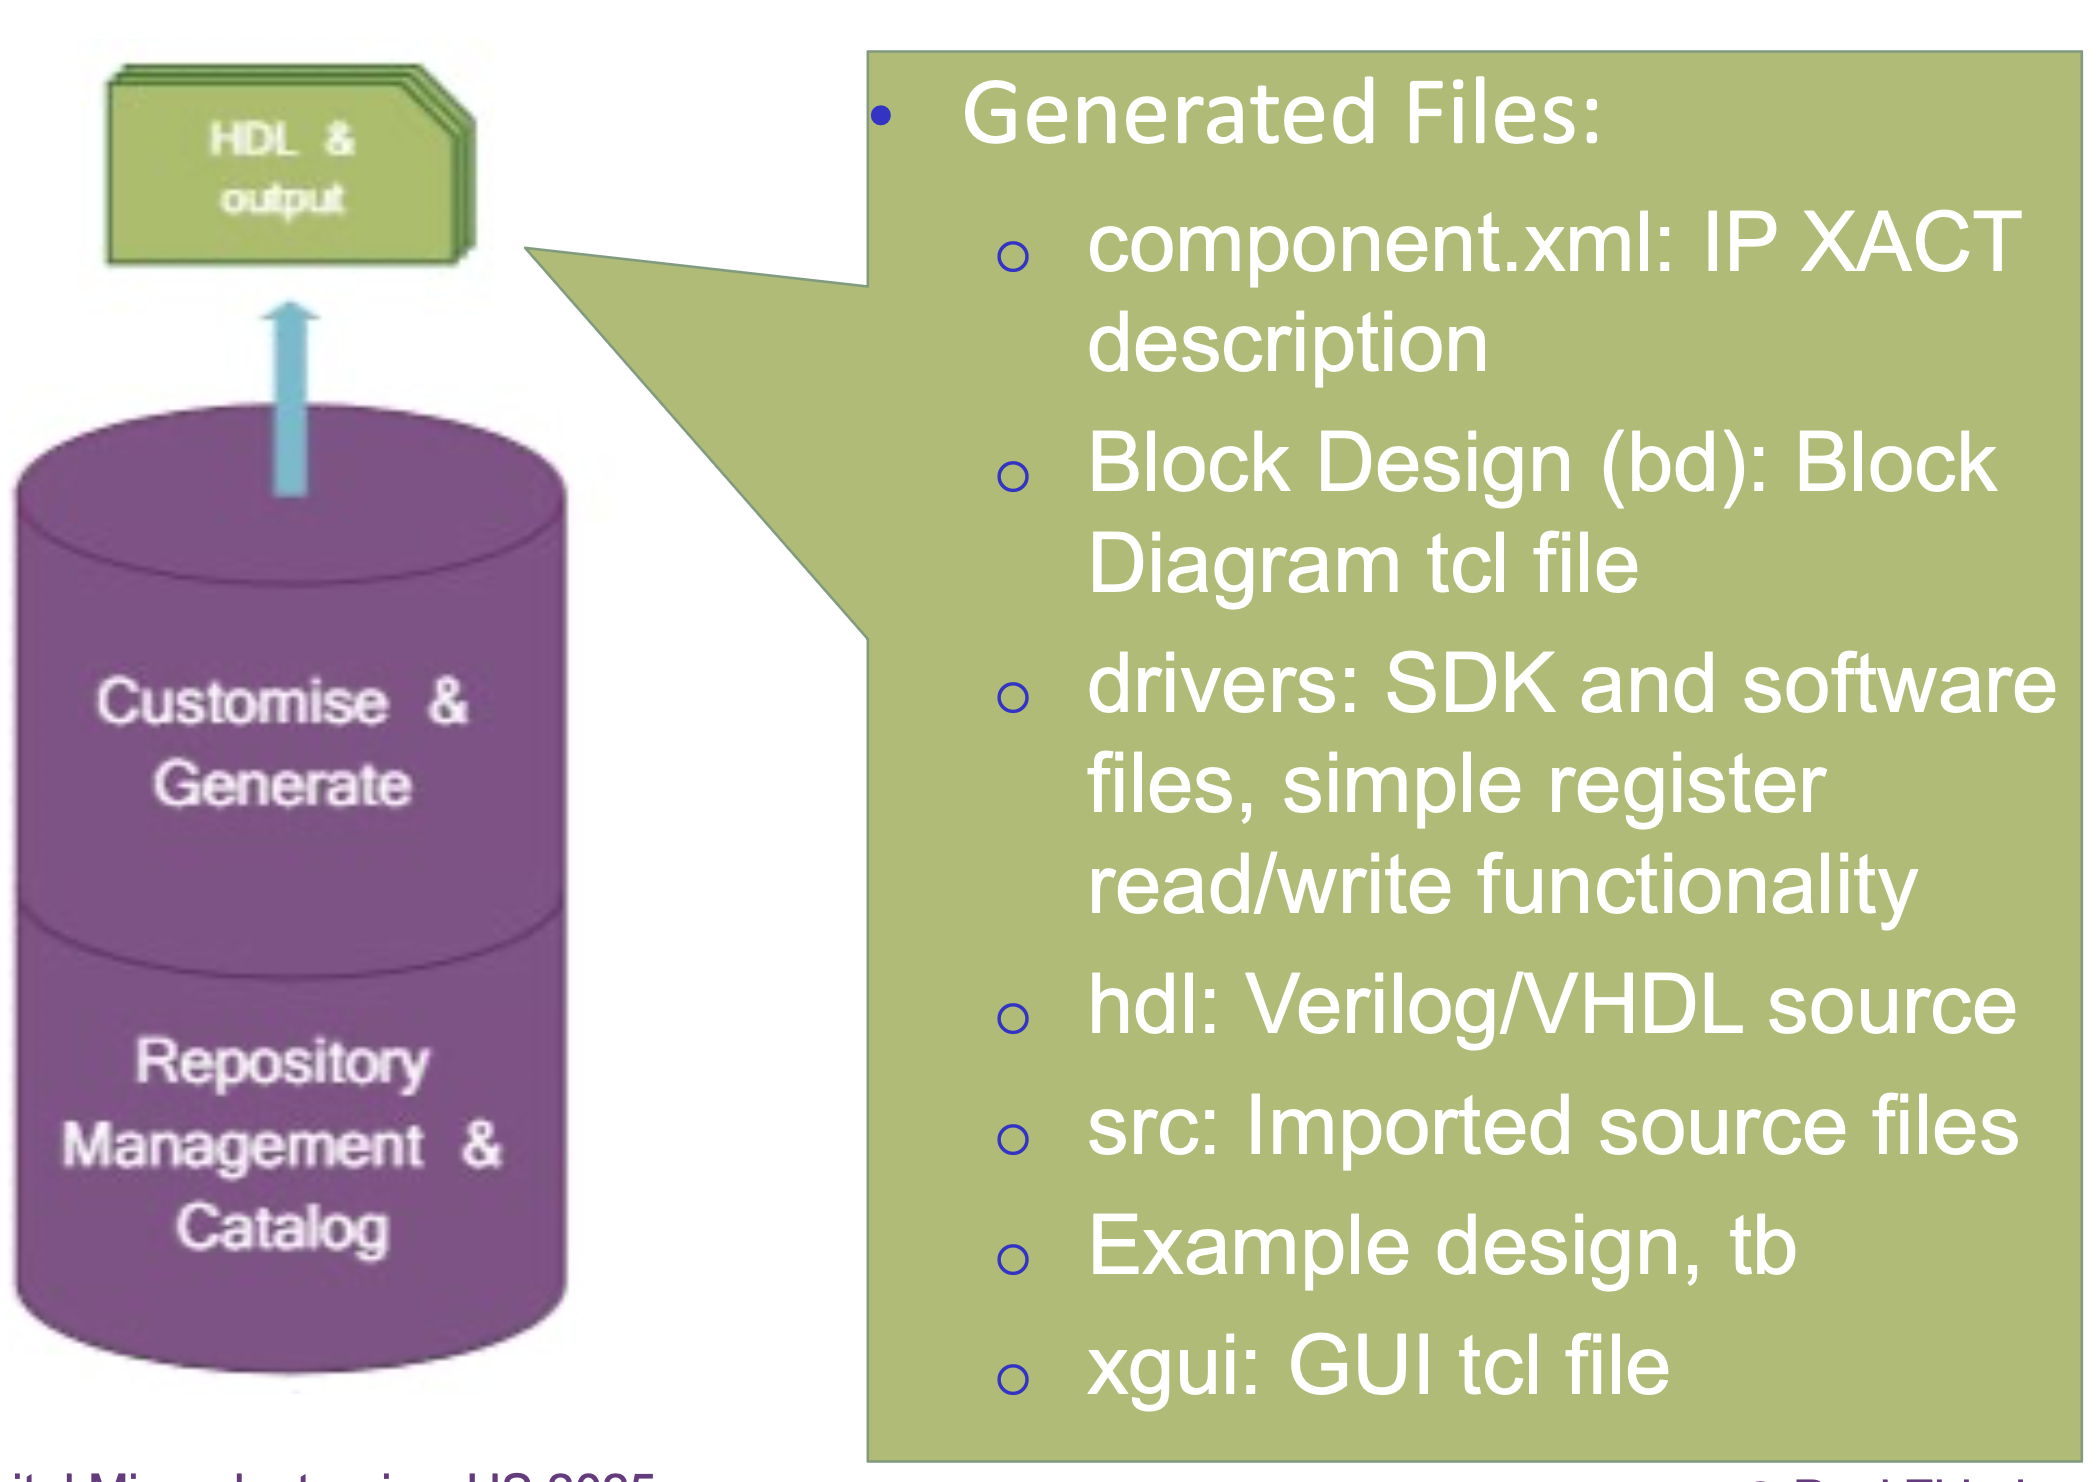
\includegraphics[width=\linewidth,height=0.26\textheight,keepaspectratio]{fig/L5_design_workflow.png}
  \caption{ARM-Prototyp und Design-Workflow im IP Integrator.}
\end{figure}

\subsection{IP Lifecycle}
IP-Blöcke unterliegen Versions- und Lebenszyklen:
\begin{itemize}
  \item Pre-Production
  \item Production
  \item Superseded
  \item Discontinued
\end{itemize}

\imp{Abschluss-Merksatz:}  
\hilite{Gute} Speicher-\hilite{IP} ist parametrisch, \hilite{synchron} und eindeutig spezifiziert.



% ============================================================
\section{Serial Communication Interfaces}

\subsection{Systematische Einordnung}
Serielle Kommunikationsschnittstellen verbinden digitale Systeme auf Chip-, Board- oder Systemebene.  
Sie lassen sich entlang mehrerer Dimensionen klassifizieren:
\begin{itemize}
  \item \textbf{Topologie:} Point-to-Point, Bus, Stern, Daisy-Chain
  \item \textbf{Datenorganisation:} Seriell vs. Parallel
  \item \textbf{Zeitorganisation:} Synchron vs. Asynchron
  \item \textbf{Physikalische Umsetzung:} Single-Ended vs. Differenziell
\end{itemize}

\imp{Prüfungsregel:}  
\hilite{Serielle} \hilite{Kommunikation} spart \hilite{Pins}, erhöht aber die Logikkomplexität.

Die Vorlesung behandelt ausschließlich Physical Layer und Data Link Layer.

\begin{figure}[t]
  \centering
  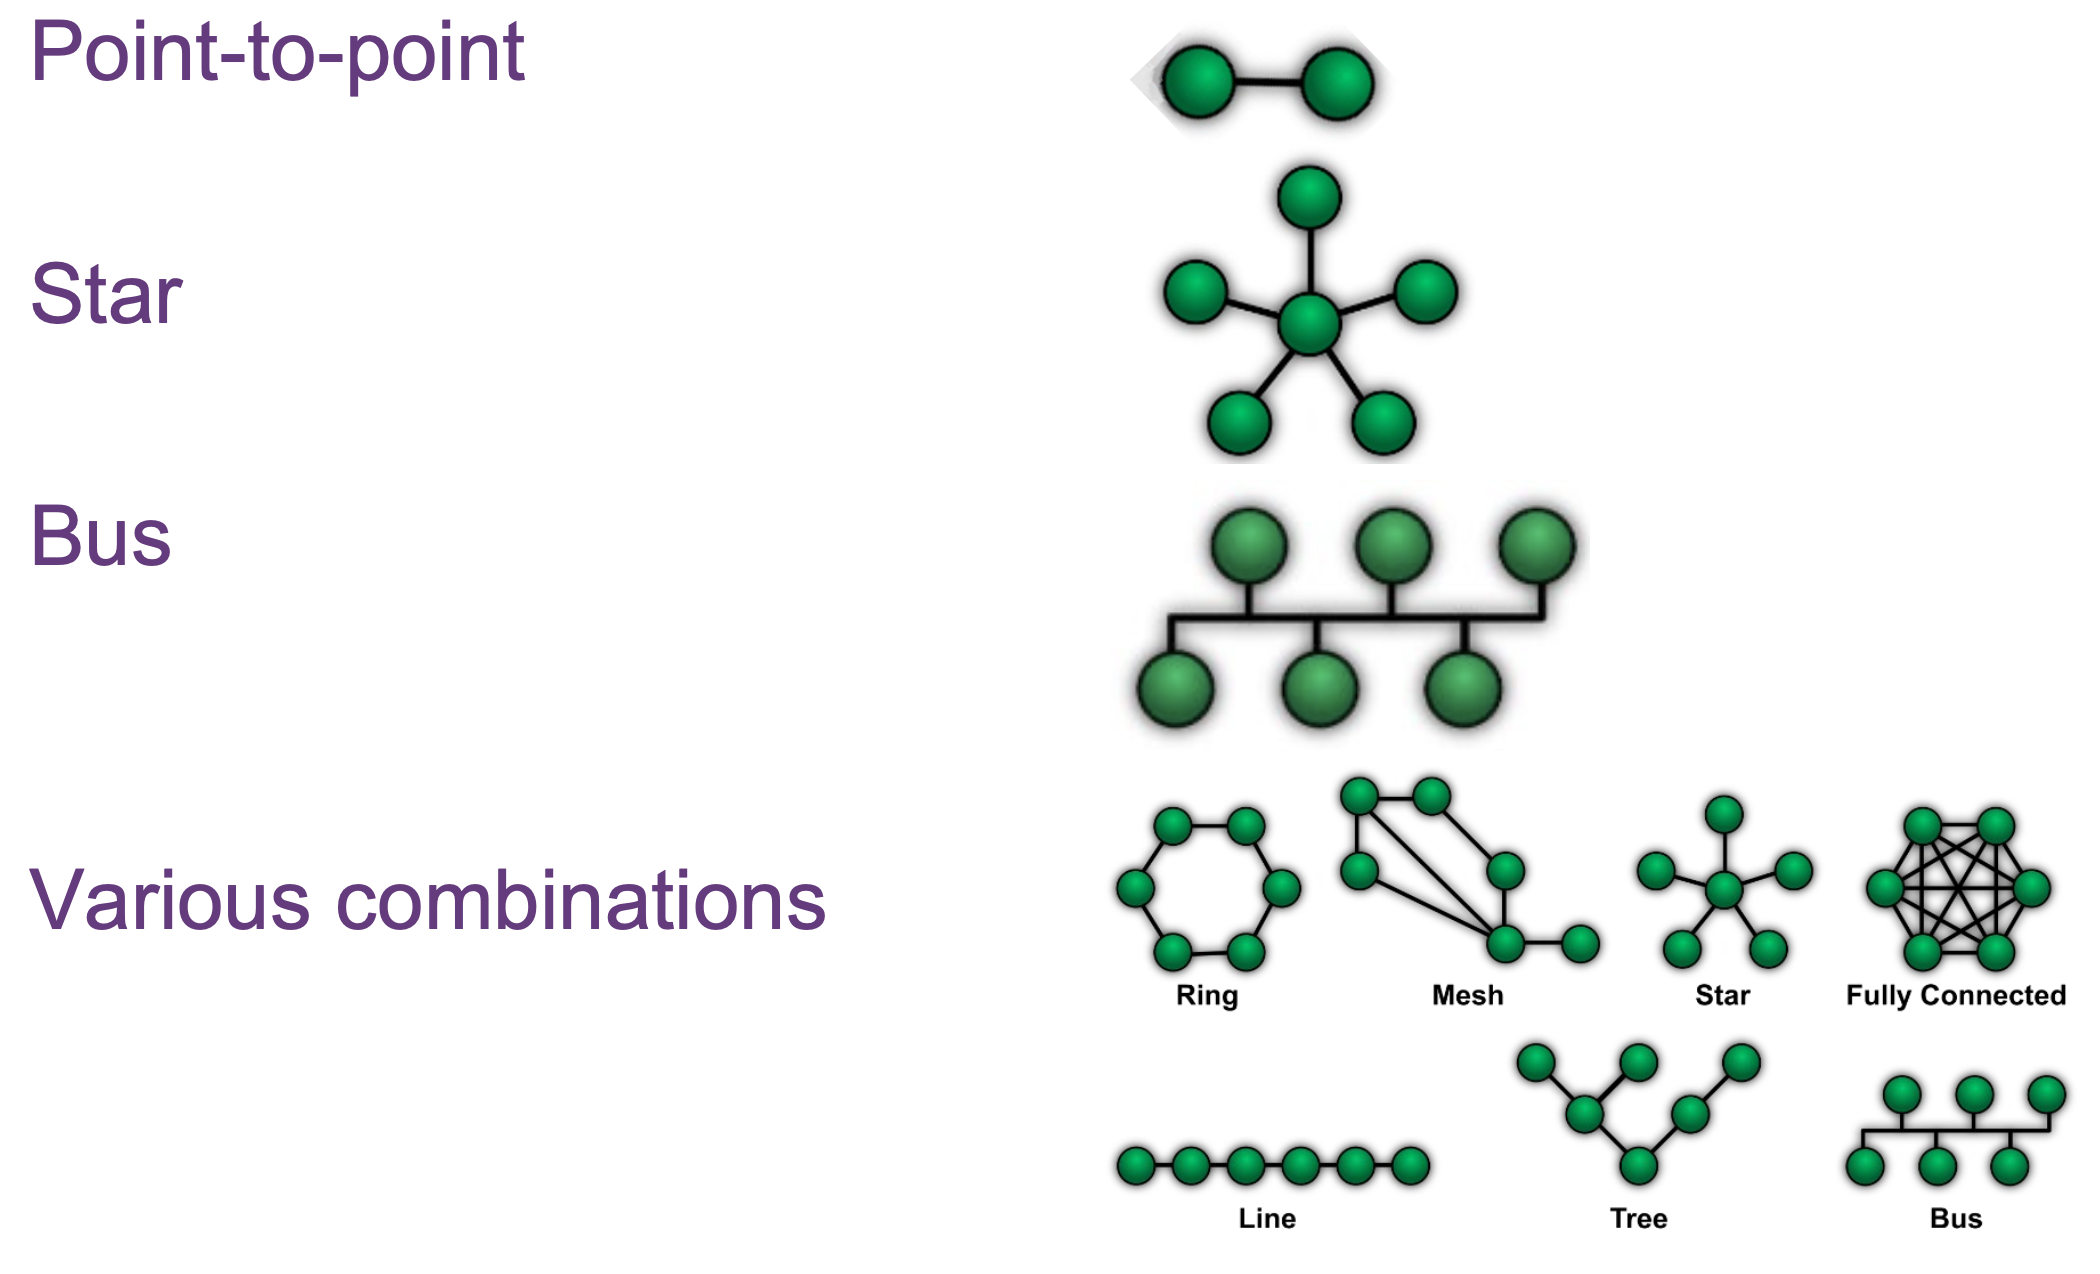
\includegraphics[width=\linewidth,height=0.24\textheight,keepaspectratio]{fig/L6_classification_serial.png}
  \caption{Klassifikation serieller Schnittstellen nach Topologie und Datenorganisation.}
\end{figure}

\subsection{Logik-zu-Physik-Übersetzung}
VHDL-Signale sind rein logisch und müssen über I/O-Pads physikalisch umgesetzt werden.

Relevante Parameter:
\begin{itemize}
  \item I/O-Standard
  \item Single-Ended oder differentiell
  \item Slew Rate und Drive Strength
  \item Pull-Up, Pull-Down, Keeper
\end{itemize}

\imp{Merksatz (Prüfung):}  
\hilite{Pads} \hilite{bestimmen} das \hilite{elektrische} Verhalten, nicht das Protokoll.

\subsection{Spannungs- und Strommodus}

\textbf{Voltage Mode:}
\begin{itemize}
  \item Logik über Spannungspegel
  \item Einfach, aber hoher Energieverbrauch
\end{itemize}

\textbf{Current Mode:}
\begin{itemize}
  \item Logik über Stromrichtung
  \item Kleiner Spannungs-Hub
  \item Besser für hohe Datenraten
\end{itemize}

\imp{Prüfungsregel:}  
\hilite{Hohe} \hilite{Datenrate} $\rightarrow$ \hilite{Current Mode}.

\subsection{LVDS}
LVDS ist eine differentielle Strommodus-Signalisierung.

Kenndaten:
\begin{itemize}
  \item Strom: $\pm 3.5$\,mA
  \item Terminierung: $\approx 100\,\Omega$
  \item Signalhub: $\approx \pm 350$\,mV
\end{itemize}

Vorteile:
\begin{itemize}
  \item Hohe Geschwindigkeit
  \item Geringe EMV
  \item Hohe Störfestigkeit
\end{itemize}

LVDS wird über Constraints konfiguriert und nutzt spezielle Buffer.

\begin{figure}[t]
  \centering
  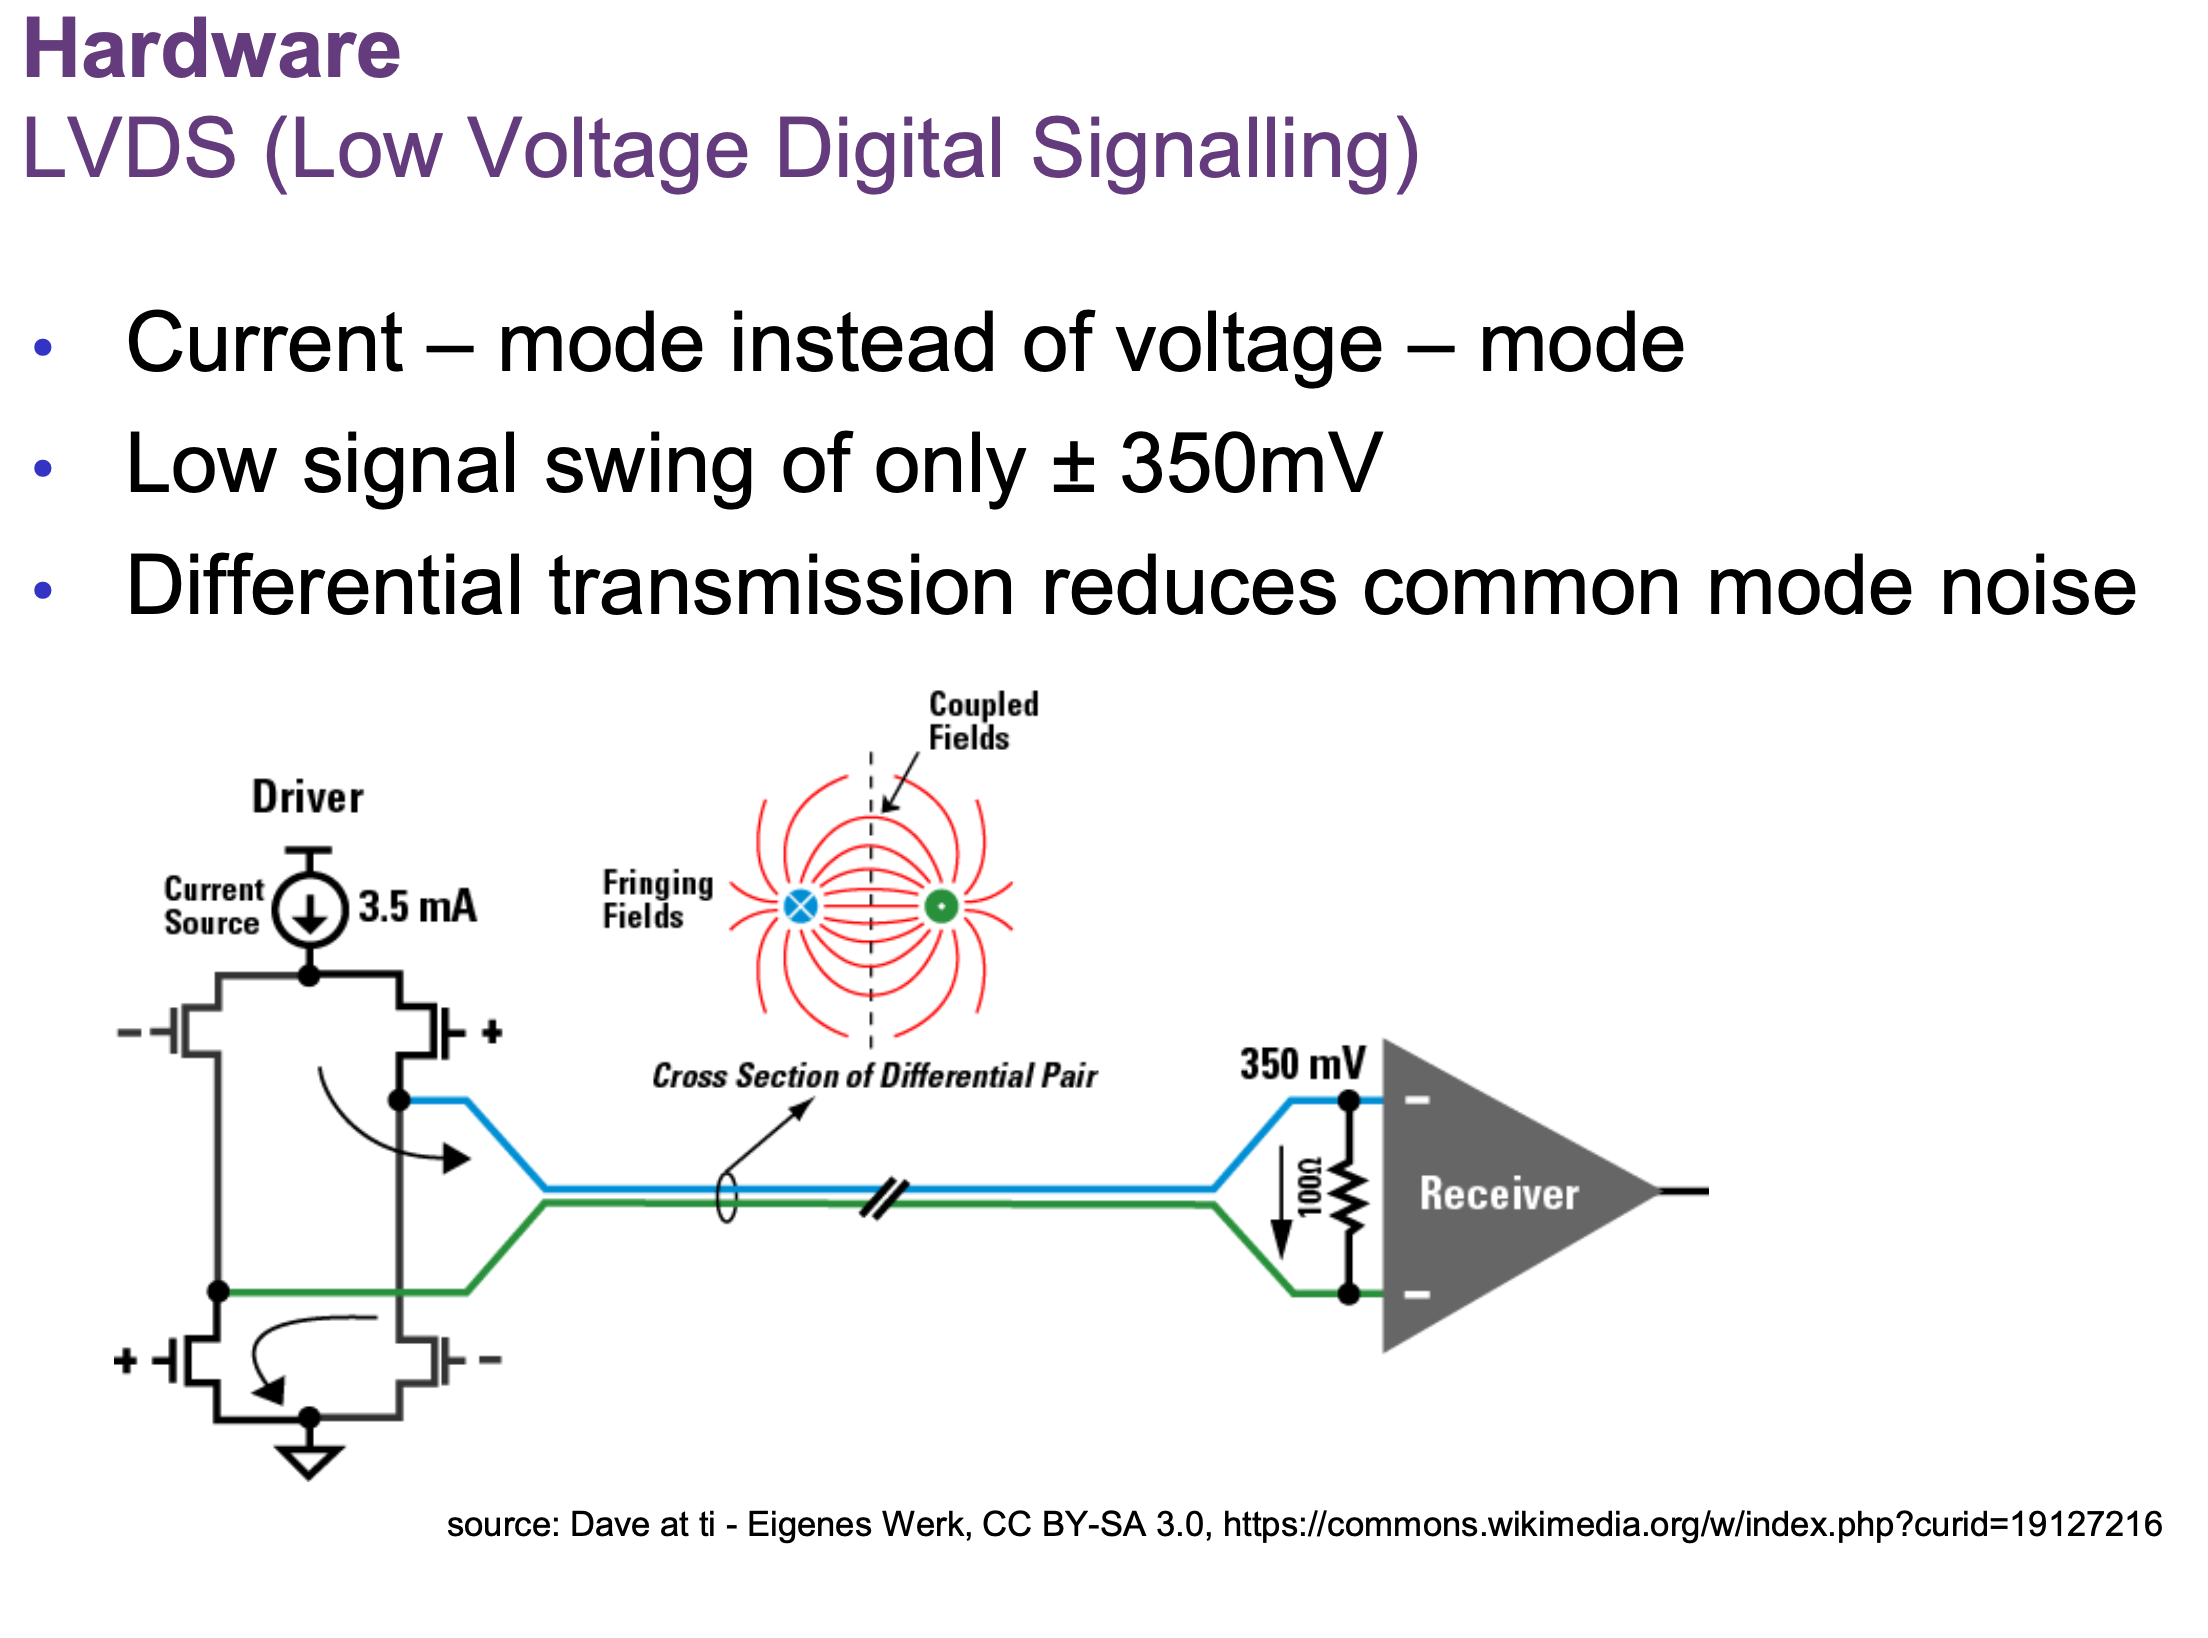
\includegraphics[width=\linewidth,height=0.24\textheight,keepaspectratio]{fig/L6_lvds_pad.png}
  \caption{LVDS-Prinzip und Umsetzung über FPGA-I/O-Pads.}
\end{figure}

\subsection{Serialisierung und Deserialisierung}
Serielle Schnittstellen benötigen SERDES-Strukturen:
\begin{itemize}
  \item Parallel-In / Serial-Out (PISO)
  \item Serial-In / Parallel-Out (SIPO)
\end{itemize}

Grundbaustein ist ein Schieberegister mit FSM-Steuerung.

\subsubsection*{Schieberegister – Code-Schablone}
\begin{lstlisting}[emph={entity,architecture,process,rising_edge,signal,constant,generic,port},emphstyle=\bfseries\color{codeemph}][emph={entity,architecture,process,rising_edge,signal,constant,generic,port},emphstyle=\bfseries\color{codeemph}]
if rising_edge(clk) then
  if load='1' then
    shreg <= data_in;
  elsif shift='1' then
    shreg <= shreg(W-2 downto 0) & '0';
  end if;
end if;
\end{lstlisting}

\subsection{SPI – Serial Peripheral Interface}
SPI ist eine synchrone, serielle Punkt-zu-Punkt-Schnittstelle.

Signale:
\begin{itemize}
  \item CS, SCLK, MOSI, MISO
\end{itemize}

Eigenschaften:
\begin{itemize}
  \item Master-Slave
  \item Vollduplex
\end{itemize}

Übertragungsparameter:
\begin{itemize}
  \item Clock Polarity (CPOL)
  \item Clock Phase (CPHA)
\end{itemize}

\begin{figure}[t]
  \centering
  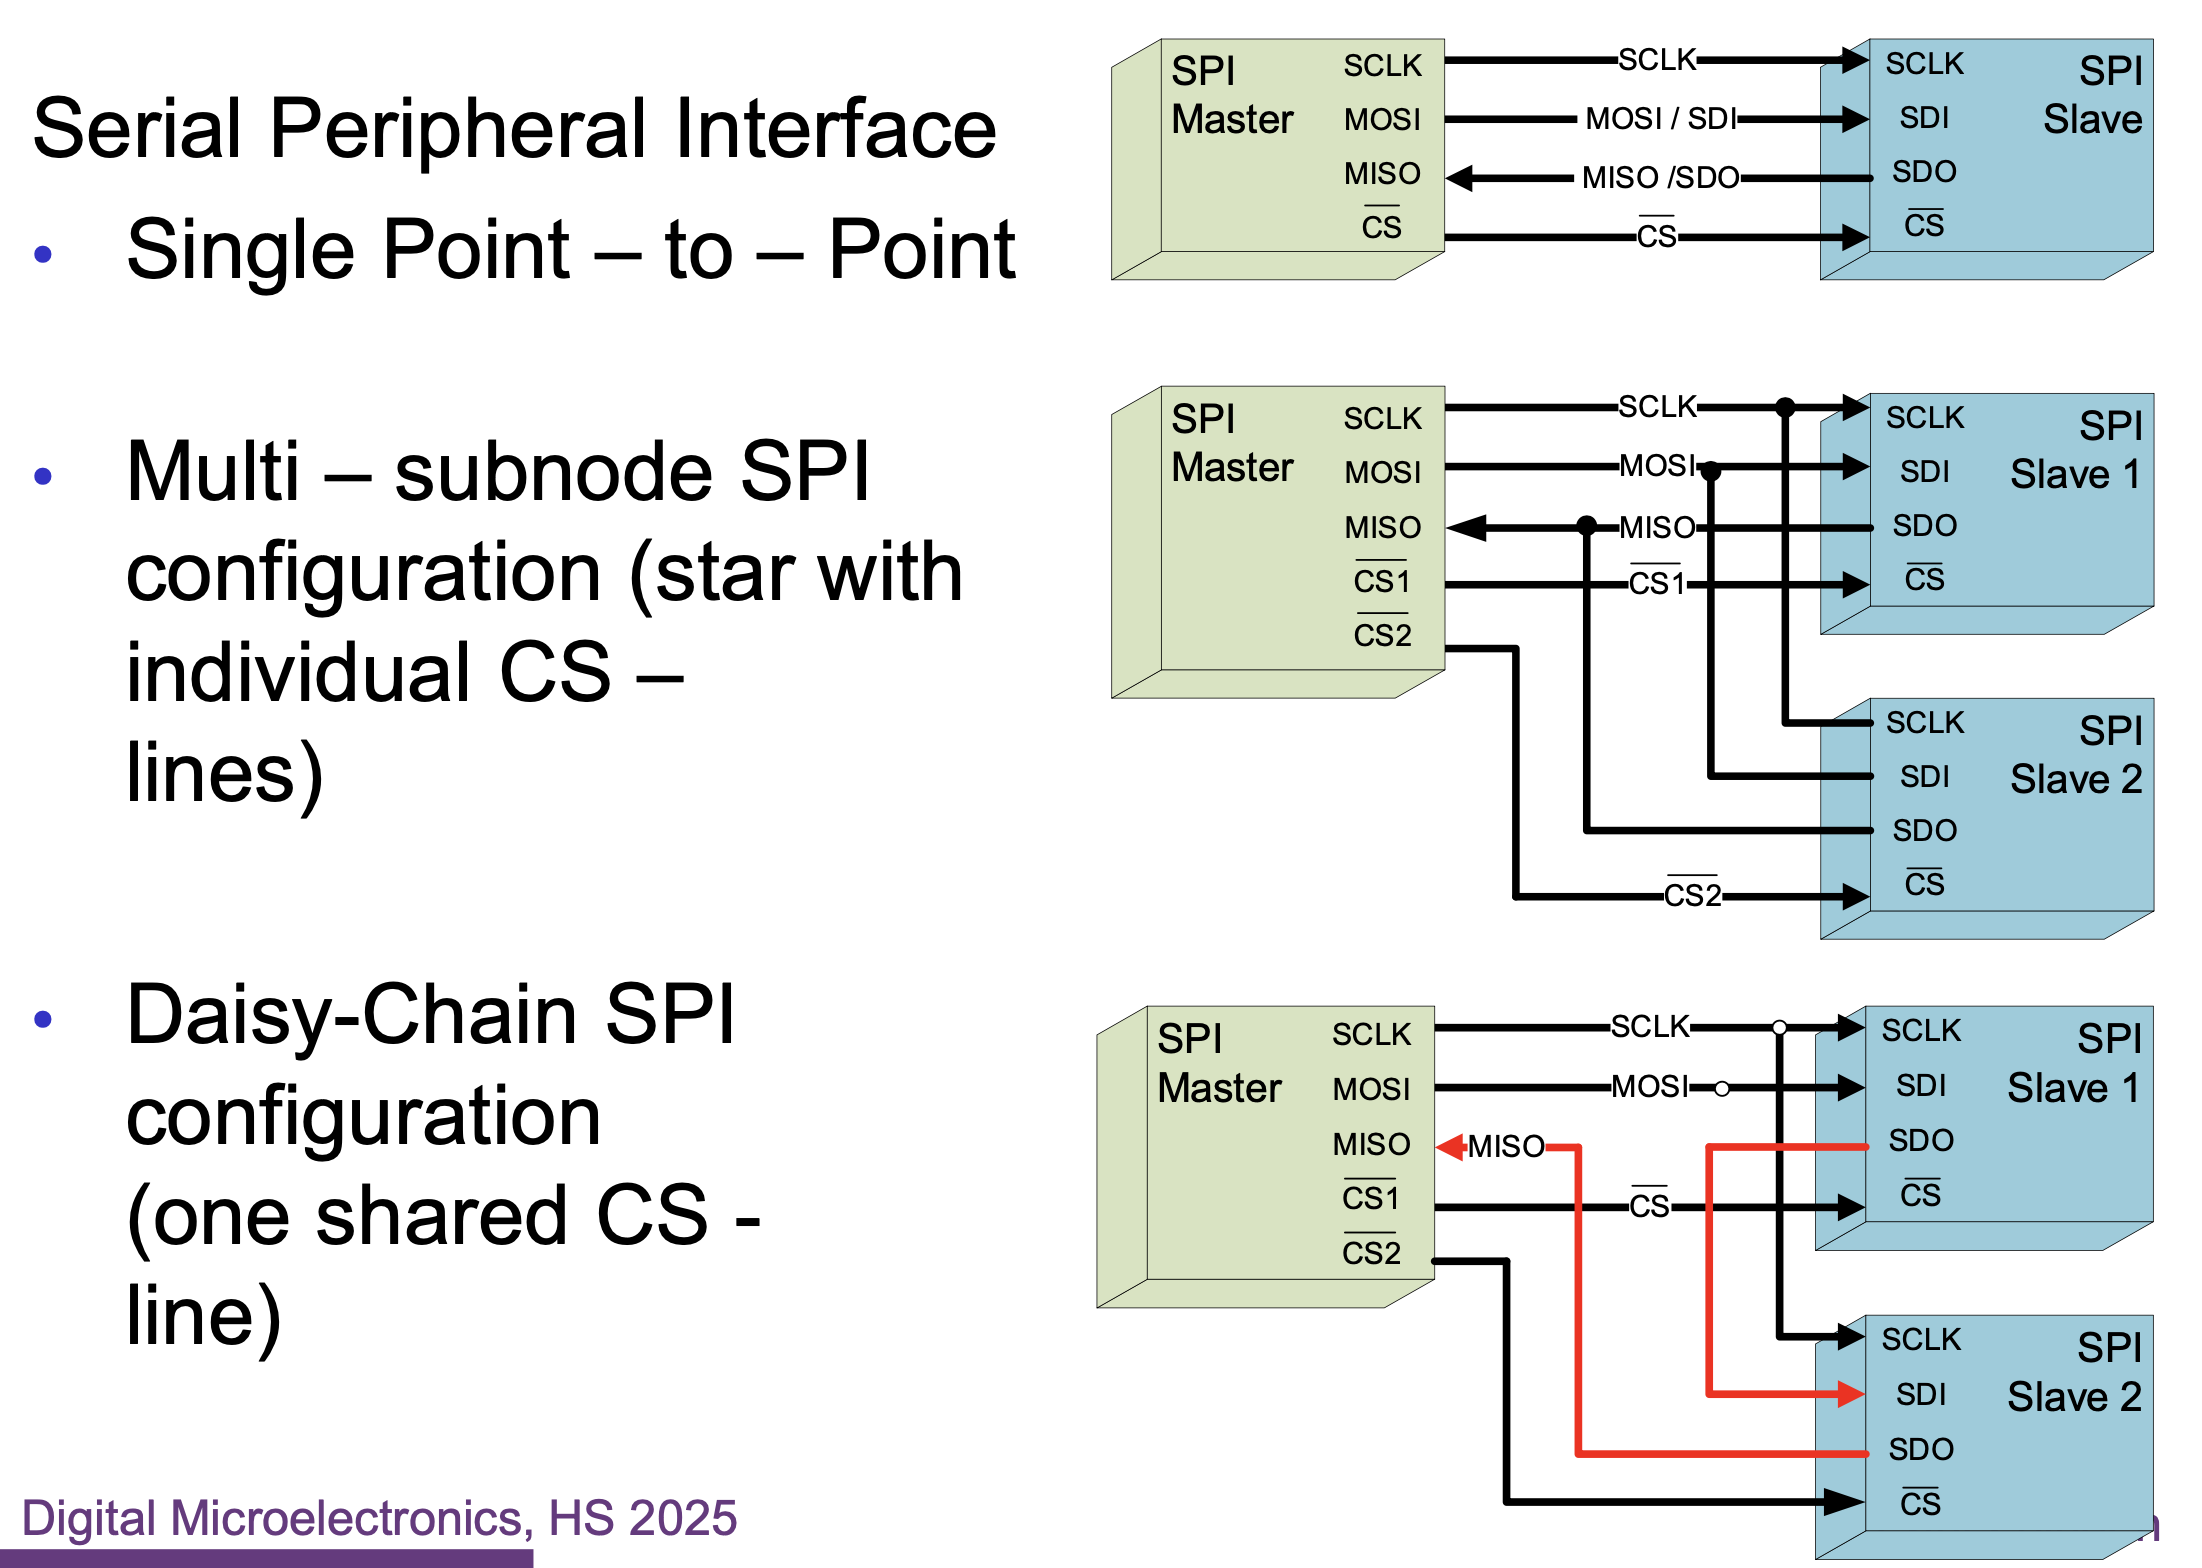
\includegraphics[width=\linewidth,height=0.24\textheight,keepaspectratio]{fig/L6_spi_topology.png}
  \caption{SPI-Topologien, Signale und Master-Slave-Prinzip.}
\end{figure}

\subsection{SPI-Hardwarestruktur}
Ein SPI-System besteht aus:
\begin{itemize}
  \item TX-Shiftregister
  \item RX-Shiftregister
  \item Clock-Divider
  \item FSM
\end{itemize}

\imp{Prüfungsregel:}  
\hilite{SPI} ist \hilite{vollständig} \hilite{synchron}.

\subsection{SPI-Beschreibung in VHDL}
Die Beschreibung folgt einem festen Muster:
\begin{itemize}
  \item Generics für Wortbreite und Mode
  \item FSM (Idle, Load, Shift, Done)
  \item SCLK aus Clock-Divider
\end{itemize}

\subsection{I\textsuperscript{2}C – Inter-Integrated Circuit}
I\textsuperscript{2}C ist eine synchrone Zweidraht-Bus-Schnittstelle.

Eigenschaften:
\begin{itemize}
  \item SDA, SCL
  \item Multi-Master, Multi-Slave
  \item Open-Drain
\end{itemize}

\subsection{I\textsuperscript{2}C-Protokoll und Timing}
Merkmale:
\begin{itemize}
  \item Start: SDA fällt bei SCL = High
  \item Stop: SDA steigt bei SCL = High
  \item Datenwechsel nur bei SCL = Low
\end{itemize}

Nach 8 Bit folgt ein Acknowledge-Zyklus.

\begin{figure}[t]
  \centering
  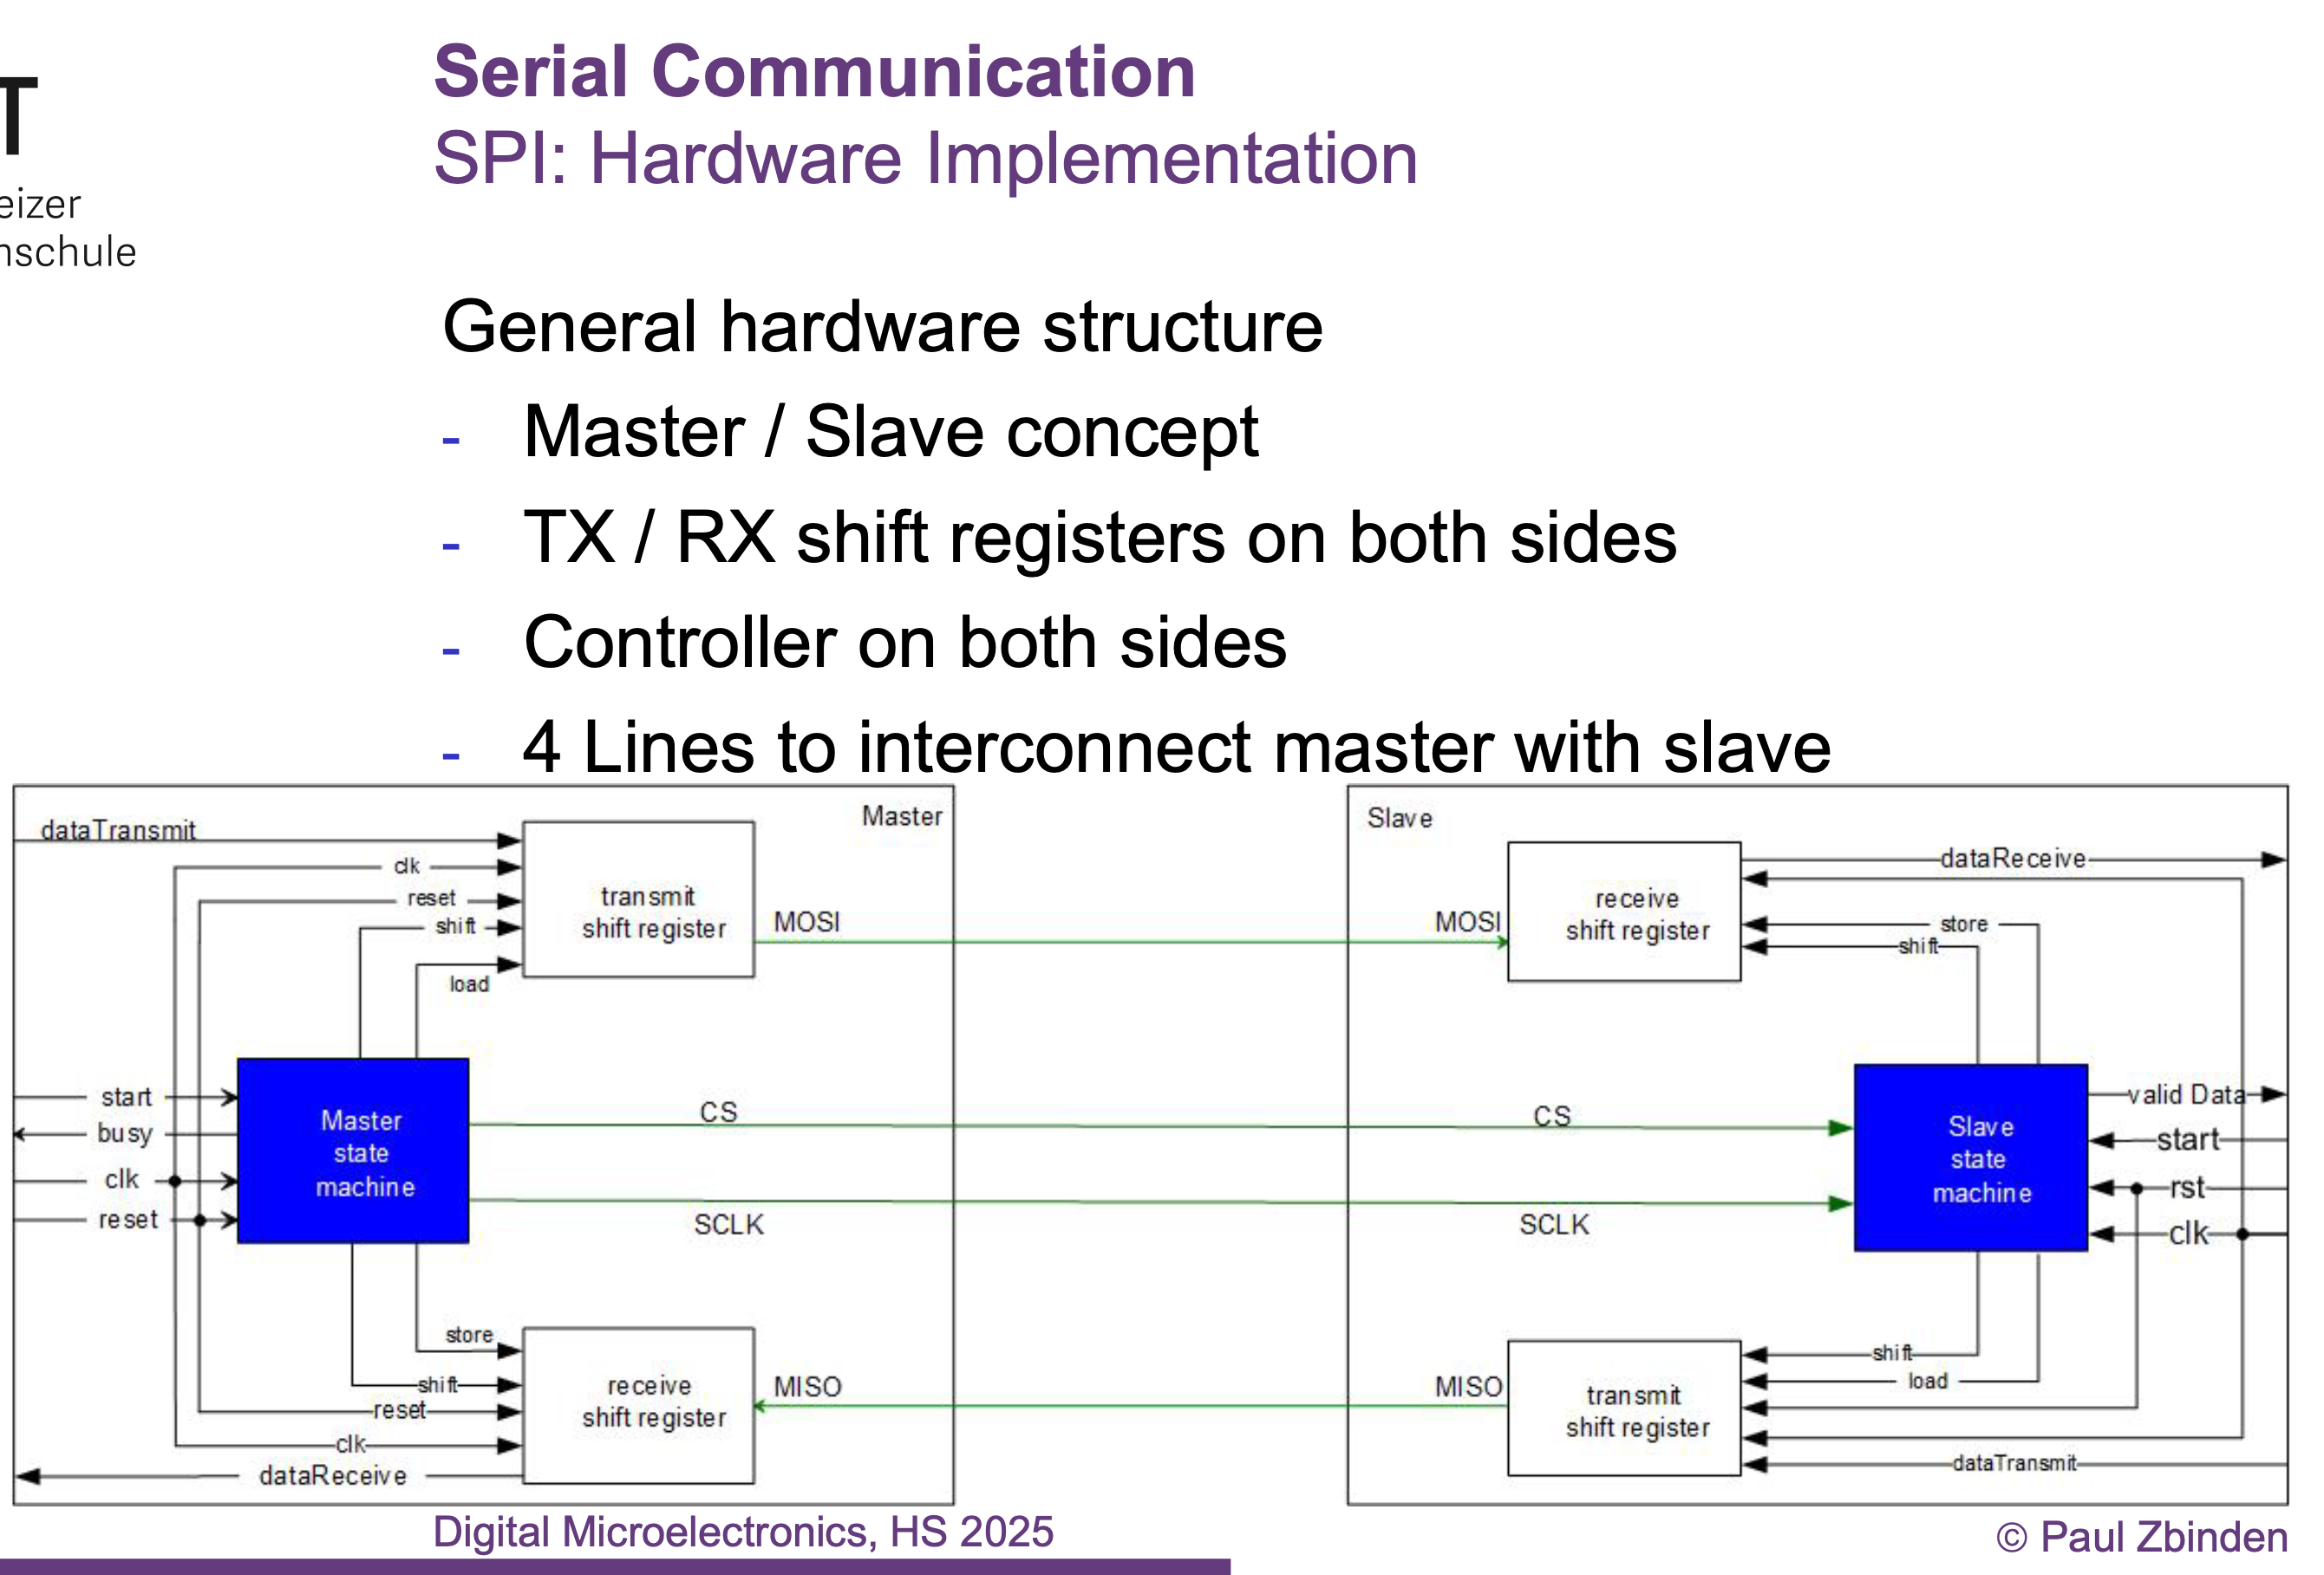
\includegraphics[width=\linewidth,height=0.24\textheight,keepaspectratio]{fig/L6_i2c_timing.png}
  \caption{I\textsuperscript{2}C Timingdiagramm mit Start/Stop/Acknowledge.}
\end{figure}

\subsection{I\textsuperscript{2}C-Hardware und Arbitration}
Durch Wired-AND-Struktur ist Arbitration möglich:
\begin{itemize}
  \item Mehrere Master dürfen senden
  \item Master verliert, wenn er '1' sendet und '0' liest
\end{itemize}

Open-Drain in VHDL:
\begin{lstlisting}[emph={entity,architecture,process,rising_edge,signal,constant,generic,port},emphstyle=\bfseries\color{codeemph}][emph={entity,architecture,process,rising_edge,signal,constant,generic,port},emphstyle=\bfseries\color{codeemph}]
sda <= '0' when drive_low='1' else 'Z';
\end{lstlisting}

\subsection{UART (Einordnung)}
UART ist eine asynchrone Punkt-zu-Punkt-Schnittstelle.

Eigenschaften:
\begin{itemize}
  \item Keine gemeinsame Clock
  \item Start- und Stop-Bits
  \item Einfache Hardware
\end{itemize}

\imp{Abschluss-Merksatz:}  
\hilite{UART} ist \hilite{einfach}, \hilite{aber} unpräzise und langsam.



% ============================================================
\section{Parallel On-Chip Communication}

\subsection{Einordnung paralleler Kommunikation}
Parallele Kommunikation überträgt mehrere Bits gleichzeitig über separate Leitungen.  
Sie wird primär \textbf{on-chip} eingesetzt, da physikalische Effekte off-chip die Skalierbarkeit stark begrenzen.

\imp{Merksatz (Prüfung):}  
\hilite{Parallel} = \hilite{hoher} \hilite{Durchsatz} bei kurzer Distanz.

\subsection{Serial vs. Parallel}
Serielle Kommunikation überträgt ein Bit pro Leitung und benötigt Serialisierung und Deserialisierung.  
Parallele Kommunikation überträgt $N$ Bits gleichzeitig.

\begin{itemize}
  \item \textbf{Seriell}: wenige Leitungen, SERDES, höhere Latenz
  \item \textbf{Parallel}: viele Leitungen, einfache Logik, hoher Durchsatz
\end{itemize}

\imp{Prüfungsregel:}  
\hilite{Off-chip} \hilite{dominiert} \hilite{seriell}, on-chip dominiert parallel.

\begin{figure}[t]
  \centering
  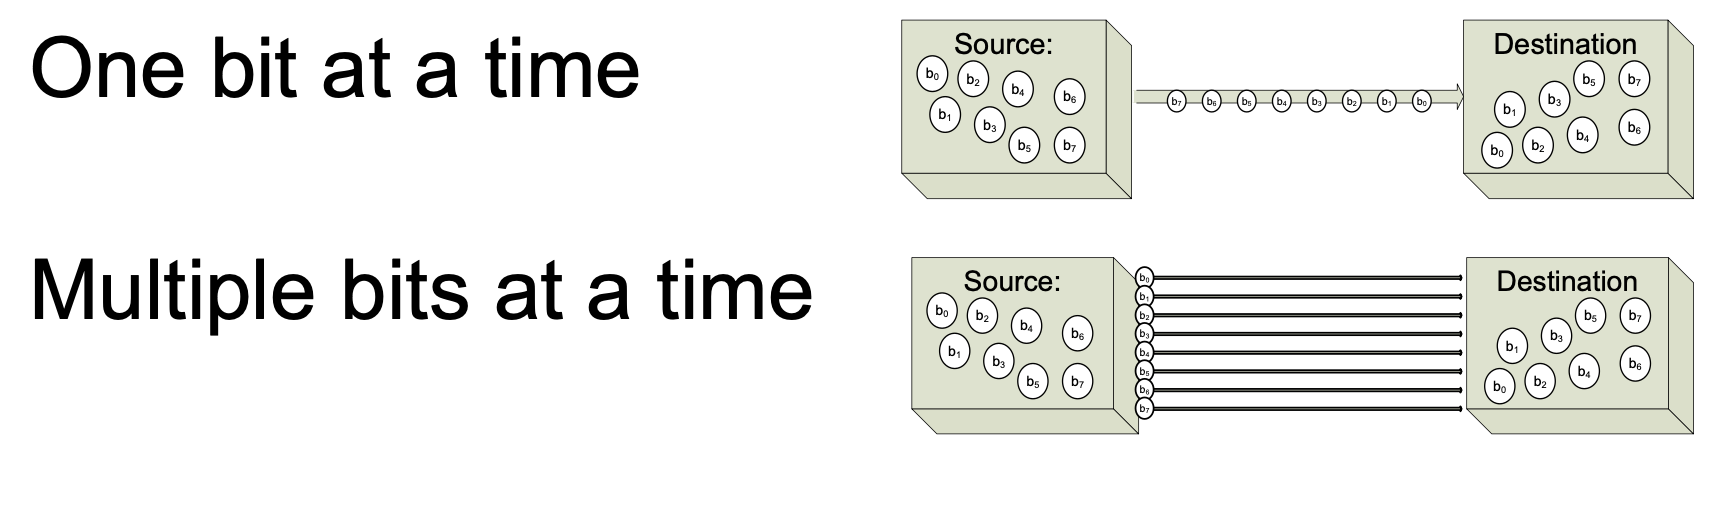
\includegraphics[width=\linewidth,height=0.22\textheight,keepaspectratio]{fig/L7_serial_vs_parallel.png}
  \caption{Serial vs. Parallel Kommunikation auf Bit-Ebene.}
\end{figure}

\subsection{Physikalische Grenzen paralleler Off-Chip-Kommunikation}
Außerhalb des Chips begrenzen physikalische Effekte den Nutzen paralleler Übertragung:

\begin{itemize}
  \item \textbf{Skew}: Laufzeitunterschiede zwischen Leitungen
  \item \textbf{Crosstalk}: Kopplung benachbarter Leitungen
  \item Hoher Pad-Bedarf
  \item Hohe Kosten
\end{itemize}

\imp{Prüfungsregel:}  
\hilite{Mehr} \hilite{Leitungen} $\rightarrow$ \hilite{mehr} Off-Chip-Probleme.

\subsection{Vorteile paralleler On-Chip-Kommunikation}
Auf dem Chip entfallen die meisten Nachteile:

\begin{itemize}
  \item Keine Pads
  \item Kurze, kontrollierte Leitungen
  \item Geringer Skew
  \item Keine SERDES-Strukturen
\end{itemize}

\textbf{Merksatz:}  
\hilite{On-Chip-}\hilite{Interconnect}s sind \hilite{natürlich} parallel.

\subsection{Grundstruktur paralleler Schnittstellen}
Eine parallele Schnittstelle besteht aus:

\begin{itemize}
  \item Datenbus
  \item Steuerleitungen (Read, Write, Valid, Ready)
  \item Gemeinsamer Clock
\end{itemize}

\imp{Prüfungsregel:}  
\hilite{Parallele} \hilite{Interfaces} sind immer \hilite{synchron}.

\subsection{AXI als Standard-On-Chip-Interconnect}
AXI (Advanced eXtensible Interface) ist Teil der AMBA-Architektur von ARM und de-facto Standard für SoC-Designs.

\begin{itemize}
  \item Master-Slave
  \item Memory-Mapped
  \item Hohe Parallelität
\end{itemize}

\imp{Merksatz (Prüfung):}  
\hilite{AXI} ist \hilite{kanalbasiert}, kein \hilite{klassischer} Bus.

\subsection{AXI-Architektur}
AXI verwendet fünf unabhängige Kanäle:

\begin{itemize}
  \item Write Address (AW)
  \item Write Data (W)
  \item Write Response (B)
  \item Read Address (AR)
  \item Read Data (R)
\end{itemize}

\imp{Prüfungsregel:}  
\hilite{Read} und \hilite{Write} sind \hilite{vollständig} getrennt.

\begin{figure}[t]
  \centering
  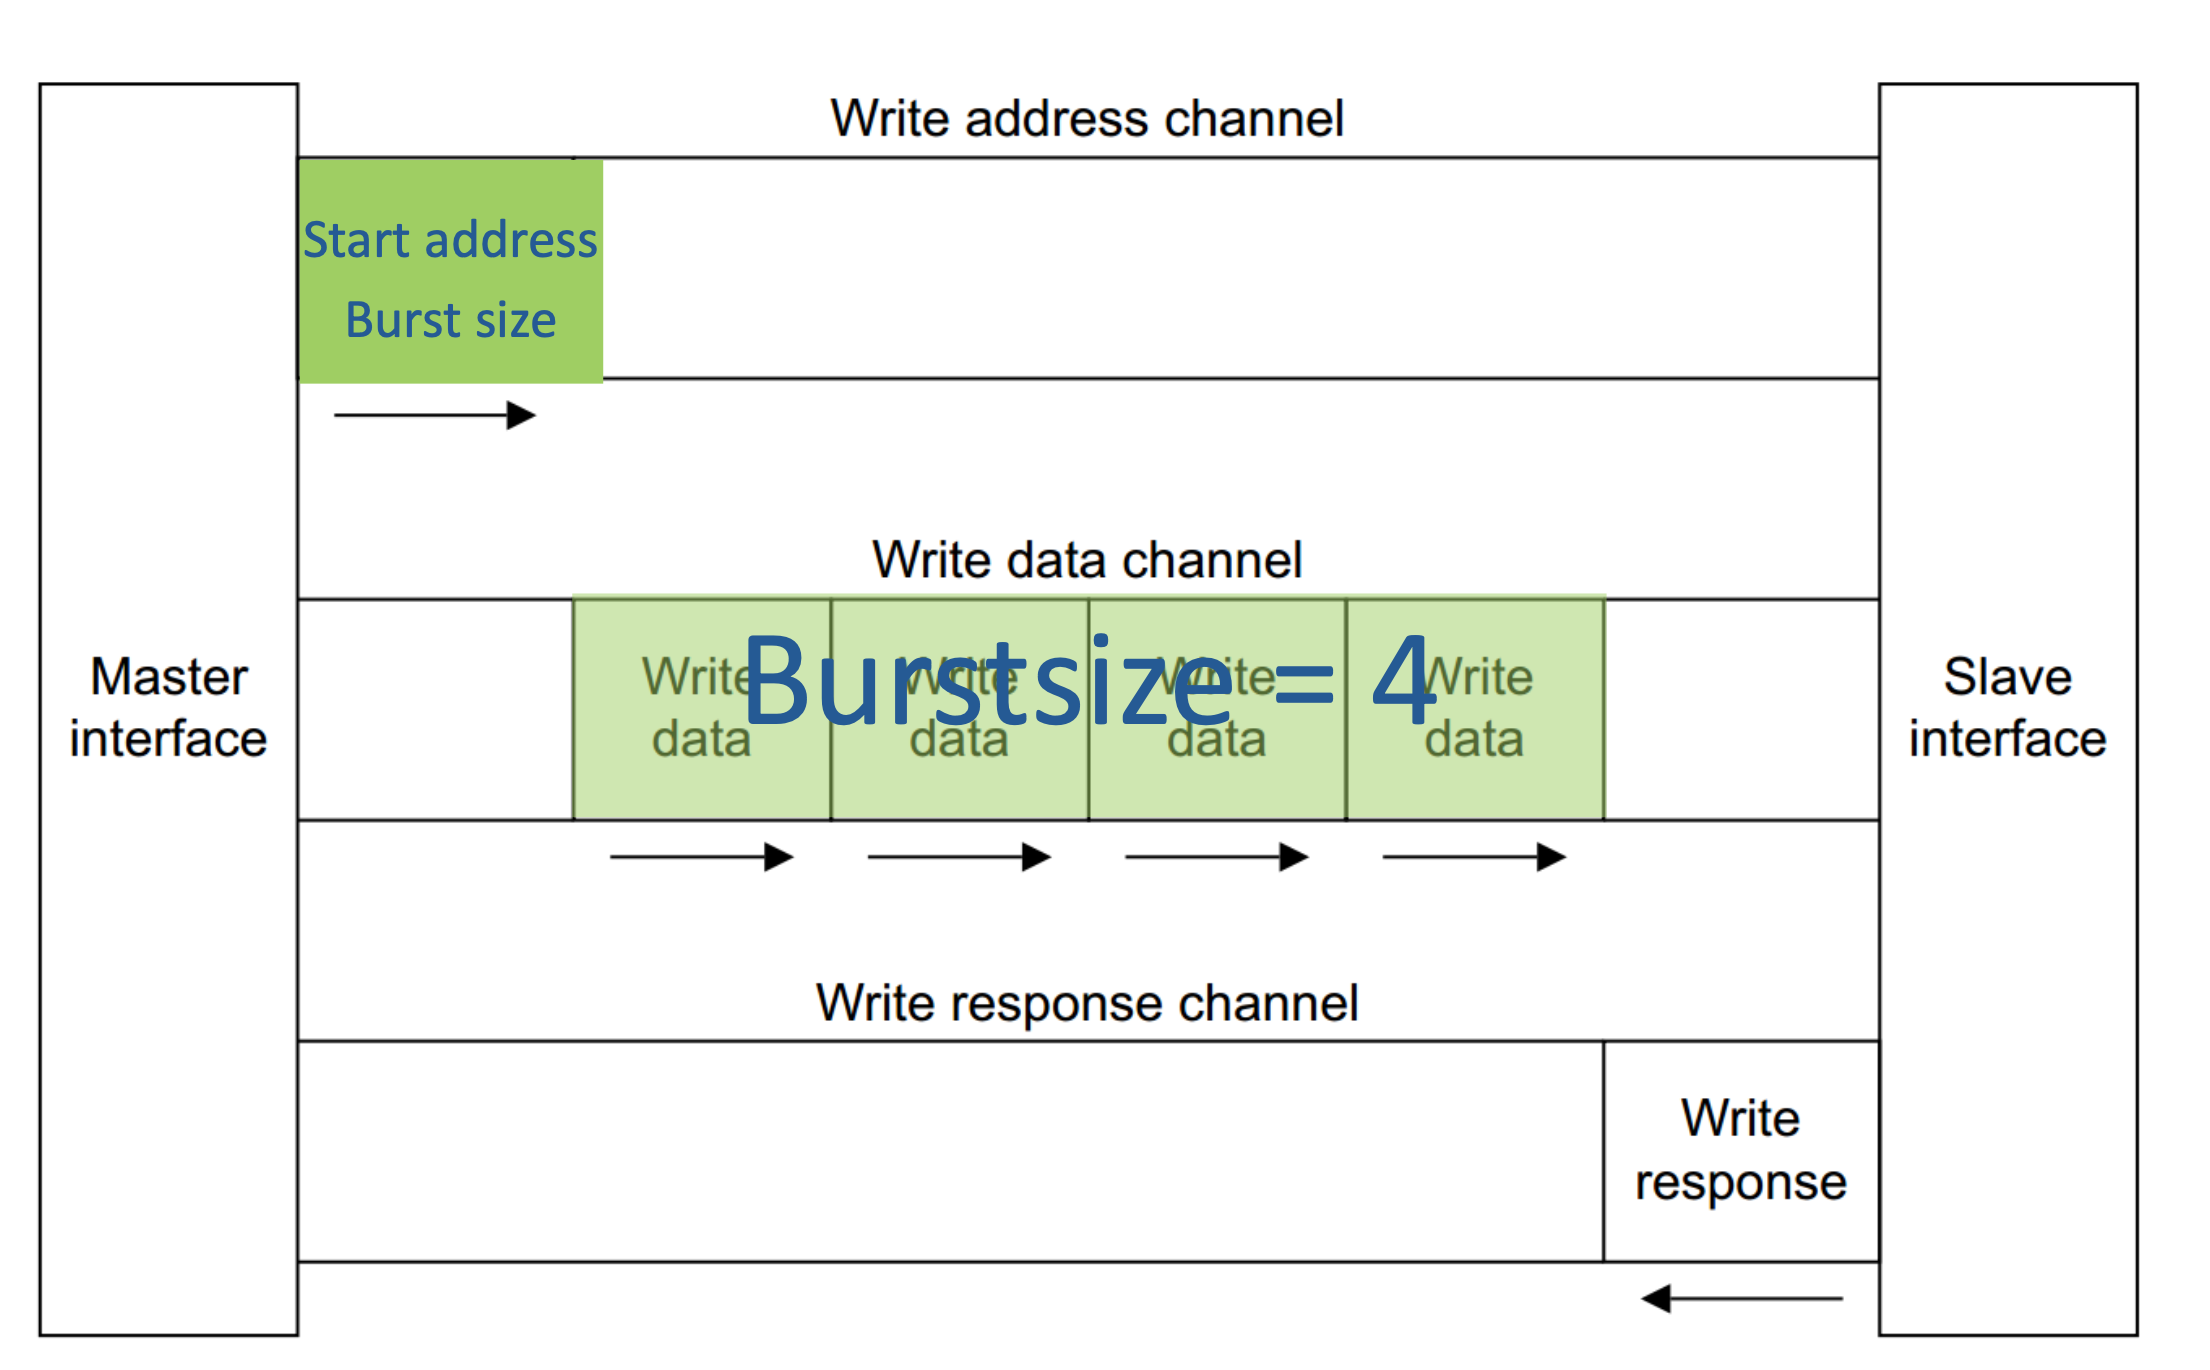
\includegraphics[width=\linewidth,height=0.22\textheight,keepaspectratio]{fig/L7_axi_5channels.png}
  \caption{AXI Fünf-Kanal-Architektur für Read/Write.}
\end{figure}

\subsection{AXI-Handshake-Prinzip}
Jeder Kanal nutzt dasselbe Handshake-Verfahren.

\begin{itemize}
  \item Sender setzt \texttt{VALID}
  \item Empfänger setzt \texttt{READY}
  \item Transfer bei \texttt{VALID} \& \texttt{READY}
\end{itemize}

\imp{Zentrale Regel (Prüfung):}  
\hilite{Daten} müssen stabil bleiben, solange \hilite{\texttt{VALID=1} und \texttt{\hilite{READY}=0}}.

\begin{figure}[t]
  \centering
  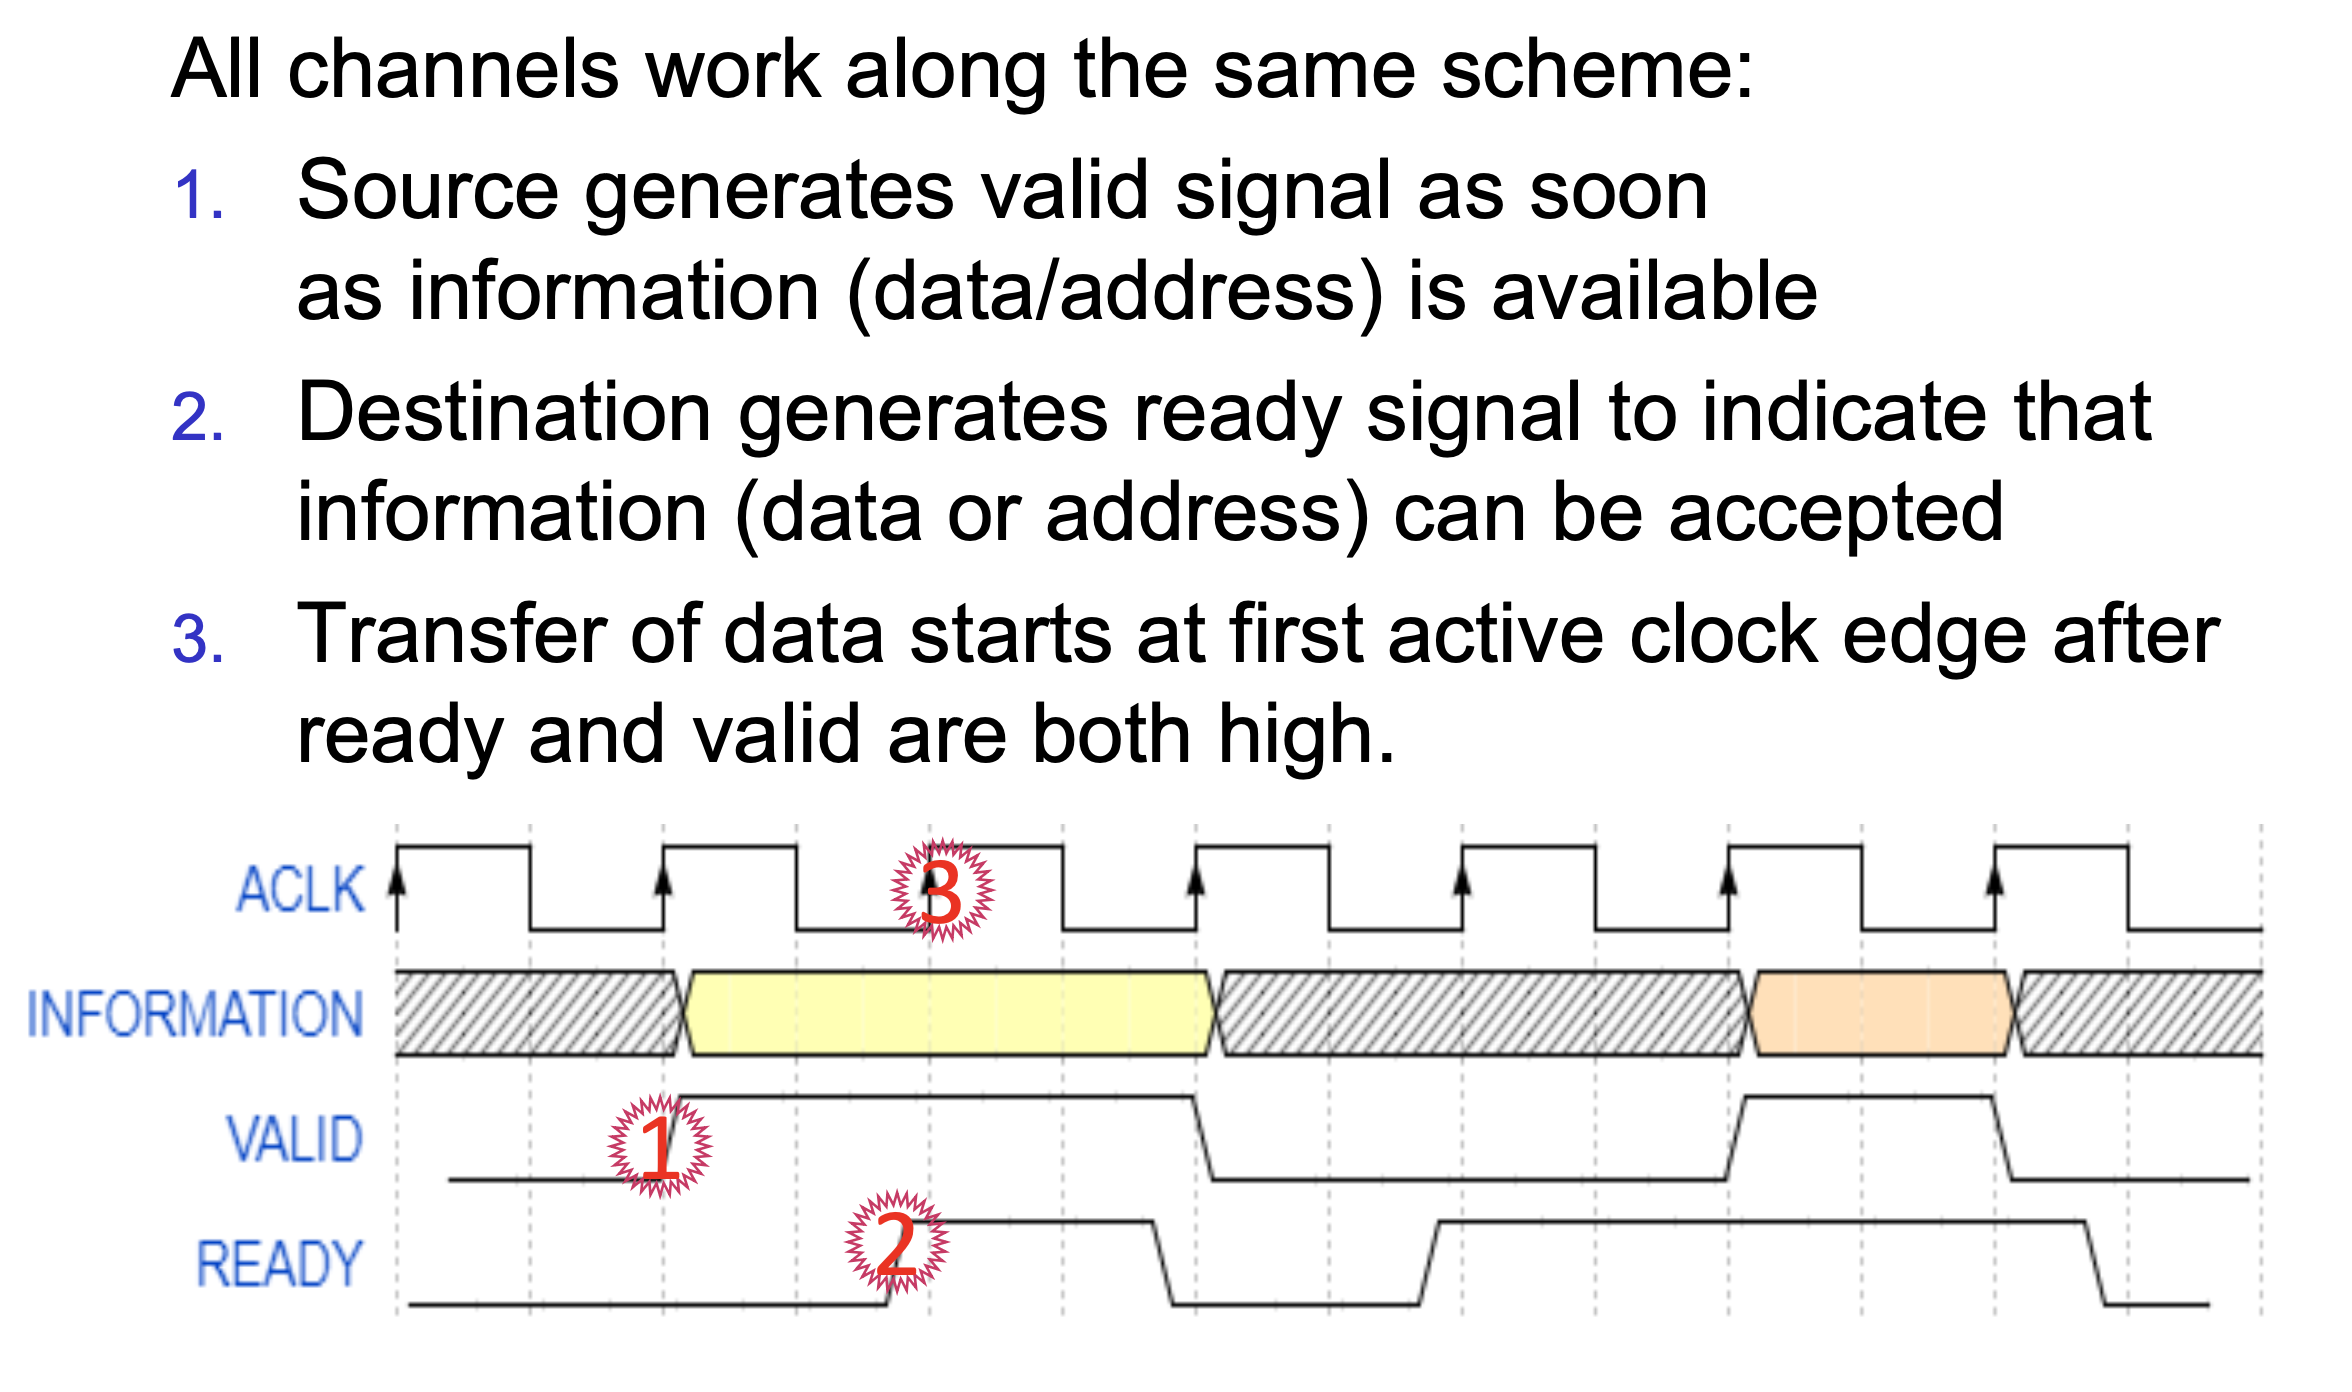
\includegraphics[width=\linewidth,height=0.22\textheight,keepaspectratio]{fig/L7_axi_handshake.png}
  \caption{AXI Handshake Timingdiagramm (VALID/READY).}
\end{figure}

\subsection{AXI-Varianten}
AXI existiert in mehreren Varianten:

\begin{itemize}
  \item \textbf{AXI4}: Vollständig, Bursts bis 256 Transfers
  \item \textbf{AXI4-Lite}: Keine Bursts, Registerzugriffe
  \item \textbf{AXI4-Stream}: Datenstrom ohne Adressen
\end{itemize}

\imp{Prüfungsregel:}  
\hilite{Register-}\hilite{IP} $\rightarrow$ \hilite{AXI4-Lite}.

\subsection{AXI-Interconnects}
Unterstützte Topologien:

\begin{itemize}
  \item 1-to-1
  \item N-to-1 (Arbitration)
  \item 1-to-M (Address-Decoding)
  \item N-to-M
\end{itemize}

\begin{figure}[t]
  \centering
  \begin{subfigure}[t]{0.49\linewidth}
    \centering
    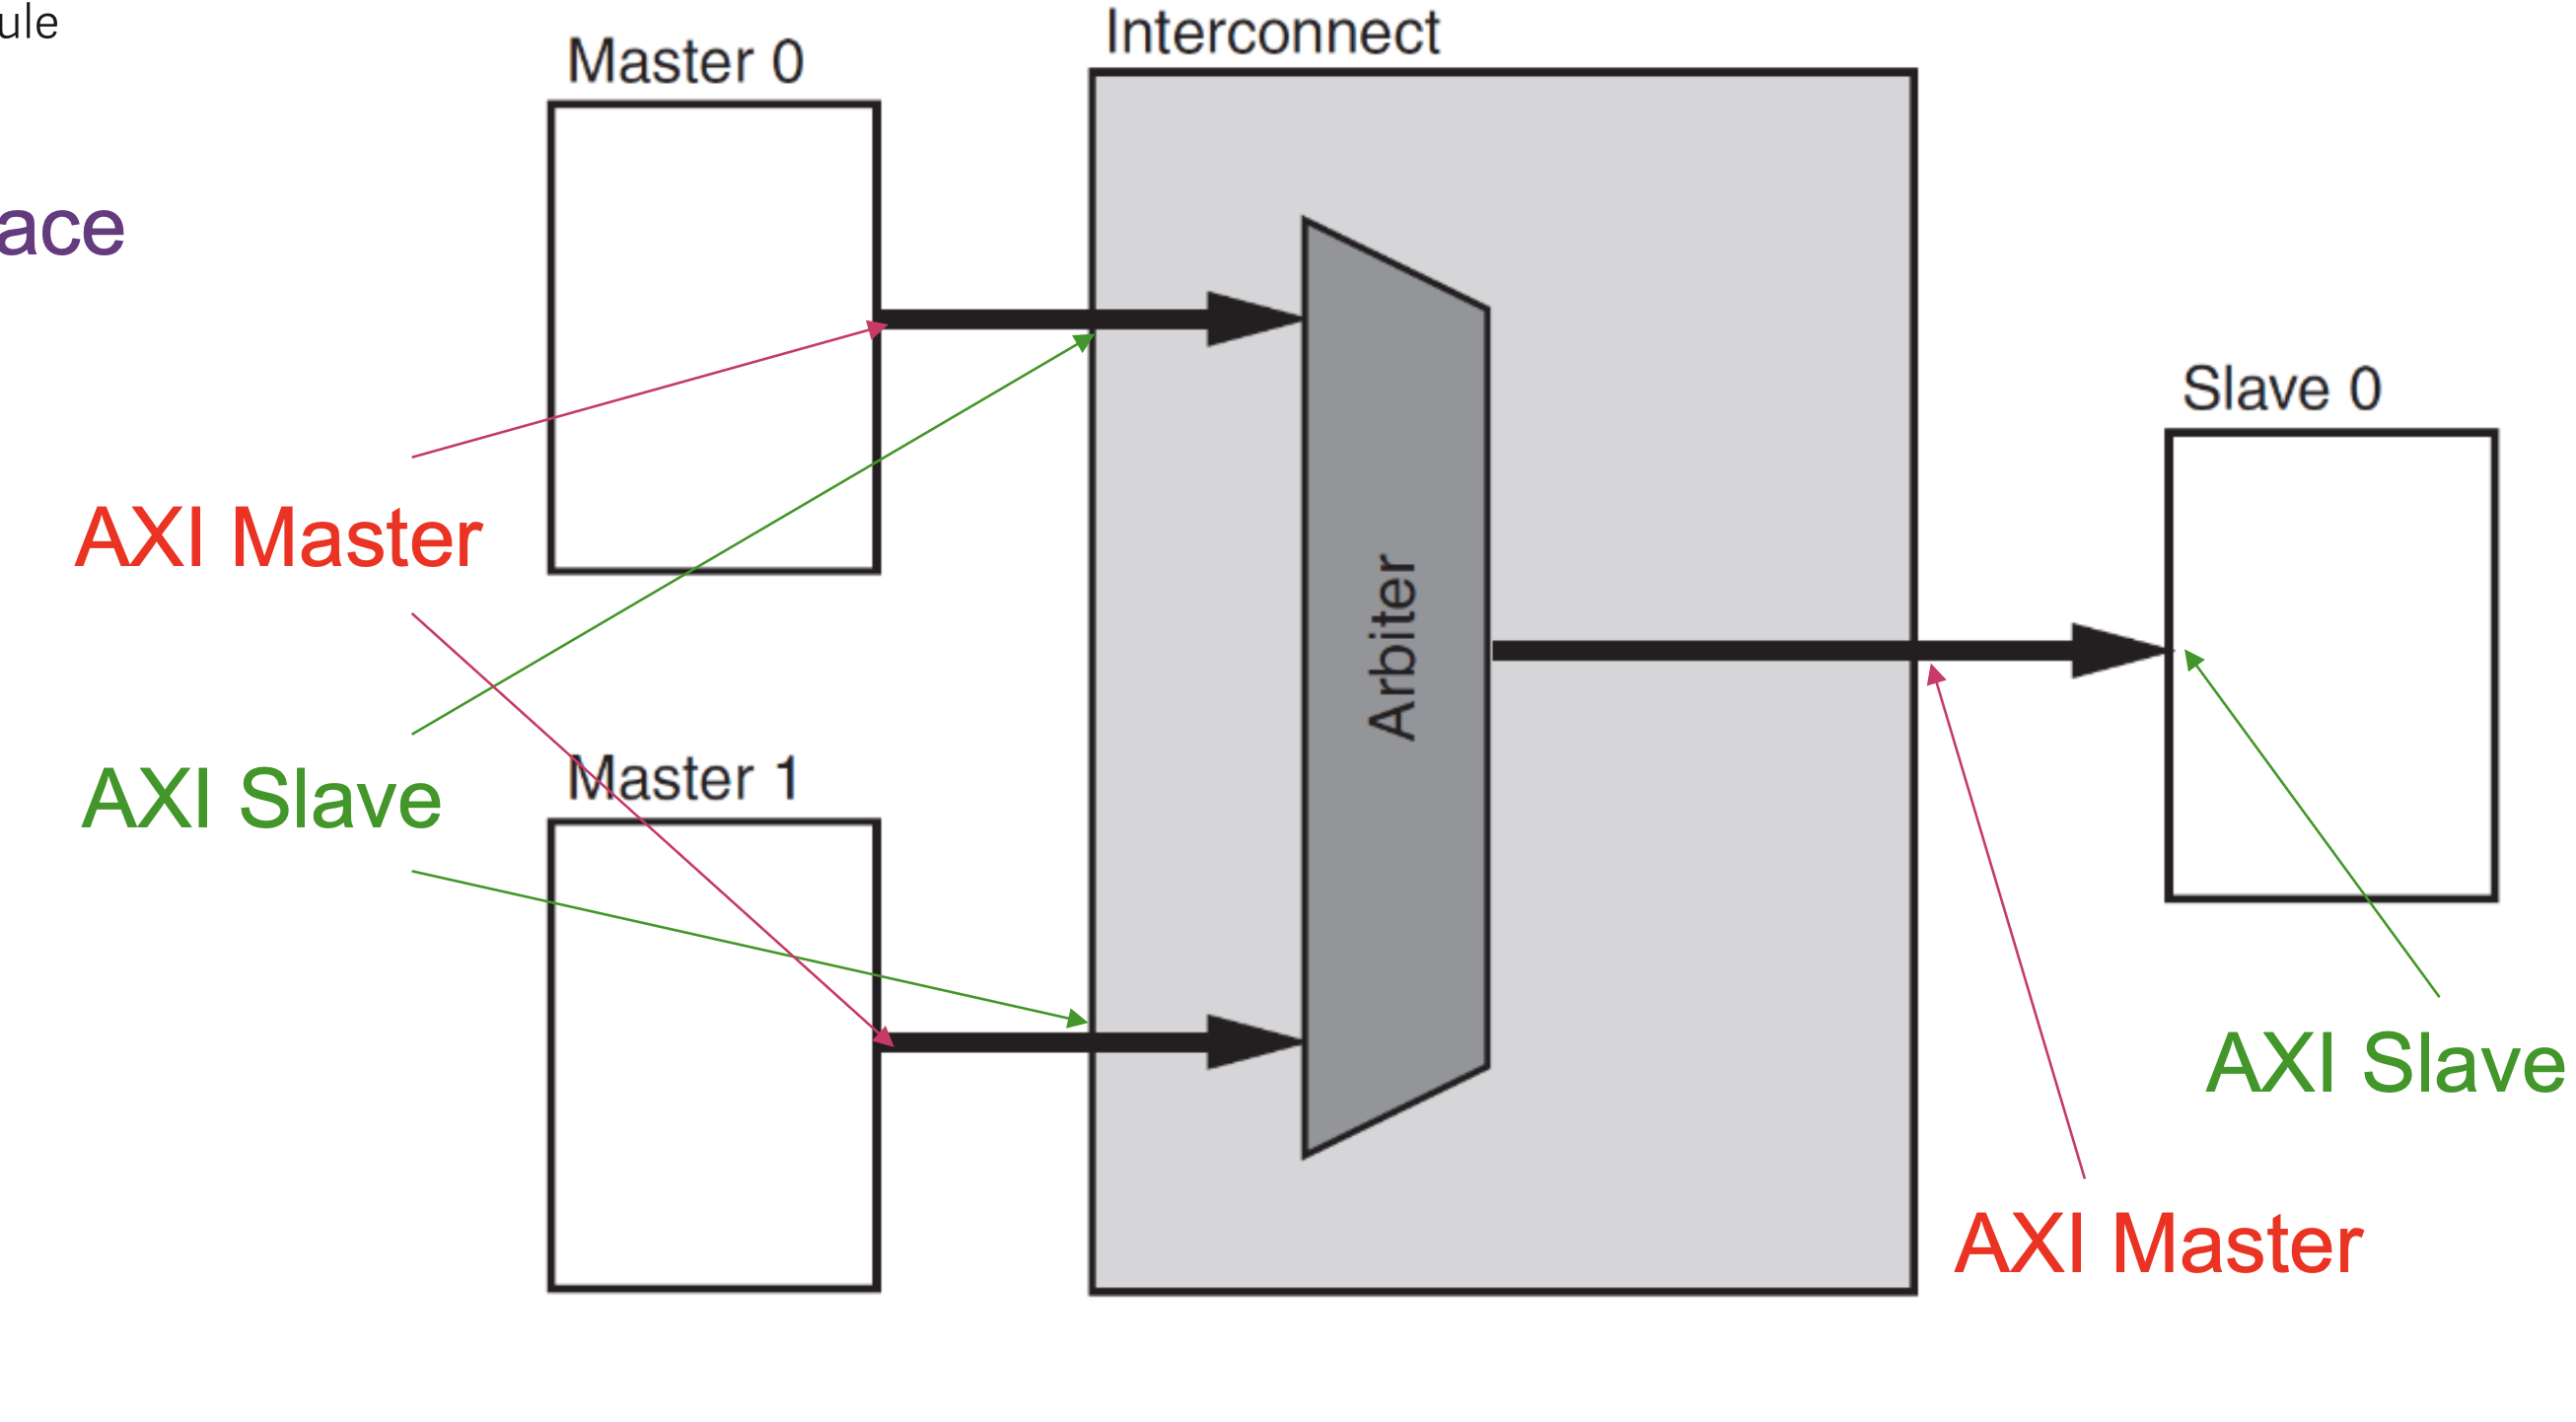
\includegraphics[width=\linewidth,height=0.20\textheight,keepaspectratio]{fig/L7_axi_interconnect_n_to_1.png}
    \caption{N-to-1 (Arbitration).}
  \end{subfigure}\hfill
  \begin{subfigure}[t]{0.49\linewidth}
    \centering
    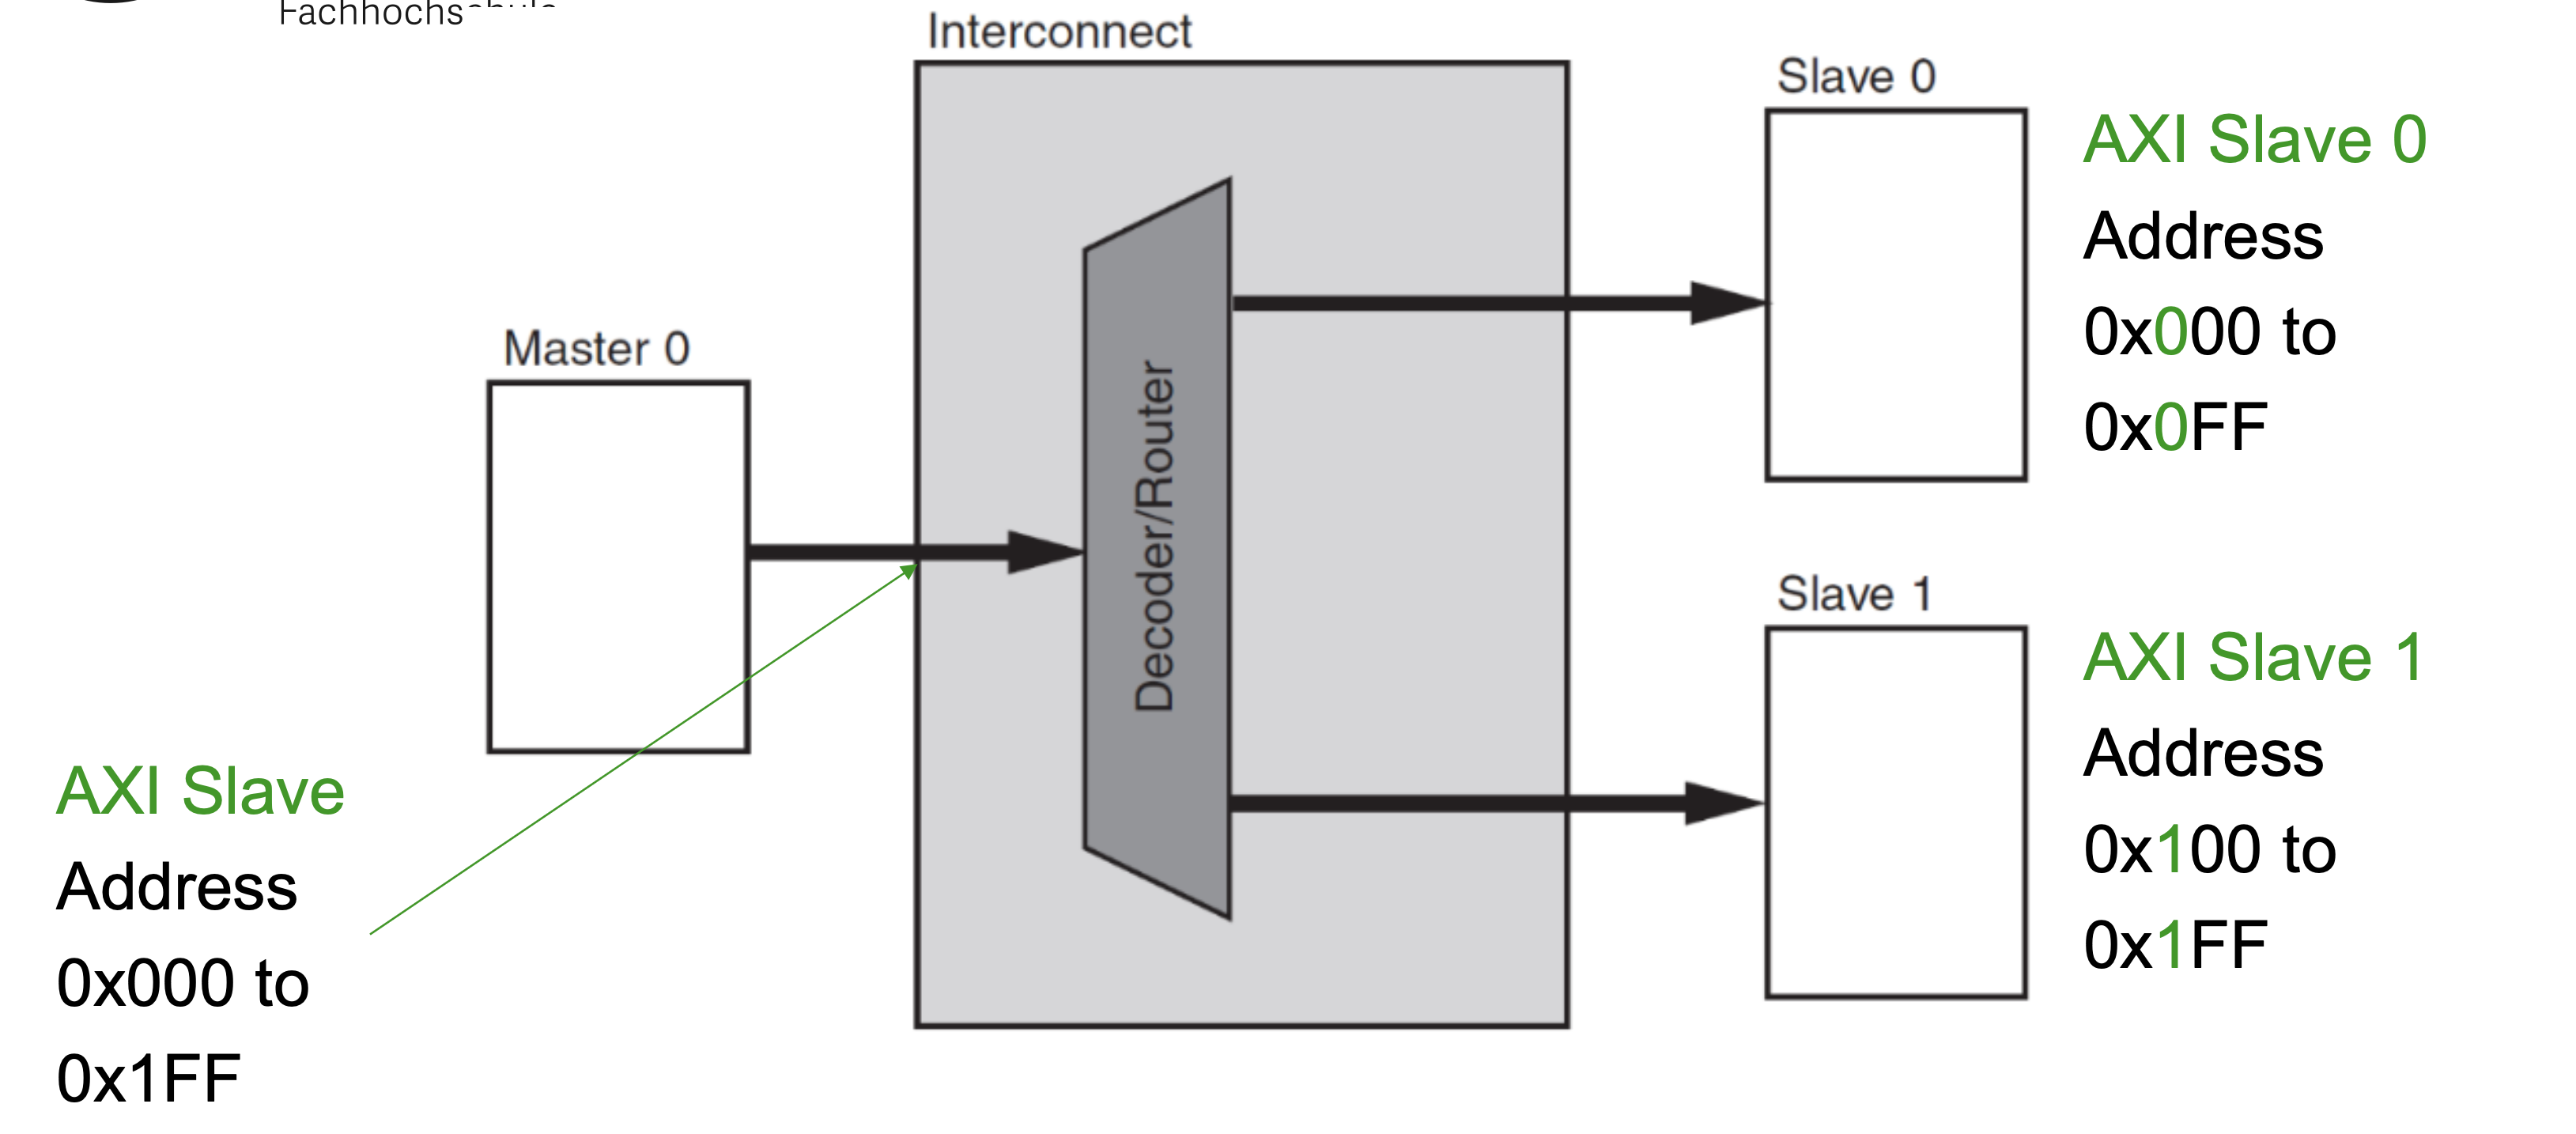
\includegraphics[width=\linewidth,height=0.20\textheight,keepaspectratio]{fig/L7_axi_interconnect_1_to_m.png}
    \caption{1-to-M (Decoding/Routing).}
  \end{subfigure}
  \caption{AXI Interconnect Topologien: N-to-1 und 1-to-M.}
\end{figure}

\subsection{AXI auf Zynq}
Der Zynq-SoC bietet mehrere AXI-Schnittstellen zwischen Processing System (PS) und Programmable Logic (PL):

\begin{itemize}
  \item General Purpose (GP)
  \item High Performance (HP)
  \item Accelerator Coherency Port (ACP)
\end{itemize}

\begin{figure}[t]
  \centering
  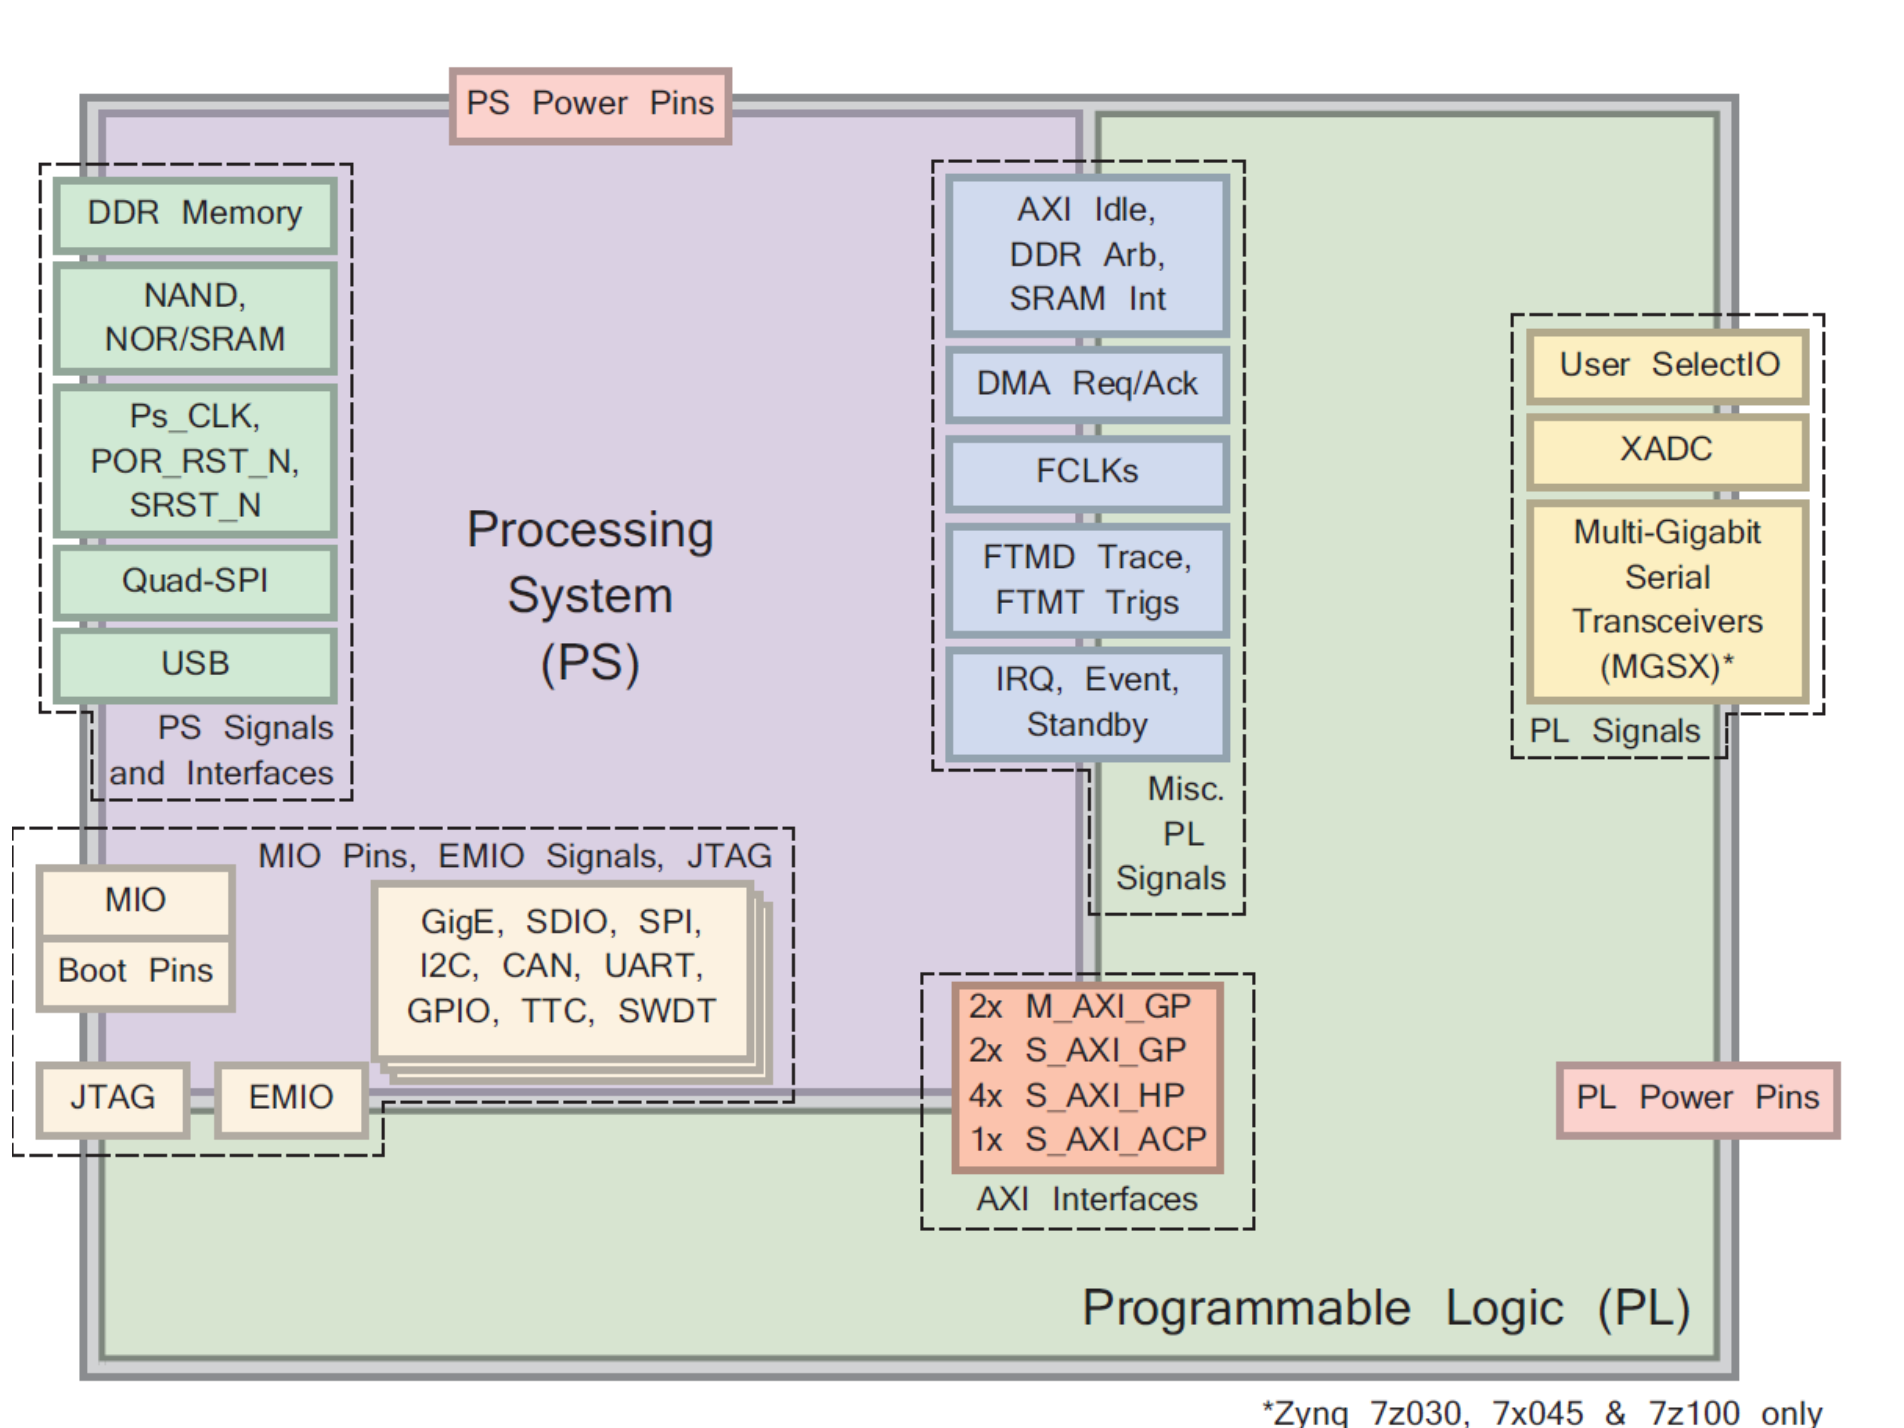
\includegraphics[width=\linewidth,height=0.22\textheight,keepaspectratio]{fig/L7_zynq_ps_pl_axi.png}
  \caption{Zynq PS--PL AXI-Übersicht.}
\end{figure}

\subsection{AXI3 vs. AXI4}
Im Zynq:
\begin{itemize}
  \item PS nutzt AXI3
  \item Xilinx-IP nutzt AXI4
\end{itemize}

\imp{Prüfungsregel:}  
\hilite{Protokollkonverter} \hilite{lösen} \hilite{Inkompatibilitäten}.

\subsection{AXI-IP-Erstellung}
Gängige Vorgehensweisen:
\begin{itemize}
  \item Separater AXI-Interface-Block + User-Logik
  \item AXI-Peripheral-Template
\end{itemize}

\subsection{Register-basierte Kommunikation}
Kommunikation erfolgt über Memory-Mapped Register:

\begin{itemize}
  \item CPU schreibt Register
  \item Logik liest Register
  \item Logik schreibt Status
  \item CPU liest Status
\end{itemize}

\subsection{FPGA–Processor-Kommunikation}
Integration erfolgt über:
\begin{itemize}
  \item Hardware-Export
  \item BSP-Generierung
  \item Automatische Address-Header
\end{itemize}

\imp{Abschluss-Merksatz:}  
\hilite{AXI} \hilite{verbindet} \hilite{Software-Welt} und FPGA-Logik deterministisch.



% ============================================================
\section{Debugging and Verification of SoC}

\subsection{Einordnung der Verifikation}
Design Verification ist ein zentraler Bestandteil moderner SoC-Entwicklung und beansprucht häufig über 50\,\% der Entwicklungszeit.

\imp{Prüfungsmerksatz:}  
\hilite{Verifikation} \hilite{prüft} \emph{richtiges Verhalten}, nicht Performance oder \hilite{Timing}.

In dieser Vorlesung wird ausschließlich \textbf{funktionale Verifikation} betrachtet.

\subsection{Funktionale Verifikation}
Funktionales Verhalten lässt sich beschreiben als:
\[
y = f(x, \text{state})
\]

\imp{Prüfungsregel:}  
\hilite{Verifikation} \hilite{prüft}, ob für \hilite{gegebene} Eingänge und Zustände die korrekten Ausgänge entstehen.

\subsection{Exhaustive Verification}
Exhaustive Verification testet \textbf{alle möglichen Eingangskombinationen}.

\subsubsection*{\textcolor{codeemph}{Prüfungsformel}}
Für $n$ unabhängige Eingänge gilt:
\[
N = 2^n
\]

\imp{Prüfungsregel:}  
\hilite{Exhaustive} \hilite{Verification} ist \hilite{theoretisch} korrekt, praktisch unmöglich.

\subsection{Pragmatische Verifikationsstrategie}
Da Exhaustive Verification nicht realisierbar ist, wird ein Kompromiss gewählt:

\begin{itemize}
  \item Assertion-Based Verification
  \item Gezielte Testfälle
  \item Zufällige Stimuli
  \item Trennung von Design und Test
\end{itemize}

\textbf{Merksatz:}  
\hilite{Ziel} ist \hilite{hohe} \hilite{Fehlerabdeckung}, nicht Vollständigkeit.

\subsection{Assertion-Based Verification}
Assertions sind eingebaute Konsistenzprüfungen.

\subsubsection*{Typische Assertions}
\begin{itemize}
  \item Illegale FSM-Zustände
  \item Ungültige Adressen
  \item Über- und Unterläufe
\end{itemize}

\subsubsection*{Assertion – Code-Beispiel}
\begin{lstlisting}[emph={entity,architecture,process,rising_edge,signal,constant,generic,port},emphstyle=\bfseries\color{codeemph}][emph={entity,architecture,process,rising_edge,signal,constant,generic,port},emphstyle=\bfseries\color{codeemph}]
assert addr < MAX_ADDR
  report "Address out of range"
  severity error;
\end{lstlisting}

\imp{Prüfungsregel:}  
\hilite{Assertions} sind nicht für die \hilite{Synthese} \hilite{bestimmt}.

\subsection{Testfälle und Stimuli}
Effektive Testfälle decken unterschiedliche Szenarien ab:

\begin{itemize}
  \item Normalbetrieb
  \item Grenzfälle
  \item Fehlerfälle
  \item Zufällige Daten
\end{itemize}

\imp{Prüfungsregel:}  
\hilite{Grenzwerte} \hilite{finden} \hilite{mehr} Fehler als Mittelwerte.

\subsection{Golden Model}
Ein Golden Model liefert Referenzergebnisse für gegebene Stimuli.

\subsubsection*{\textcolor{codeemph}{Prüfungsregel}}
\begin{itemize}
  \item DUT erzeugt Ergebnis
  \item Golden Model erzeugt Erwartungswert
  \item Automatischer Vergleich
\end{itemize}

Ohne Golden Model keine skalierbare Verifikation.

\subsection{Test-Bench-Organisation}
Strukturierte Test-Benches folgen festen Regeln:

\begin{itemize}
  \item Periodische Clock
  \item Genau ein Stimulus pro Takt
  \item Antwortauswertung synchron zur Clock
\end{itemize}

\subsubsection*{Clock – Minimal-Code}
\begin{lstlisting}[emph={entity,architecture,process,rising_edge,signal,constant,generic,port},emphstyle=\bfseries\color{codeemph}][emph={entity,architecture,process,rising_edge,signal,constant,generic,port},emphstyle=\bfseries\color{codeemph}]
clk <= not clk after 10 ns;
\end{lstlisting}

\imp{Prüfungsregel:}  
Un\hilite{synchron}\hilite{isierte} \hilite{Test-Benches} erzeugen Scheinergebnisse.

\subsection{Automatische Auswertung}
Visuelle Inspektion ist unzureichend.

\subsubsection*{\textcolor{codeemph}{Prüfungsrezept}}
\begin{enumerate}
  \item Stimulus erzeugen
  \item DUT simulieren
  \item Ergebnis speichern
  \item Mit Golden Model vergleichen
\end{enumerate}

\textbf{Merksatz:}  
Was nicht \hilite{automatisch} \hilite{prüft}, \hilite{skaliert} nicht.

\subsection{File-basierte Test-Benches}
VHDL unterstützt Datei-I/O über \texttt{STD.TEXTIO}.

\subsubsection*{Vorteile}
\begin{itemize}
  \item Große Testmengen
  \item Trennung von Daten und Code
  \item Wiederverwendbarkeit
\end{itemize}

\imp{Prüfungsregel:}  
\hilite{File-I}/O ist \hilite{Testbench}-\hilite{only}.

\subsection{Simulation und Modelle}
Funktionale Simulation:
\begin{itemize}
  \item VHDL oder Verilog
\end{itemize}

Timing-Simulation:
\begin{itemize}
  \item Nur Verilog
\end{itemize}

\imp{Prüfungsregel:}  
\hilite{VHDL} \hilite{besitzt} keine simprim-\hilite{Timing}bibliothek.

\subsection{Debugging in Simulation}
Simulation erlaubt vollständige Sichtbarkeit.

\subsubsection*{Werkzeuge}
\begin{itemize}
  \item Signal-Inspection
  \item Breakpoints
  \item Step-by-Step
  \item Signal-Forcing
\end{itemize}

\imp{Prüfungsregel:}  
\hilite{Simulation} ist das \hilite{mächtigste} \hilite{Debugging-Werkzeug}.

\subsection{Voraussetzungen zum Finden eines Fehlers}
Ein Fehler wird nur gefunden, wenn alle drei Bedingungen erfüllt sind:

\begin{enumerate}
  \item \textbf{Sensitization}: Fehler wird aktiviert
  \item \textbf{Propagation}: Fehler breitet sich aus
  \item \textbf{Observation}: Fehler ist sichtbar
\end{enumerate}

\subsubsection*{\textcolor{codeemph}{Prüfungsmerksatz}}
Kein Output-Unterschied $\Rightarrow$ kein gefundener Fehler.

\subsection{Stuck-at-Fehlermodell}
Ein Signal ist permanent auf 0 oder 1 festgesetzt.

\subsubsection*{\textcolor{codeemph}{Prüfungsrezept}}
\begin{itemize}
  \item Eingang so wählen, dass Fehler wirksam wird
  \item Pfad bis Ausgang offen halten
  \item Ausgang beobachten
\end{itemize}

\imp{Prüfungsregel:}  
\hilite{Stuck-at} ist ein \emph{logisches}, kein \hilite{physikalisches} \hilite{Modell}.

\subsection{Debugging in Emulation}
Auf Hardware sind interne Signale nicht direkt sichtbar.

\subsubsection*{Xilinx-Werkzeuge}
\begin{itemize}
  \item \textbf{VIO}: Setzen und Lesen interner Signale
  \item \textbf{ILA}: Logikanalysator im FPGA
\end{itemize}

\imp{Prüfungsregel:}  
\hilite{ILA} \hilite{ersetzt} den \hilite{Simulator} auf Hardware.

\subsection{Hardware/Software Co-Debugging}
In SoCs ist gekoppeltes Debugging möglich.

\subsubsection*{Mechanismus}
\begin{itemize}
  \item Software-Breakpoint triggert ILA
  \item ILA-Trigger stoppt CPU
\end{itemize}

\imp{Abschluss-Merksatz:}  
\hilite{Gute} \hilite{Verifikation} \hilite{findet} Fehler früh, billig und reproduzierbar.

%===========================================================
\section{Exam Code Templates}

\subsection{XDC: Physical + Timing (Skeleton)}
\begin{lstlisting}[style=xdc,language={},emph={set_property,IOSTANDARD,PACKAGE_PIN,PULLUP,create_clock,set_input_delay,set_output_delay,get_ports,get_clocks},emphstyle=\bfseries\color{codeemph}]
## --- Physical constraints ---
set_property IOSTANDARD LVCMOS33 [get_ports {clk}]
set_property PACKAGE_PIN  W17    [get_ports {clk}]

set_property IOSTANDARD LVCMOS33 [get_ports {rst}]
set_property PULLUP true         [get_ports {rst}]
set_property PACKAGE_PIN  W20    [get_ports {rst}]

set_property IOSTANDARD LVCMOS18 [get_ports {x[*]}]
set_property PACKAGE_PIN  T16    [get_ports {x[2]}]
# ... weitere Pins

set_property IOSTANDARD LVCMOS18 [get_ports {sda scl}]
set_property PULLUP true         [get_ports {sda}]
set_property PULLUP true         [get_ports {scl}]
# ... Pins for sda/scl

## --- Clock constraint ---
create_clock -name clk -period 5.000 -waveform {0.000 2.000} [get_ports {clk}]

## --- I/O delays (min/max) ---
set_input_delay  -clock [get_clocks clk] -min -add_delay 1.000 [get_ports {x[*]}]
set_input_delay  -clock [get_clocks clk] -max -add_delay 2.500 [get_ports {x[*]}]

set_output_delay -clock [get_clocks clk] -min -add_delay 0.500 [get_ports {y[*]}]
set_output_delay -clock [get_clocks clk] -max -add_delay 2.000 [get_ports {y[*]}]
\end{lstlisting}

\subsection{VHDL: Simple Dual Port RAM (Block RAM inference)}
\begin{lstlisting}[language=VHDL,emph={generic,ADDR_WIDTH,DATA_WIDTH,ram_style,process,rising_edge,shared,to_integer,unsigned},emphstyle=\bfseries\color{codeemph}]
library ieee;
use ieee.std_logic_1164.all;
use ieee.numeric_std.all;

entity sdp_ram is
  generic(
    ADDR_WIDTH : positive := 16;
    DATA_WIDTH : positive := 8
  );
  port(
    clk_wr  : in  std_ulogic;
    clk_rd  : in  std_ulogic;
    we      : in  std_ulogic;
    addr_wr : in  std_ulogic_vector(ADDR_WIDTH-1 downto 0);
    addr_rd : in  std_ulogic_vector(ADDR_WIDTH-1 downto 0);
    din     : in  std_ulogic_vector(DATA_WIDTH-1 downto 0);
    dout    : out std_ulogic_vector(DATA_WIDTH-1 downto 0)
  );
end entity;

architecture rtl of sdp_ram is
  type mem_t is array (0 to 2**ADDR_WIDTH - 1) of std_ulogic_vector(DATA_WIDTH-1 downto 0);
  shared variable mem : mem_t;

  attribute ram_style : string;
  attribute ram_style of mem : variable is "block";
begin
  -- Write port (sync)
  p_wr : process(clk_wr)
  begin
    if rising_edge(clk_wr) then
      if we = '1' then
        mem(to_integer(unsigned(addr_wr))) := din;
      end if;
    end if;
  end process;

  -- Read port (sync)
  p_rd : process(clk_rd)
  begin
    if rising_edge(clk_rd) then
      dout <= mem(to_integer(unsigned(addr_rd)));
    end if;
  end process;
end architecture;
\end{lstlisting}

\subsection{VHDL: I2C Open-Drain (one wire)}
\begin{lstlisting}[language=VHDL,emph={inout,'Z',process},emphstyle=\bfseries\color{codeemph}]
library ieee;
use ieee.std_logic_1164.all;

entity i2c_line is
  port(
    sda      : inout std_logic;
    drive_lo : in    std_logic;  -- '1' => pull low
    sda_in   : out   std_logic
  );
end entity;

architecture rtl of i2c_line is
begin
  -- Open-drain: never drive '1'
  sda    <= '0' when drive_lo = '1' else 'Z';
  sda_in <= sda;
end architecture;
\end{lstlisting}

\subsection{VHDL: AXI4-Lite Registerbank (minimal)}
\begin{lstlisting}[language=VHDL,emph={AWVALID,AWREADY,WVALID,WREADY,BVALID,BREADY,ARVALID,ARREADY,RVALID,RREADY,ADDR,WDATA,RDATA,process,rising_edge},emphstyle=\bfseries\color{codeemph}]
library ieee;
use ieee.std_logic_1164.all;
use ieee.numeric_std.all;

entity axi_lite_regs is
  generic(ADDR_W : positive := 6); -- byte address width
  port(
    aclk    : in  std_ulogic;
    aresetn : in  std_ulogic;

    -- Write address
    awvalid : in  std_ulogic;
    awready : out std_ulogic;
    awaddr  : in  std_ulogic_vector(ADDR_W-1 downto 0);

    -- Write data
    wvalid  : in  std_ulogic;
    wready  : out std_ulogic;
    wdata   : in  std_ulogic_vector(31 downto 0);

    -- Write response
    bvalid  : out std_ulogic;
    bready  : in  std_ulogic;

    -- Read address
    arvalid : in  std_ulogic;
    arready : out std_ulogic;
    araddr  : in  std_ulogic_vector(ADDR_W-1 downto 0);

    -- Read data
    rvalid  : out std_ulogic;
    rready  : in  std_ulogic;
    rdata   : out std_ulogic_vector(31 downto 0)
  );
end entity;

architecture rtl of axi_lite_regs is
  type regfile_t is array (0 to 7) of std_ulogic_vector(31 downto 0);
  signal regs : regfile_t := (others => (others => '0'));

  signal aw_hs, w_hs, ar_hs : std_ulogic;
  signal wr_addr_idx, rd_addr_idx : integer range 0 to 7;
begin
  wr_addr_idx <= to_integer(unsigned(awaddr(5 downto 2))); -- word aligned
  rd_addr_idx <= to_integer(unsigned(araddr(5 downto 2)));

  awready <= '1';
  wready  <= '1';
  arready <= '1';

  aw_hs <= awvalid and awready;
  w_hs  <= wvalid  and wready;
  ar_hs <= arvalid and arready;

  p_axi : process(aclk)
  begin
    if rising_edge(aclk) then
      if aresetn = '0' then
        regs   <= (others => (others => '0'));
        bvalid <= '0';
        rvalid <= '0';
        rdata  <= (others => '0');
      else
        -- default: clear responses when accepted
        if bvalid = '1' and bready = '1' then bvalid <= '0'; end if;
        if rvalid = '1' and rready = '1' then rvalid <= '0'; end if;

        -- write: accept address+data in same cycle (minimal model)
        if (aw_hs = '1') and (w_hs = '1') then
          regs(wr_addr_idx) <= wdata;
          bvalid <= '1';
        end if;

        -- read: respond on address handshake
        if ar_hs = '1' then
          rdata  <= regs(rd_addr_idx);
          rvalid <= '1';
        end if;
      end if;
    end if;
  end process;
end architecture;
\end{lstlisting}

\subsection{VHDL: Fixed Point ohne fixed\_pkg (Template)}
\begin{lstlisting}[language=VHDL,emph={signed,sll,rising_edge},emphstyle=\bfseries\color{codeemph}]
library ieee;
use ieee.std_logic_1164.all;
use ieee.numeric_std.all;

-- Beispiel: A,B sQ1.7 (8 Bit), Add => sQ2.7 (9 Bit), Mult mit C sQ1.7 => sQ3.14 (16 Bit)
architecture rtl of fp_no_pkg is
  signal a1, b1, c1 : signed(7 downto 0);   -- sQ1.7
  signal x1         : signed(8 downto 0);   -- sQ2.7 (guard bit)
  signal y1         : signed(15 downto 0);  -- sQ3.14
begin
  -- Inputs: bereits skaliert angenommen
  -- Guard Bit + korrektes Sign-Extend:
  x1 <= (a1(a1'left) & a1) + (b1(b1'left) & b1);

  y1 <= x1 * c1; -- Bitwachstum beachten

  -- Output: passende Bits auswaehlen (z.B. wieder 8 Bit sQ1.7)
  -- hier: MSBs nehmen, LSBs abschneiden (Trunkierung)
  Y <= std_logic_vector(y1(14 downto 7)); -- Beispiel-Slice, abhaengig vom Ziel-Q-Format
end architecture;
\end{lstlisting}
\subsection{VHDL: Package + Function + Nutzung (Template)}
\begin{lstlisting}[language=VHDL,emph={package,package body,function,return,alias,rising_edge},emphstyle=\bfseries\color{codeemph}]
library ieee;
use ieee.std_logic_1164.all;
use ieee.numeric_std.all;

package util_pkg is
  subtype u16 is natural range 0 to 65535;
  type triple_t is array (0 to 2) of u16; -- (0)=A,(1)=B,(2)=C
  function pick0(x : triple_t) return u16;
end package;

package body util_pkg is
  function pick0(x : triple_t) return u16 is
  begin
    return x(0);
  end function;
end package body;

-- Usage
library ieee;
use ieee.std_logic_1164.all;
use ieee.numeric_std.all;
use work.util_pkg.all;

entity util_use is
  port(
    clk : in  std_ulogic;
    rst : in  std_ulogic;
    bus : in  std_ulogic_vector(47 downto 0);
    out0: out u16
  );
end entity;

architecture rtl of util_use is
  alias A_val : std_ulogic_vector(15 downto 0) is bus(47 downto 32);
  alias B_val : std_ulogic_vector(15 downto 0) is bus(31 downto 16);
  alias C_val : std_ulogic_vector(15 downto 0) is bus(15 downto 0);

  signal t : triple_t;
begin
  t <= (natural(to_integer(unsigned(A_val))),
        natural(to_integer(unsigned(B_val))),
        natural(to_integer(unsigned(C_val))));

  p : process(clk)
  begin
    if rising_edge(clk) then
      if rst = '1' then
        out0 <= 0;
      else
        out0 <= pick0(t);
      end if;
    end if;
  end process;
end architecture;
\end{lstlisting}


\end{document}
